% !TEX TS-program = lualatex
%  encoding : utf8
%  Documentation of tkz-euclide
% Copyright 2020  Alain Matthes
% This work may be distributed and/or modified under the
% conditions of the LaTeX Project Public License, either version 1.3
% of this license or (at your option) any later version.
% The latest version of this license is in
%   http://www.latex-project.org/lppl.txt
% and version 1.3 or later is part of all distributions of LaTeX
% version 2005/12/01 or later.
%
% This work has the LPPL maintenance status “maintained”.
%
% The Current Maintainer of this work is Alain Matthes.
%
% This work consists of the files:
% TKZdoc-euclide-pointby.tex
% TKZdoc-euclide-presentation.tex
% TKZdoc-euclide-exemples.tex
% TKZdoc-euclide-rapporteur.tex
% TKZdoc-euclide-compass.tex
% TKZdoc-euclide-intersec.tex
% TKZdoc-euclide-tools.tex
% TKZdoc-euclide-arcs.tex
% TKZdoc-euclide-circles.tex
% TKZdoc-euclide-polygons.tex
% TKZdoc-euclide-triangles.tex
% TKZdoc-euclide-lines.tex
% TKZdoc-euclide-pointwith.tex
% TKZdoc-euclide-pointsSpc.tex
% TKZdoc-euclide-points.tex
% TKZdoc-euclide-installation.tex
% TKZdoc-euclide-angles.tex
% TKZdoc-euclide-config.tex
% TKZdoc-euclide-base.tex
% TKZdoc-euclide-FAQ.tex
% TKZdoc-euclide-show.tex
% TKZdoc-euclide-sectors.tex
% TKZdoc-euclide-rnd.tex
% TKZdoc-euclide-news.tex

\documentclass[DIV         = 14,
               fontsize    = 10,
               headinclude = false,
               index       = totoc,
               footinclude = false,
               twoside,
               headings    = small]{tkz-doc}
\usepackage{etoc}
\gdef\tkznameofpack{tkz-euclide}
\gdef\tkzversionofpack{3.05c}
\gdef\tkzdateofpack{2020/03/03}
\gdef\tkznameofdoc{doc-tkz-euclide}
\gdef\tkzversionofdoc{3.05c}
\gdef\tkzdateofdoc{2020/03/03}
\gdef\tkzauthorofpack{Alain Matthes}
\gdef\tkzadressofauthor{}
\gdef\tkznamecollection{AlterMundus}
\gdef\tkzurlauthor{}
\gdef\tkzengine{lualatex}
\gdef\tkzurlauthorcom{http://altermundus.fr}
% -- Packages ---------------------------------------------------
\usepackage[dvipsnames,svgnames]{xcolor}
\usepackage{calc}
\usepackage{tkz-euclide}
\usepackage[colorlinks]{hyperref}
\hypersetup{
      linkcolor=Gray,
      citecolor=Green,
      filecolor=Mulberry,
      urlcolor=NavyBlue,
      menucolor=Gray,
      runcolor=Mulberry,
      linkbordercolor=Gray,
      citebordercolor=Green,
      filebordercolor=Mulberry,
      urlbordercolor=NavyBlue,
      menubordercolor=Gray,
      runbordercolor=Mulberry,
      pdfsubject={Euclidean Geometry},
      pdfauthor={\tkzauthorofpack},
      pdftitle={\tkznameofpack},
      pdfcreator={\tkzengine}
}
\usepackage{tkzexample}
\usepackage{fontspec}
\setmainfont{texgyrepagella}%
 [Extension = .otf ,
  UprightFont = *-regular,
  ItalicFont = *-italic,
  BoldFont = *-bold,
  BoldItalicFont = *-bolditalic,
  Ligatures=TeX,
  Numbers={Lowercase,Monospaced}]
\usepackage{unicode-math}
\usepackage{fourier-otf} % ,zorna
\usepackage{datetime,multicol,lscape}
\usepackage[english]{babel}
\usepackage[autolanguage]{numprint}
\usepackage[normalem]{ulem}
\usepackage{microtype}
\usepackage{array,multirow,multido,booktabs}
\usepackage{shortvrb,fancyvrb}

\renewcommand{\labelitemi}{--}
\setlength\parindent{0pt}
\RequirePackage{makeidx}
\makeindex
% \def\tkzref{\arabic{section}-\arabic{subsection}-\arabic{subsubsection}}
% \renewenvironment{tkzexample}[1][]{%
%  \tkz@killienc \VerbatimOut{tkzeuclide-\tkzref.tex}%
%   }{%
% \endVerbatimOut
% }
%<--------------------------------------------------------------------------->
\AtBeginDocument{\MakeShortVerb{\|}} % link to shortvrb
\begin{document}

\parindent=0pt
\author{\tkzauthorofpack}
\title{\tkznameofpack}
\date{\today}
\clearpage
\thispagestyle{empty}
\maketitle
\null
\newfontfamily\zorna{ORNA4___.TTF}
\definecolor{myblue}{rgb}{0.281,0.275,0.485}
\definecolor{sectioncolor}{rgb}{0.281,0.275,0.485}
\AddToShipoutPicture*{%
\setlength\unitlength{1mm}
\put(70,120){%
\begin{tikzpicture}
 \node at (30pt,30pt){\fontsize{60}{60}\selectfont \zorna{c}};
 \node at (270pt,30pt){\fontsize{60}{60}\selectfont \zorna{d}};
 \node at (30pt,210pt){\fontsize{60}{60}\selectfont \zorna{a}};
 \node at (270pt,210pt){\fontsize{60}{60}\selectfont \zorna{b}};
 \draw[line width=2pt,double,color=MidnightBlue,
 fill=myblue!10,opacity=.5] (0,0) rectangle (300pt,240pt);
 \node[text width=240pt] at (150 pt,120 pt){%
  \begin{center}
      \color{MidnightBlue}
      \fontsize{24}{48}
      \selectfont tkz-euclide\\
                tool for \\
                Euclidean Geometry
 \end{center}};
\end{tikzpicture}}
}

\clearpage
\tkzSetUpColors[background=white,text=darkgray]

\let\rmfamily\ttfamily
\nameoffile{\tkznameofpack}
\defoffile{\lefthand\
The \tkzname{\tkznameofpack} is a set of convenient macros for drawing in a plane (fundamental two-dimensional object) with a Cartesian coordinate system. It  handles the most classic situations in Euclidean Geometry. \tkzname{\tkznameofpack} is built on top of PGF and its associated front-end \TIKZ\ and is a (La)TeX-friendly drawing package. The aim is to provide a high-level user interface  to build graphics  relatively simply. It uses a Cartesian coordinate system orthogonal provided by the \tkzimp{tkz-base} package as well as tools to define the unique coordinates of points and to manipulate them. The idea is to allow you to follow step by step a construction that would be done by hand as naturally as possible.\\
Now the package needs the version 3.0 of \TIKZ.  English is  not my native language so there  might be some errors.
}

\presentation

\vspace*{1cm}
\lefthand\ Firstly, I would like to thank \textbf{Till Tantau} for the  beautiful \LaTeX{}  package, namely  \href{http://sourceforge.net/projects/pgf/}{\TIKZ}.

\vspace*{12pt}
\lefthand\ I received much valuable advice, remarks, corrections and examples from \tkzimp{Jean-Côme Charpentier}, \tkzimp{Josselin Noirel}, \tkzimp{Manuel Pégourié-Gonnard}, \tkzimp{Franck Pastor}, \tkzimp{David Arnold}, \tkzimp{Ulrike Fischer}, \tkzimp{Stefan Kottwitz}, \tkzimp{Christian Tellechea}, \tkzimp{Nicolas Kisselhoff}, \tkzimp{David Arnold}, \tkzimp{Wolfgang Büchel}, \tkzimp{John Kitzmiller}, \tkzimp{Dimitri Kapetas}, \tkzimp{Gaétan Marris}, \tkzimp{Mark Wibrow}, \tkzimp{Yves Combe} for his work on a protractor, \tkzimp{Paul Gaborit} and \tkzimp{Laurent} for all his corrections, remarks and questions.

\vspace*{12pt}
\lefthand\ I would also like to thank Eric Weisstein, creator of MathWorld:
\href{http://mathworld.wolfram.com/about/author.html}{MathWorld}.

\vspace*{12pt}
\lefthand\ You can find some examples on my site:
\href{http://altermundus.fr}{altermundus.fr}. \hspace{2cm} under construction!

\vfill
Please report typos or any other comments to this documentation to: \href{mailto:al.ma@mac.com}{\textcolor{blue}{Alain Matthes}}.

This file can be redistributed and/or modified under the terms of the \LaTeX{}
Project Public License Distributed from \href{http://www.ctan.org/}{CTAN}\  archives.

\clearpage
\tableofcontents

\clearpage
\newpage

\setlength{\parskip}{1ex plus 0.5ex minus 0.2ex}
\section{Presentation and Overview}

\begin{tkzexample}[latex=5cm,small]
  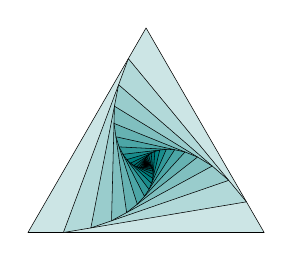
\begin{tikzpicture}[scale=.25]
  \tkzDefPoints{00/0/A,12/0/B,6/12*sind(60)/C}
  \foreach \density in {20,30,...,240}{%
    \tkzDrawPolygon[fill=teal!\density](A,B,C)
    \pgfnodealias{X}{A}
    \tkzDefPointWith[linear,K=.15](A,B) \tkzGetPoint{A}
    \tkzDefPointWith[linear,K=.15](B,C) \tkzGetPoint{B}
    \tkzDefPointWith[linear,K=.15](C,X) \tkzGetPoint{C}}
  \end{tikzpicture}
\end{tkzexample}

\vspace*{12pt}

\subsection{Why \tkzname{\tkznameofpack}? }
My initial goal was to provide other mathematics teachers and myself with a tool to quickly create Euclidean geometry figures without investing too much effort in learning a new programming language.
Of course, \tkzname{\tkznameofpack}  is for math teachers who use \LATEX\ and  makes it possible to easily create correct  drawings by means of \LATEX.

It appeared that the simplest method was to reproduce the one used to obtain construction by hand. 
To describe a construction, you must, of course, define the objects but also the actions that you perform. It seemed to me that syntax close to the language of mathematicians and their students would be more easily understandable; moreover, it also seemed to me that this syntax should be close to that of \LaTeX. 
The objects, of course, are points, segments, lines, triangles, polygons and circles. As for actions, I considered five to be sufficient, namely: define, create, draw, mark and label.

The syntax is perhaps too verbose but it is, I believe, easily accessible.
As a result, the students like teachers were able to easily access this tool.

\subsection{\tkzname{\tkznameofpack}  vs \tkzname{\TIKZ } }

I love programming with  \TIKZ,  and without  \TIKZ\  I would never have had the idea to create \tkzname{\tkznameofpack}  but never forget that behind it there is  \TIKZ\  and that it is always possible to insert code from  \TIKZ. \tkzname{\tkznameofpack}  doesn't prevent you from using  \TIKZ.
That said, I don't think mixing syntax is a good thing. 

There is no need to compare \TIKZ\  and \tkzname{\tkznameofpack}.  The latter is not addressed to the same audience as  \TIKZ. The first one allows you to do a lot of things, the second one only does geometry drawings. The first one can do everything the second one does, but the second one will more easily do what you want.

\subsection{How it works}

\subsubsection{Example Part I: gold triangle}
\begin{center}
\begin{tikzpicture}
  
\tkzDefPoint(0,0){C} % possible \tkzDefPoint[label=below:$C$](0,0){C} but don't do this
\tkzDefPoint(2,6){B}
% We get D and E with a rotation
\tkzDefPointBy[rotation= center B angle 36](C) \tkzGetPoint{D} 
\tkzDefPointBy[rotation= center B angle 72](C) \tkzGetPoint{E} 
% Toget A we use an intersection of lines
\tkzInterLL(B,E)(C,D) \tkzGetPoint{A}
\tkzInterLL(C,E)(B,D) \tkzGetPoint{H}
% drawing
\tkzDrawArc[delta=10](B,C)(E)
\tkzDrawPolygon(C,B,D)
\tkzDrawSegments(D,A B,A C,E)
% angles 
\tkzMarkAngles(C,B,D E,A,D) %this is to draw the arcs
\tkzLabelAngles[pos=1.5](C,B,D E,A,D){$\alpha$}
\tkzMarkRightAngle(B,H,C)
\tkzDrawPoints(A,...,E)
% Label only now
\tkzLabelPoints[below left](C,A)
\tkzLabelPoints[below right](D)
\tkzLabelPoints[above](B,E)
\end{tikzpicture}
\end{center}

Let's analyze the figure
\begin{enumerate}
  \item $CBD$ and $DBE$ are isosceles triangles; 
  
  \item $BC=BE$ and $(BD)$ is a bisector of the angle $CBE$;
  
  \item From this we deduce that the $CBD$ and $DBE$ angles are equal and have the same measure $\alpha$
   \[\widehat{BAC} +\widehat{ABC} + \widehat{BCA}=180^\circ \ \text{in the triangle}\ BAC \]
   \[3\alpha + \widehat{BCA}=180^\circ\  \text{in the triangle}\ CBD\]
   then 
     \[\alpha + 2\widehat{BCA}=180^\circ \] 
   or 
     \[\widehat{BCA}=90^\circ -\alpha/2 \] 
    
    \item  Finally   \[\widehat{CBD}=\alpha=36^\circ \] 
     the triangle $CBD$ is a "gold" triangle.
\end{enumerate}

\vspace*{24pt}
How construct a gold triangle or an angle of $36^\circ$?

\begin{enumerate}
  \item We place the fixed points $C$ and $D$. |\tkzDefPoint(0,0){C}| and |\tkzDefPoint(4,0){D}|;
  \item  We construct a square $CDef$ and we construct the midpoint $m$ of $[Cf]$;
  
  We can do all of this with a compass and a rule;
  \item Then we trace an arc with center $m$ through $e$. This arc cross the line $(Cf)$ at $n$;
  \item Now the two arcs with center $C$ and $D$ and radius $Cn$ define the point $B$.
\end{enumerate}


\begin{minipage}{.4\textwidth}
  \begin{tikzpicture}
  \tkzDefPoint(0,0){C}
  \tkzDefPoint(4,0){D}
  \tkzDefSquare(C,D)                     
  \tkzGetPoints{e}{f}
  \tkzDefMidPoint(C,f)                   
  \tkzGetPoint{m}
  \tkzInterLC(C,f)(m,e)                  
  \tkzGetSecondPoint{n}
  \tkzInterCC[with nodes](C,C,n)(D,C,n) 
  \tkzGetFirstPoint{B}
  \tkzDrawSegment[brown,dashed](f,n)
  \pgfinterruptboundingbox 
  \tkzDrawPolygon[brown,dashed](C,D,e,f)
  \tkzDrawArc[brown,dashed](m,e)(n)
  \tkzCompass[brown,dashed,delta=20](C,B)
  \tkzCompass[brown,dashed,delta=20](D,B)
  \endpgfinterruptboundingbox 
  \tkzDrawPoints(C,D,B)
  \tkzDrawPolygon(B,...,D)
  \end{tikzpicture}
\end{minipage}
\begin{minipage}{.6\textwidth}
  \begin{tkzexample}[code only,small]
  \begin{tikzpicture}
  \tkzDefPoint(0,0){C}
  \tkzDefPoint(4,0){D}
  \tkzDefSquare(C,D)                     
  \tkzGetPoints{e}{f}
  \tkzDefMidPoint(C,f)                   
  \tkzGetPoint{m}
  \tkzInterLC(C,f)(m,e)                  
  \tkzGetSecondPoint{n}
  \tkzInterCC[with nodes](C,C,n)(D,C,n) 
  \tkzGetFirstPoint{B}
  \tkzDrawSegment[brown,dashed](f,n)
  \pgfinterruptboundingbox 
  \tkzDrawPolygon[brown,dashed](C,D,e,f)
  \tkzDrawArc[brown,dashed](m,e)(n)
  \tkzCompass[brown,dashed,delta=20](C,B)
  \tkzCompass[brown,dashed,delta=20](D,B)
  \endpgfinterruptboundingbox 
  \tkzDrawPoints(C,D,B)
  \tkzDrawPolygon(B,...,D)
  \end{tikzpicture}
  \end{tkzexample}
\end{minipage}


After building the golden triangle $BCD$, we build the point $A$ by noticing that $BD=DA$. Then we get the point $E$ and finally the point $F$. This is done with already intersections of defined objects  (line and circle).
 

\begin{center}
  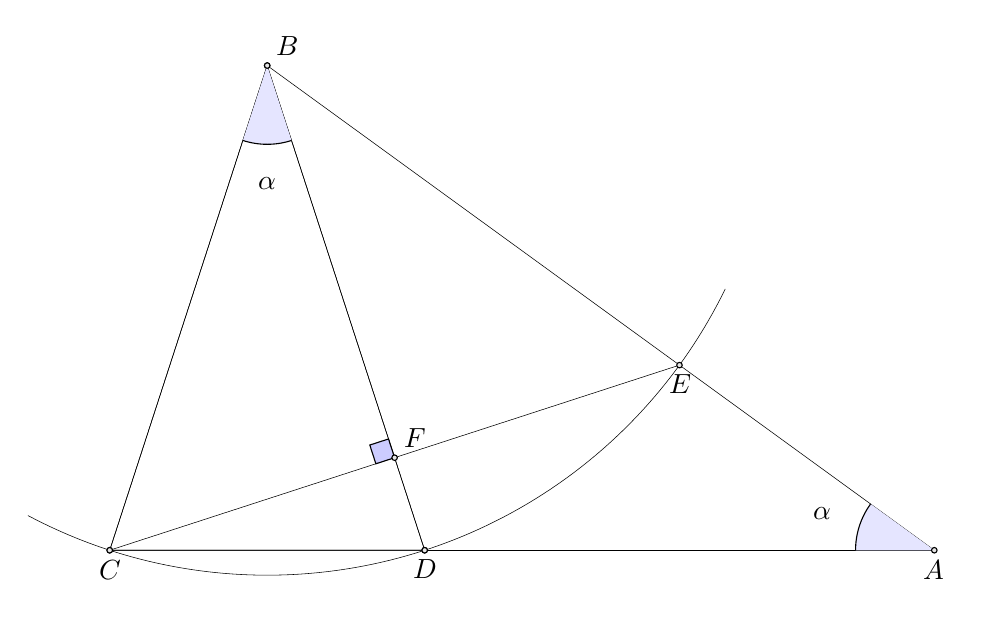
\begin{tikzpicture}
    \tkzDefPoint(0,0){C}
    \tkzDefPoint(4,0){D}
    \tkzDefSquare(C,D)                     
    \tkzGetPoints{e}{f}
    \tkzDefMidPoint(C,f)                   
    \tkzGetPoint{m}
    \tkzInterLC(C,f)(m,e)                  
    \tkzGetSecondPoint{n}
    \tkzInterCC[with nodes](C,C,n)(D,C,n) 
    \tkzGetFirstPoint{B}
    \tkzInterLC(C,D)(D,B) \tkzGetSecondPoint{A}
    \tkzInterLC(B,A)(B,D) \tkzGetSecondPoint{E}
    \tkzInterLL(B,D)(C,E) \tkzGetPoint{F}
    \tkzDrawPoints(C,D,B)
    \tkzDrawPolygon(B,...,D)  
    \tkzDrawPolygon(B,C,D)
    \tkzDrawSegments(D,A A,B C,E)
    \tkzDrawArc[delta=10](B,C)(E)
    \tkzMarkRightAngle[fill=blue!20](B,F,C)  
    \tkzFillAngles[fill=blue!10](C,B,D E,A,D)
    \tkzMarkAngles(C,B,D E,A,D)
    \tkzLabelAngles[pos=1.5](C,B,D E,A,D){$\alpha$} 
    \tkzLabelPoints[below](A,C,D,E)
    \tkzLabelPoints[above right](B,F)
    \tkzDrawPoints(A,...,F) 
  \end{tikzpicture} 
\end{center}



\begin{tkzexample}[code only,small]
  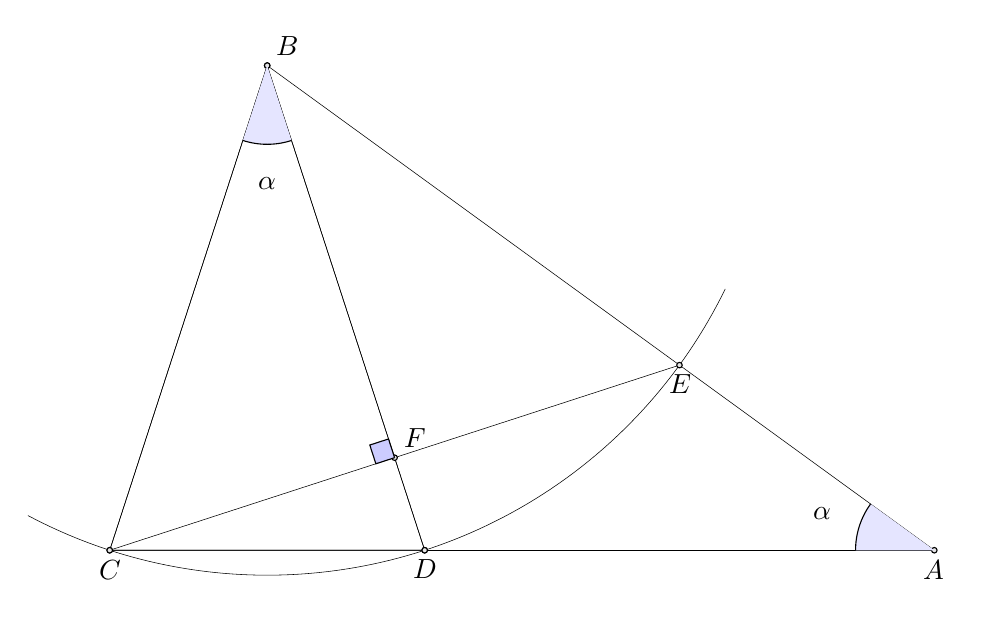
\begin{tikzpicture}
    \tkzDefPoint(0,0){C}
    \tkzDefPoint(4,0){D}
    \tkzDefSquare(C,D)                     
    \tkzGetPoints{e}{f}
    \tkzDefMidPoint(C,f)                   
    \tkzGetPoint{m}
    \tkzInterLC(C,f)(m,e)                  
    \tkzGetSecondPoint{n}
    \tkzInterCC[with nodes](C,C,n)(D,C,n) 
    \tkzGetFirstPoint{B}
    \tkzInterLC(C,D)(D,B) \tkzGetSecondPoint{A}
    \tkzInterLC(B,A)(B,D) \tkzGetSecondPoint{E}
    \tkzInterLL(B,D)(C,E) \tkzGetPoint{F}
    \tkzDrawPoints(C,D,B)
    \tkzDrawPolygon(B,...,D)  
    \tkzDrawPolygon(B,C,D)
    \tkzDrawSegments(D,A A,B C,E)
    \tkzDrawArc[delta=10](B,C)(E)
    \tkzDrawPoints(A,...,F) 
    \tkzMarkRightAngle[fill=blue!20](B,F,C)  
    \tkzFillAngles[fill=blue!10](C,B,D E,A,D)
    \tkzMarkAngles(C,B,D E,A,D)
    \tkzLabelAngles[pos=1.5](C,B,D E,A,D){$\alpha$} 
    \tkzLabelPoints[below](A,C,D,E)
    \tkzLabelPoints[above right](B,F)
  \end{tikzpicture} 
\end{tkzexample}

\subsubsection{Example Part II: two others methods gold and euclide triangle}

\tkzname{\tkznameofpack} knows how to define a "gold" or "euclide" triangle. We can define $BCD$ and $BCA$ like gold triangles.


  \begin{center}
    \begin{tkzexample}[code only,small]
      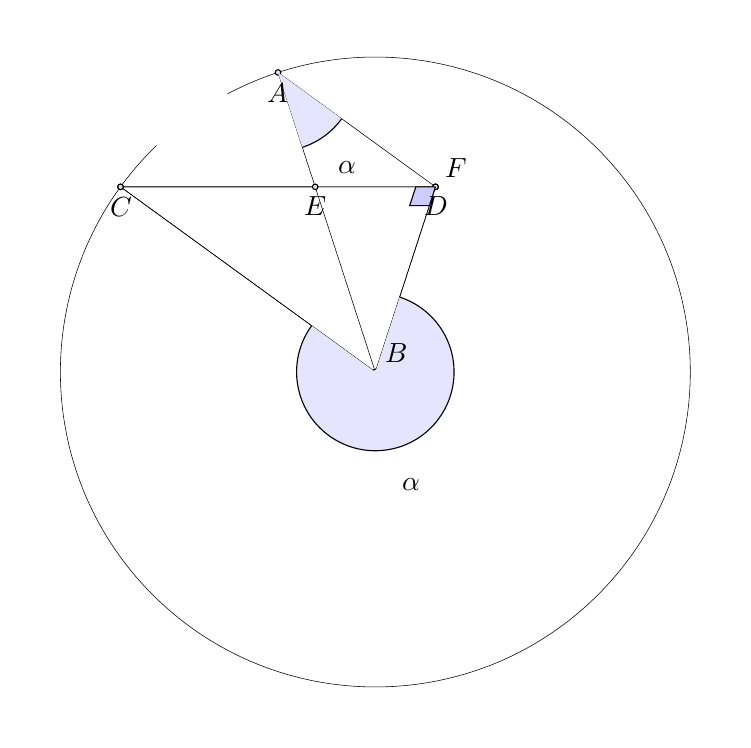
\begin{tikzpicture}
        \tkzDefPoint(0,0){C}
        \tkzDefPoint(4,0){D}
        \tkzDefTriangle[euclide](C,D)
        \tkzGetPoint{B}
        \tkzDefTriangle[euclide](B,C)
        \tkzGetPoint{A}
        \tkzInterLC(B,A)(B,D) \tkzGetSecondPoint{E}
        \tkzInterLL(B,D)(C,E) \tkzGetPoint{F}
        \tkzDrawPoints(C,D,B)
        \tkzDrawPolygon(B,...,D)  
        \tkzDrawPolygon(B,C,D)
        \tkzDrawSegments(D,A A,B C,E)
        \tkzDrawArc[delta=10](B,C)(E)
        \tkzDrawPoints(A,...,F) 
        \tkzMarkRightAngle[fill=blue!20](B,F,C)  
        \tkzFillAngles[fill=blue!10](C,B,D E,A,D)
        \tkzMarkAngles(C,B,D E,A,D)
        \tkzLabelAngles[pos=1.5](C,B,D E,A,D){$\alpha$} 
        \tkzLabelPoints[below](A,C,D,E)
        \tkzLabelPoints[above right](B,F)
      \end{tikzpicture} 
    \end{tkzexample}
  \end{center}

Here is a final method that uses rotations:  

\begin{center}
  \begin{tkzexample}[code only,small]
  \begin{tikzpicture} 
  \tkzDefPoint(0,0){C} % possible 
  % \tkzDefPoint[label=below:$C$](0,0){C} 
  % but don't do this
  \tkzDefPoint(2,6){B}
  % We get D and E with a rotation
  \tkzDefPointBy[rotation= center B angle 36](C) \tkzGetPoint{D} 
  \tkzDefPointBy[rotation= center B angle 72](C) \tkzGetPoint{E} 
  % To get A we use an intersection of lines
  \tkzInterLL(B,E)(C,D) \tkzGetPoint{A}
  \tkzInterLL(C,E)(B,D) \tkzGetPoint{H}
  % drawing
  \tkzDrawArc[delta=10](B,C)(E)
  \tkzDrawPolygon(C,B,D)
  \tkzDrawSegments(D,A B,A C,E)
  % angles 
  \tkzMarkAngles(C,B,D E,A,D) %this is to draw the arcs
  \tkzLabelAngles[pos=1.5](C,B,D E,A,D){$\alpha$}
  \tkzMarkRightAngle(B,H,C)
  \tkzDrawPoints(A,...,E)
  % Label only now
  \tkzLabelPoints[below left](C,A)
  \tkzLabelPoints[below right](D)
  \tkzLabelPoints[above](B,E)
  \end{tikzpicture}
  \end{tkzexample}
\end{center}


\subsubsection{Complete but minimal example}


A unit of length being chosen, the example shows how to obtain a segment of length $\sqrt{a}$ from a segment of length $a$, using a ruler and a compass.

$IB=a$, $AI=1$

\vspace{12pt}
\hypertarget{firstex}{}

\begin{tikzpicture}[scale=1,ra/.style={fill=gray!20}]
   % fixed points
   \tkzDefPoint(0,0){A}
   \tkzDefPoint(1,0){I}
   % calculation
   \tkzDefPointBy[homothety=center A ratio  10 ](I) \tkzGetPoint{B}  
   \tkzDefMidPoint(A,B)              \tkzGetPoint{M}
   \tkzDefPointWith[orthogonal](I,M) \tkzGetPoint{H}
   \tkzInterLC(I,H)(M,B)             \tkzGetSecondPoint{C}
   \tkzDrawSegment[style=orange](I,C)
   \tkzDrawArc(M,B)(A)
   \tkzDrawSegment[dim={$1$,-16pt,}](A,I)
   \tkzDrawSegment[dim={$a/2$,-10pt,}](I,M)
   \tkzDrawSegment[dim={$a/2$,-16pt,}](M,B)   
   \tkzMarkRightAngle[ra](A,I,C)
   \tkzDrawPoints(I,A,B,C,M)  
   \tkzLabelPoint[left](A){$A(0,0)$} 
   \tkzLabelPoints[above right](I,M)
   \tkzLabelPoints[above left](C)
   \tkzLabelPoint[right](B){$B(10,0)$}
   \tkzLabelSegment[right=4pt](I,C){$\sqrt{a^2}=a \ (a>0)$}
\end{tikzpicture}

\emph{Comments}
 
\begin{itemize}
\item The Preamble


 Let us first look at the preamble. If you need it, you have to load \tkzname{xcolor} before \tkzname{tkz-euclide}, that is, before \TIKZ. \TIKZ\ may cause problems with the active characters, but...
 provides a library in its latest version that's supposed to solve these problems \NameLib{babel}.
 
\begin{tkzltxexample}[]
\documentclass{standalone} % or another class
   % \usepackage{xcolor} % before tikz or tkz-euclide if necessary
\usepackage{tkz-euclide} % no need to load TikZ
   % \usetkzobj{all}  is no longer necessary 
   % \usetikzlibrary{babel}  if there are problems with the active characters
\end{tkzltxexample}

The following code consists of several parts:

   \item  Definition of fixed points: the first part includes the definitions of the points necessary for the construction, these are the fixed points. The macros \tkzcname{tkzInit} and \tkzcname{tkzClip} in most cases are not necessary.

\begin{tkzltxexample}[]
  \tkzDefPoint(0,0){A}
  \tkzDefPoint(1,0){I}
\end{tkzltxexample}
 
  \item The second part is dedicated to the creation of new points from the fixed points;
  a $B$ point is placed at $10$~cm    from $A$. The middle of $[AB]$ is defined by $M$ and then the orthogonal line to the $(AB)$ line is searched for at the $I$ point. Then we look for the intersection of this line with the semi-circle of center $M$ passing through $A$.  
  
\begin{tkzltxexample}[]
   \tkzDefPointBy[homothety=center A ratio  10 ](I)
      \tkzGetPoint{B}
   \tkzDefMidPoint(A,B)
      \tkzGetPoint{M}
   \tkzDefPointWith[orthogonal](I,M)
      \tkzGetPoint{H}
   \tkzInterLC(I,H)(M,A)
      \tkzGetSecondPoint{B}
 \end{tkzltxexample}  
     

 \item The third one includes the different drawings;
 \begin{tkzltxexample}[]
   \tkzDrawSegment[style=orange](I,H)
   \tkzDrawPoints(O,I,A,B,M)
   \tkzDrawArc(M,A)(O)
   \tkzDrawSegment[dim={$1$,-16pt,}](O,I)  
   \tkzDrawSegment[dim={$a/2$,-10pt,}](I,M)
   \tkzDrawSegment[dim={$a/2$,-16pt,}](M,A)
 \end{tkzltxexample}
 
\item  Marking: the fourth is devoted to marking;


\begin{tkzltxexample}[]
   \tkzMarkRightAngle(A,I,B)
 \end{tkzltxexample}
 
 \item Labelling: the latter only deals with the placement of labels.
\begin{tkzltxexample}[]
   \tkzLabelPoint[left](O){$A(0,0)$}
   \tkzLabelPoint[right](A){$B(10,0)$}
   \tkzLabelSegment[right=4pt](I,B){$\sqrt{a^2}=a \ (a>0)$}
\end{tkzltxexample}


\item The full code:


\begin{tkzexample}[code only]
  \begin{tikzpicture}[scale=1,ra/.style={fill=gray!20}]
     % fixed points
     \tkzDefPoint(0,0){A}
     \tkzDefPoint(1,0){I}
     % calculation
     \tkzDefPointBy[homothety=center A ratio  10 ](I) \tkzGetPoint{B}  
     \tkzDefMidPoint(A,B)              \tkzGetPoint{M}
     \tkzDefPointWith[orthogonal](I,M) \tkzGetPoint{H}
     \tkzInterLC(I,H)(M,B)             \tkzGetSecondPoint{C}
     \tkzDrawSegment[style=orange](I,C)
     \tkzDrawArc(M,B)(A)
     \tkzDrawSegment[dim={$1$,-16pt,}](A,I)
     \tkzDrawSegment[dim={$a/2$,-10pt,}](I,M)
     \tkzDrawSegment[dim={$a/2$,-16pt,}](M,B)   
     \tkzMarkRightAngle[ra](A,I,C)
     \tkzDrawPoints(I,A,B,C,M)  
     \tkzLabelPoint[left](A){$A(0,0)$} 
     \tkzLabelPoints[above right](I,M)
     \tkzLabelPoints[above left](C)
     \tkzLabelPoint[right](B){$B(10,0)$}
     \tkzLabelSegment[right=4pt](I,C){$\sqrt{a^2}=a \ (a>0)$}
  \end{tikzpicture}
\end{tkzexample}
\end{itemize}

\subsection{The Elements of tkz code}
In this paragraph, we start looking at the "rules" and "symbols" used to create a figure with \tkzname{\tkznameofpack}.

 The primitive objects are points. You can refer to a point at any time using the name given when defining it. (it is possible to assign a different name later on).

\medskip
In general, \tkzname{\tkznameofpack} macros have a name beginning with tkz. There are four main categories starting with:
|\tkzDef...| |\tkzDraw...| |\tkzMark...| and |\tkzLabel...|

Among the first category, |\tkzDefPoint| allows you to define fixed points. It will be studied in detail later. Here we will see in detail the macro  |\tkzDefTriangle|.

This macro makes it possible to associate to a pair of points a third point in order to define a certain triangle |\tkzDefTriangle(A,B)|. The obtained point is referenced |tkzPointResult| and it is possible to choose another reference with |\tkzGetPoint{C}| for example.
Parentheses are used to pass arguments. In |(A,B)| $A$ and $B$ are the points with which a third will be defined.

However, in |{C}| we use braces to retrieve the new point.
In order to choose a certain type of triangle among the following choices:
  |equilateral|, |half|, |pythagoras|, |school|, |golden or sublime|, |euclide|, |gold|, |cheops|...
 and |two angles| you just have to choose between hooks, for example:
 
|\tkzDefTriangle[euclide](A,B) \tkzGetPoint{C}|

\begin{minipage}{0.5\textwidth}
  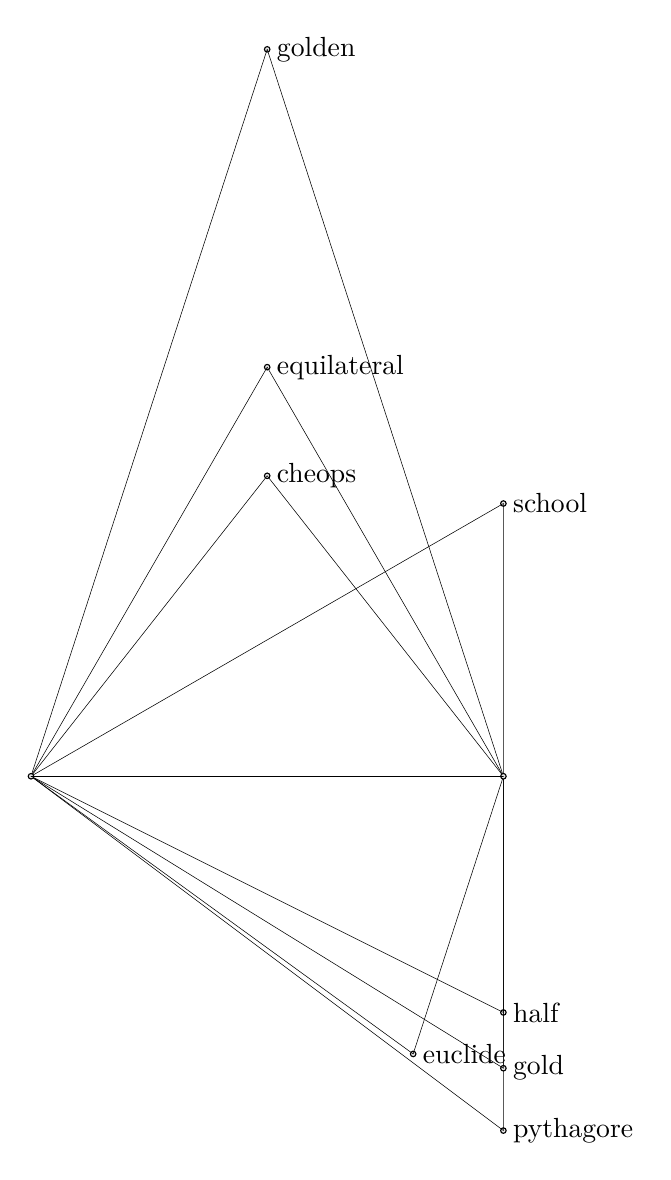
\begin{tikzpicture}[scale=.75]
  \tkzDefPoints{0/0/A,8/0/B}
  \foreach \tr in {equilateral,half,pythagore,%
          school,golden,euclide, gold,cheops}
  {\tkzDefTriangle[\tr](A,B) \tkzGetPoint{C}
  \tkzDrawPoint(C)
  \tkzLabelPoint[right](C){\tr}
  \tkzDrawSegments(A,C C,B)}
  \tkzDrawPoints(A,B)
  \tkzDrawSegments(A,B)
  \end{tikzpicture}
\end{minipage}
\begin{minipage}{0.5\textwidth}
  \begin{tkzexample}[code only,small]
    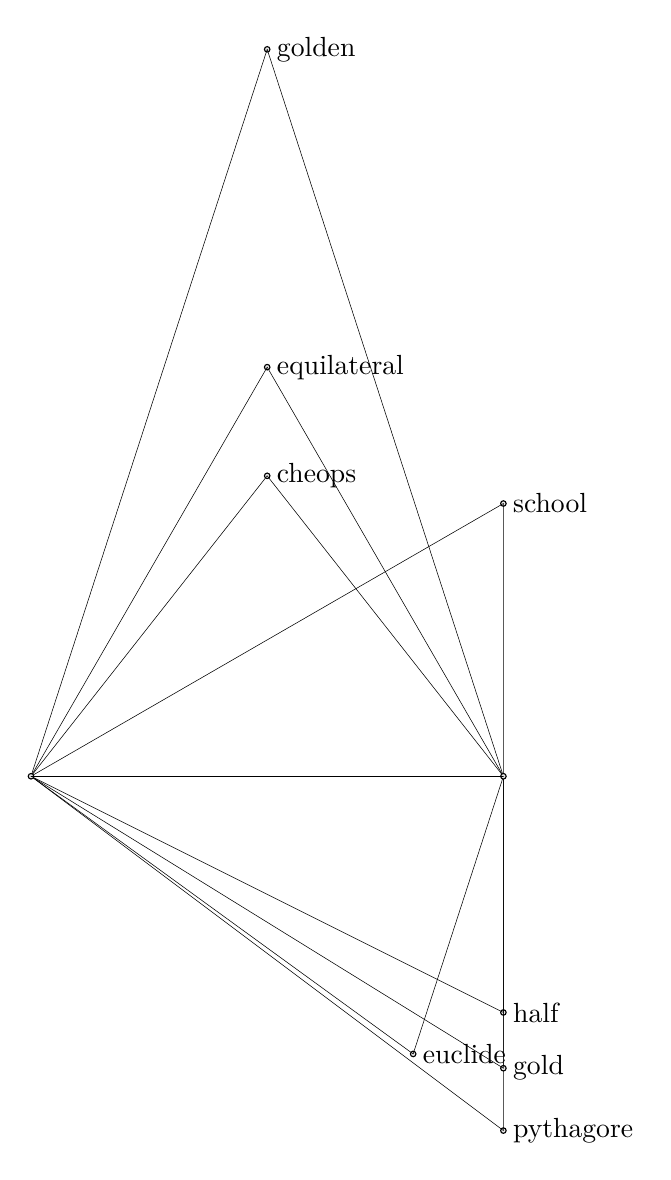
\begin{tikzpicture}[scale=.75]
    \tkzDefPoints{0/0/A,8/0/B}
    \foreach \tr in {equilateral,half,pythagore,%
            school,golden,euclide, gold,cheops}
    {\tkzDefTriangle[\tr](A,B) \tkzGetPoint{C}
    \tkzDrawPoint(C)
    \tkzLabelPoint[right](C){\tr}
    \tkzDrawSegments(A,C C,B)}
    \tkzDrawPoints(A,B)
    \tkzDrawSegments(A,B)
    \end{tikzpicture}
  \end{tkzexample}

\end{minipage}


\subsection{Notations and conventions}

I deliberately chose to use the geometric French and personal  conventions  to describe the geometric objects represented. The objects defined and represented by \tkzname{\tkznameofpack} are points, lines and circles located in a plane. They are the primary objects of Euclidean geometry from which we will construct figures.

According to \tkzimp{Euclidian} these figures will only illustrate pure ideas produced by our brain.
Thus a point has no dimension and therefore no real existence. In the same way the line has no width and therefore no existence in the real world. The objects that we are going to consider are only representations of ideal mathematical objects. \tkzname{\tkznameofpack} will follow the steps of the ancient Greeks to obtain geometrical constructions using the ruler and the compass. 

Here are the notations that will be used:


\begin{itemize}
\item The points are represented geometrically either by a small disc or by the intersection of two lines (two straight lines, a straight line and a circle or two circles). In this case, the point is represented by a cross. 

\begin{tkzexample}[latex=6cm, small]     
  \begin{tikzpicture}       
    \tkzDefPoints{0/0/A,4/2/B}       
    \tkzDrawPoints(A,B)       
    \tkzLabelPoints(A,B)     
  \end{tikzpicture}    
\end{tkzexample}

or else

\begin{tkzexample}[latex=6cm, small]     
  \begin{tikzpicture}       
    \tkzSetUpPoint[shape=cross, color=red]       
    \tkzDefPoints{0/0/A,4/2/B}       
    \tkzDrawPoints(A,B)       
    \tkzLabelPoints(A,B)     
    \end{tikzpicture}    
    \end{tkzexample}  

The existence of a point being established, we can give it a label which will be a capital letter (with some exceptions) of the Latin alphabet such as $A$, $B$ or $C$. For example:
\begin{itemize}
\item $O$ is a center for a circle, a rotation, etc.;
\item $M$ defined a midpoint;
\item $H$ defined the foot of an altitude;
\item $P'$ is the image of $P$ by a transformation ;
\end{itemize}

It is important to note that the reference name of a point in the code may be different from the label to designate it in the text. So we can define a point A and give it as label $P$. In particular the style will be different, point A will be labeled $A$. 

\begin{tkzexample}[latex=6cm, small]     
  \begin{tikzpicture}       
    \tkzDefPoints{0/0/A}       
    \tkzDrawPoints(A)       
    \tkzLabelPoint(A){$P$}     
  \end{tikzpicture}    
\end{tkzexample}

Exceptions: some points such as the middle of the sides of a triangle share a characteristic, so it is normal that their names also share a common character. We will designate these points by $M_a$, $M_b$ and $M_c$ or $M_A$, $M_B$ and $M_C$.

In the code, these points will be referred to as: M\_A, M\_B and M\_C.

Another exception relates to intermediate construction points which will not be labelled. They will often be designated by a lowercase letter in the code.

\item The line segments are designated by two points representing their ends in square brackets: $[AB]$. 

\item The straight lines are in Euclidean geometry defined by two points so $A$ and $B$ define the straight line $(AB)$. We can also designate this stright line using the Greek alphabet and name it $(\delta)$ or $(\Delta)$. It is also possible to designate the straight line with lowercase letters such as $d$ and $d'$.

\item The semi-straight line is designated as follows $[AB)$.


\item Relation between the straight lines. Two perpendicular $(AB)$ and $(CD)$ lines will be written $(AB) \perp (CD)$ and if they are parallel we will write $(AB) \parallelslant (CD)$.

\item The lengths of the sides of triangle ABC are $AB$, $AC$ and $BC$. The numbers are also designated by a lowercase letter so we will write: $AB=c$, $AC=b$ and $BC=a$. The letter $a$ is also used to represent an angle, and $r$ is frequently used to represent a radius, $d$ a diameter, $l$ a length, $d$ a distance.

\item Polygons are designated afterwards by their vertices so $ABC$ is a triangle, $EFGH$ a quadrilateral.

\item Angles are generally measured in degrees (ex $60^\circ$) and in an equilateral $ABC$ triangle we will write $\widehat{ABC}=\widehat{B}=60^\circ$.

\item The arcs are designated by their extremities. For example if $A$ and $B$ are two points of the same circle then $\widearc{AB}$.


\item Circles are noted either $\mathcal{C}$ if there is no possible confusion or $\mathcal{C}$ $(O~;~A)$ for a circle with center $O$ and passing through the point $A$ or $\mathcal{C}$ $(O~;~1)$ for a circle with center O and radius 1 cm.

\item  Name of the particular lines of a triangle: I used the terms bisector, bisector out, mediator (sometimes called perpendicular bisectors), altitude, median and symmedian.

\item ($x_1$,$y_1$) coordinates of the point $A_1$, ($x_A$,$y_A$) coordinates of the point $A$.

\end{itemize}




\subsection{How to use the \tkzname{\tkznameofpack} package ?}
\subsubsection{Let's look at a classic example}
In order to show the right way, we will see how to build an equilateral triangle. Several possibilities are open to us, we are going to follow the steps of Euclid.

\begin{itemize}
\item   First of all you have to use a document class. The best choice to test your code is to create a single figure with the class \tkzname{standalone}\index{standalone}.
\begin{verbatim}  
\documentclass{standalone}
\end{verbatim}
\item Then load the \tkzname{\tkznameofpack} package:
\begin{verbatim}  
\usepackage{tkz-euclide}
\end{verbatim}

 You don't need to load \TIKZ\ because the \tkzname{\tkznameofpack} package works on top of TikZ and loads it.
 \item  {\color{red} \bomb \sout{|\BS usetkzobj{all}| }}
 With the new version 3.03 you don't need this line anymore. All objects are now loaded.
 \item Start the document and open a TikZ picture environment:
\begin{verbatim}
\begin{document}
\begin{tikzpicture}
\end{verbatim}

\item Now we define two fixed points:
\begin{verbatim}
\tkzDefPoint(O,O){A}
\tkzDefPoint(5,2){B}
\end{verbatim}

\item Two points define two circles, let's use these circles:

 circle with center $A$ through $B$ and circle with center $B$ through $A$. These two circles have two points in common.
\begin{verbatim}
\tkzInterCC(A,B)(B,A)
\end{verbatim}
We can get the points of intersection with
\begin{verbatim}
\tkzGetPoints{C}{D}
\end{verbatim}

\item All the necessary points are obtained, we can move on to the final steps including the plots.
\begin{verbatim}
\tkzDrawCircles[gray,dashed](A,B B,A)
\tkzDrawPolygon(A,B,C)% The triangle
\end{verbatim}
\item Draw all points $A$, $B$, $C$ and $D$:
\begin{verbatim}
\tkzDrawPoints(A,...,D)
\end{verbatim}

\item The final step, we print labels to the points and use options for positioning:\\
\begin{verbatim}
\tkzLabelSegments[swap](A,B){$c$}
\tkzLabelPoints(A,B,D)
\tkzLabelPoints[above](C)
\end{verbatim}
\item We finally close both environments
\begin{verbatim}
\end{tikzpicture}
\end{document}
\end{verbatim}

\item The complete code

\begin{tkzexample}[latex=8cm,small]
 \begin{tikzpicture}[scale=.5]
   % fixed points
  \tkzDefPoint(0,0){A}
  \tkzDefPoint(5,2){B}
  % calculus
  \tkzInterCC(A,B)(B,A)
  \tkzGetPoints{C}{D}
  % drawings
  \tkzDrawCircles[gray,dashed](A,B B,A)
  \tkzDrawPolygon(A,B,C)
  \tkzDrawPoints(A,...,D)
  % marking
  \tkzMarkSegments[mark=s||](A,B B,C C,A)
  % labelling
  \tkzLabelSegments[swap](A,B){$c$}
  \tkzLabelPoints(A,B,D)
  \tkzLabelPoints[above](C)
\end{tikzpicture}
\end{tkzexample}

 \end{itemize}

\subsubsection{\tkzname{Set, Calculate, Draw, Mark, Label}}
The title could have been: \texttt{Separation of Calculus and Drawings}

When a document is prepared using the \LATEX\ system, the source code of the document can be divided into two parts: the document body and the preamble.
Under this methodology,  publications can be structured, styled and typeset with minimal effort.
I propose a similar methodology for creating figures with \tkzname{\tkznameofpack}.

The first part defines the fixed points, the second part allows the creation of new points. These are the two main parts. All that is left to do is to draw, mark and label.




\endinput














 \section{Installation}

\tkzNamePack{tkz-euclide} and \tkzNamePack{tkz-base} are now on the server of the \tkzname{CTAN}\footnote{\tkzNamePack{tkz-base} and \tkzNamePack{tkz-euclide} are part of \NameDist{TeXLive} and \tkzname{tlmgr} allows you to install them. These packages are also part of \NameDist{MiKTeX} under \NameSys{Windows}.}. If you want to test a beta version, just put the following files in a texmf folder that your system can find.
You will have to check several points:

\begin{itemize}\setlength{\itemsep}{5pt}
\item  The \tkzNamePack{tkz-base} and \tkzNamePack{tkz-euclide} folders must be located on a path recognized by \tkzname{latex}.
\item  The \tkzNamePack{xfp}\footnote{\tkzNamePack{xfp} replaces \tkzNamePack{fp}.}, \tkzNamePack{numprint} and \tkzNamePack{tikz 3.00} must be installed as they are mandatory, for the proper functioning of \tkzNamePack{tkz-euclide}.
\item This documentation and all examples were obtained with \tkzname{lualatex-dev} but \tkzname{pdflatex} should be suitable.
\end{itemize}

\subsection{List of folder files \tkzname{tkzbase}  and \tkzname{tkzeuclide}}

In the folder \tkzname{base}:

\begin{itemize}
\item  \tkzname{tkz-base.cfg}
\item  \tkzname{tkz-base.sty}
\item  \tkzname{tkz-lib-marks.tex}
\item  \tkzname{tkz-obj-axes.tex}
\item  \tkzname{tkz-obj-grids.tex}
\item  \tkzname{tkz-obj-marks.tex}
\item  \tkzname{tkz-obj-points.tex}
\item  \tkzname{tkz-obj-rep.tex}
\item  \tkzname{tkz-tools-arith.tex}
\item  \tkzname{tkz-tools-base.tex}
\item  \tkzname{tkz-tools-BB.tex}
\item  \tkzname{tkz-tools-misc.tex}
\item  \tkzname{tkz-tools-modules.tex}
\item  \tkzname{tkz-tools-print.tex}
\item  \tkzname{tkz-tools-text.tex}
\item  \tkzname{tkz-tools-utilities.tex}
\end{itemize}

In the folder \tkzname{euclide}:

\begin{itemize}
\item   \tkzname{tkz-euclide.sty}
\item   \tkzname{tkz-obj-eu-angles.tex}
\item   \tkzname{tkz-obj-eu-arcs.tex}
\item   \tkzname{tkz-obj-eu-circles.tex}
\item   \tkzname{tkz-obj-eu-compass.tex}
\item   \tkzname{tkz-obj-eu-draw-circles.tex}
\item   \tkzname{tkz-obj-eu-draw-lines.tex}
\item   \tkzname{tkz-obj-eu-draw-polygons.tex}
\item   \tkzname{tkz-obj-eu-draw-triangles.tex}
\item   \tkzname{tkz-obj-eu-lines.tex}
\item   \tkzname{tkz-obj-eu-points-by.tex}
\item   \tkzname{tkz-obj-eu-points-rnd.tex}
\item   \tkzname{tkz-obj-eu-points-with.tex}
\item   \tkzname{tkz-obj-eu-points.tex}
\item   \tkzname{tkz-obj-eu-polygons.tex}
\item   \tkzname{tkz-obj-eu-protractor.tex}
\item   \tkzname{tkz-obj-eu-sectors.tex}
\item   \tkzname{tkz-obj-eu-show.tex}
\item   \tkzname{tkz-obj-eu-triangles.tex}
\item   \tkzname{tkz-tools-angles.tex}
\item   \tkzname{tkz-tools-intersections.tex}
\item   \tkzname{tkz-tools-math.tex}
\end{itemize}
\tkzHandBomb\ Now \tkzname{tkz-euclide} loads all the files.
\endinput

\section{News and compatibility}


Some changes have been made to make the syntax more homogeneous and especially to distinguish the definition and search for coordinates from the rest, i.e. drawing, marking and labelling.
In the future, the definition macros being isolated, it will be easier to introduce a phase of coordinate calculations using \tkzimp{Lua}.

An important novelty is the recent replacement of the \tkzNamePack{fp} package by \tkzNamePack{xfp}.  This is to improve the calculations a little bit more and to make it easier to use.


Here are some of the changes. 
\vspace{1cm}
 \begin{itemize}\setlength{\itemsep}{10pt} 

\item Improved code and bug fixes;

\item With \tkzimp{tkz-euclide} loads all objects, so there's no need to place \tkzcname{usetkzobj\{all\}};\item The bounding box is now controlled in each macro (hopefully) to avoid the use of \tkzcname{tkzInit} followed by \tkzcname{tkzClip};\item Added macros for the bounding box: \tkzcname{tkzSaveBB} \tkzcname{tkzClipBB} and so on;\item  Logically most macros accept \TIKZ\ options. So I removed the "duplicate" options when possible thus the "label options" option is removed;

\item Random points are now in \tkzname{\tkznameofpack} and the macro \tkzcname{tkzGetRandPointOn} is replaced by \tkzcname{tkzDefRandPointOn}. For homogeneity reasons, the points must be retrieved with \tkzcname{tkzGetPoint};

\item The options \tkzname{end} and \tkzname{start} which allowed to give a label to a straight  line are removed. You now have to use the macro \tkzcname{tkzLabelLine};

\item Introduction of the libraries \NameLib{quotes} and \NameLib{angles}; it allows to give a label to a point, even if I am not in favour of this practice;

\item  The notion of vector disappears, to draw a vector just pass "->" as an option to \tkzcname{tkzDrawSegment};

\item Many macros still exist, but are obsolete and will disappear:
\begin{itemize}

\item |\tkzDrawMedians| trace and create midpoints on the sides of a triangle. The creation and drawing separation is not respected so it is preferable to first create the coordinates of these points with |\tkzSpcTriangle[median]| and then to choose the ones you are going to draw with |\tkzDrawSegments| or |\tkzDrawLines|;

\item |\tkzDrawMedians(A,B)(C)| is now spelled |\tkzDrawMedians(A,C,B)|. This defines the median from $C$;
  
\item Another example |\tkzDrawTriangle[equilateral]| was handy but it is better to get the third point with |\tkzDefTriangle[equilateral]| and then draw with |\tkzDrawPolygon|;
  
\item |\tkzDefRandPointOn| is replaced by |\tkzGetRandPointOn|;\item now |\tkzTangent| is replaced by |\tkzDefTangent|;

\item You can use |global path name| if you want find intersection  but it's very slow like in \TIKZ.

\end{itemize}


\item Appearance of the macro \tkzcname{usetkztool} which allows to load new "tools".
\end{itemize}

\endinput
\section{Definition of a point}

 Points can be specified in any of the following ways:
\begin{itemize}
\item Cartesian coordinates;
\item Polar coordinates;
\item Named points;
\item Relative points.
\end{itemize}

Even if it's possible, I think it's a bad idea to work directly with coordinates. Preferable is to use named points.
A point is defined if it has a name linked to a unique pair of decimal numbers.
 Let $(x,y)$ or $(a:d)$  i.e. ($x$ abscissa, $y$ ordinate) or  ($a$ angle: $d$ distance).
 This is possible because the plan has been provided with an orthonormed Cartesian coordinate system.   The working axes are supposed to be (ortho)normed with unity equal to $1$~cm or something equivalent like $0.39370$~in.
 Now by default if you use a grid or axes, the rectangle used is defined by the coordinate points: $(0,0)$ and $(10,10)$. It's the macro \tkzcname{tkzInit} of the package \tkzNamePack{tkz-base} that creates this rectangle. Look at the following two codes and the result of their compilation:

\begin{tkzexample}[latex=10cm,small]

\begin{tikzpicture}
\tkzGrid
\tkzDefPoint(0,0){O}
\tkzDrawPoint[red](O)
\tkzShowBB[line width=2pt,teal]
\end{tikzpicture}
\end{tkzexample}


\begin{tkzexample}[latex=7cm,small]

\begin{tikzpicture}
 \tkzDefPoint(0,0){O}
 \tkzDefPoint(5,5){A}
 \tkzDrawSegment[blue](O,A)
 \tkzDrawPoints[red](O,A)
 \tkzShowBB[line width=2pt,teal]
\end{tikzpicture}
\end{tkzexample}

 The Cartesian coordinate $(a,b)$ refers to the
 point $a$ centimeters in the $x$-direction and $b$ centimeters in the
 $y$-direction.

 A point in polar coordinates requires an angle $\alpha$, in degrees,
 and a distance  $d$ from the origin with a dimensional
 unit by default it's the \texttt{cm}.


\begin{minipage}[b]{0.5\textwidth}
 Cartesian coordinates
\begin{tkzexample}[vbox,small]
\begin{tikzpicture}[scale=1]
  \tkzInit[xmax=5,ymax=5]
  \tkzDefPoints{0/0/O,1/0/I,0/1/J}
  \tkzDrawXY[noticks,>=latex]
  \tkzDefPoint(3,4){A}
  \tkzDrawPoints(O,A)
  \tkzLabelPoint(A){$A_1 (x_1,y_1)$}
  \tkzShowPointCoord[xlabel=$x_1$,
                     ylabel=$y_1$](A)
  \tkzLabelPoints(O,I)
  \tkzLabelPoints[left](J)
  \tkzDrawPoints[shape=cross](I,J)
\end{tikzpicture}
\end{tkzexample}%
\end{minipage}
\begin{minipage}[b]{0.5\textwidth}
 Polar coordinates
\begin{tkzexample}[vbox,small]
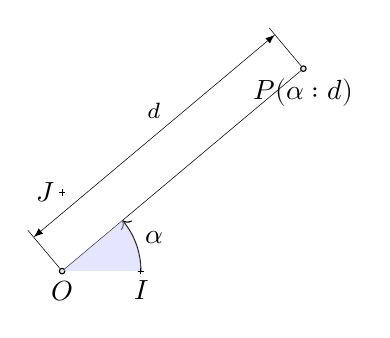
\begin{tikzpicture}[,scale=1]
  \tkzInit[xmax=5,ymax=5]
  \tkzDefPoints{0/0/O,1/0/I,0/1/J}
  \tkzDefPoint(40:4){P}
  \tkzDrawXY[noticks,>=triangle 45]
  \tkzDrawSegment[dim={$d$,
                 16pt,above=6pt}](O,P)
  \tkzDrawPoints(O,P)
  \tkzMarkAngle[mark=none,->](I,O,P)
  \tkzFillAngle[fill=blue!20,
                opacity=.5](I,O,P)
  \tkzLabelAngle[pos=1.25](I,O,P){$\alpha$}
  \tkzLabelPoint(P){$P  (\alpha : d )$}
  \tkzDrawPoints[shape=cross](I,J)
  \tkzLabelPoints(O,I)
  \tkzLabelPoints[left](J)
\end{tikzpicture}
\end{tkzexample}
\end{minipage}%

The \tkzNameMacro{tkzDefPoint} macro is used to define a point by assigning coordinates to it. This macro is based on \tkzNameMacro{coordinate}, a macro of \TIKZ. It can use \TIKZ-specific options such as \tkzname{shift}. If calculations are required then the \tkzNamePack{xfp} package is chosen. We can use Cartesian or polar coordinates.

\subsection{Defining a named point  \tkzcname{tkzDefPoint}}

\begin{NewMacroBox}{tkzDefPoint}{\oarg{local options}\parg{$x,y$}\marg{name} or \parg{$\alpha$:$d$}\marg{name}}%
\begin{tabular}{lll}%
arguments &  default & definition  \\
\midrule
\TAline{($x,y$)}{no default}{$x$ and $y$ are two dimensions, by default in cm.}
\TAline{($\alpha$:$d$)}{no default}{$\alpha$ is an angle in degrees, $d$ is a dimension}
\TAline{\{name\}}{no default}{Name assigned to the point: $A$, $T_a$ ,$P1$ etc ...}
\bottomrule
\end{tabular}

\medskip
The obligatory arguments of this macro are two dimensions expressed with decimals, in the first case they are two measures of length, in the second case they are a measure of length and the measure of an angle in degrees.

\medskip
\begin{tabular}{lll}%
\toprule
options             & default & definition  \\
\midrule
\TOline{label} {no default} {allows you to place a label at a predefined distance}
\TOline{shift} {no default} {adds $(x,y)$ or $(\alpha:d)$ to all coordinates}
\end{tabular}
\end{NewMacroBox}

\subsubsection{Cartesian coordinates }

\begin{tkzexample}[latex=7cm,small]
  \begin{tikzpicture}
  \tkzInit[xmax=5,ymax=5]
  \tkzDefPoint(0,0){A}
  \tkzDefPoint(4,0){B}
  \tkzDefPoint(0,3){C}
  \tkzDrawPolygon(A,B,C)
  \tkzDrawPoints(A,B,C)
  \end{tikzpicture}
\end{tkzexample}

\subsubsection{Calculations with \tkzNamePack{xfp}}

 \begin{tkzexample}[latex=7cm,small]
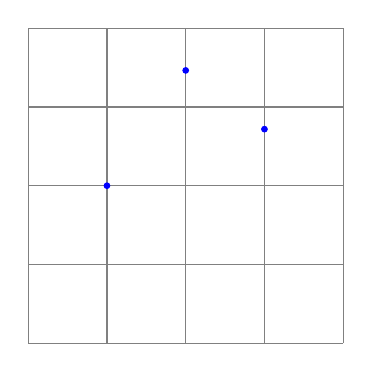
\begin{tikzpicture}[scale=1]
  \tkzInit[xmax=4,ymax=4]
  \tkzGrid
  \tkzDefPoint(-1+2,sqrt(4)){O}
  \tkzDefPoint({3*ln(exp(1))},{exp(1)}){A}
  \tkzDefPoint({4*sin(pi/6)},{4*cos(pi/6)}){B}
  \tkzDrawPoints[color=blue](O,B,A)
\end{tikzpicture}
\end{tkzexample}


\subsubsection{Polar coordinates }

\begin{tkzexample}[latex=7cm,small]
  \begin{tikzpicture}
  \foreach \an [count=\i] in {0,60,...,300}
   { \tkzDefPoint(\an:3){A_\i}}
  \tkzDrawPolygon(A_1,A_...,A_6)
  \tkzDrawPoints(A_1,A_...,A_6)
  \end{tikzpicture}
\end{tkzexample}

\subsubsection{Calculations and coordinates}
You must follow the syntax of \tkzNamePack{xfp} here. It is always possible to go through \tkzNamePack{pgfmath} but in this case, the coordinates must be calculated before using the macro \tkzcname{tkzDefPoint}.

\begin{tkzexample}[latex=6cm,small]
  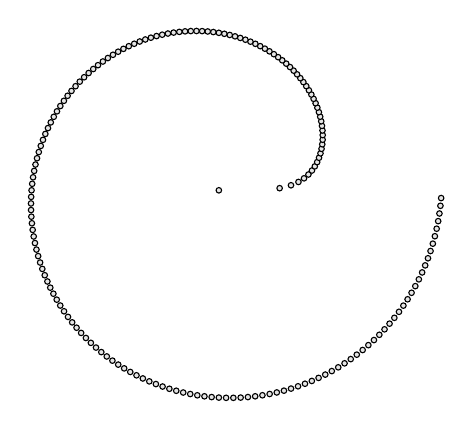
\begin{tikzpicture}[scale=.5]
  \foreach \an [count=\i] in {0,2,...,358}
   { \tkzDefPoint(\an:sqrt(sqrt(\an mm))){A_\i}}
   \tkzDrawPoints(A_1,A_...,A_180)
  \end{tikzpicture}
\end{tkzexample}


\subsubsection{Relative points}
First, we can use the \tkzNameEnv{scope} environment from \TIKZ.
In the following example, we have a way to define an equilateral triangle.

\begin{tkzexample}[latex=7cm,small]
\begin{tikzpicture}[scale=1]
  \tkzSetUpLine[color=blue!60]
 \begin{scope}[rotate=30]
  \tkzDefPoint(2,3){A}
  \begin{scope}[shift=(A)]
     \tkzDefPoint(90:5){B}
     \tkzDefPoint(30:5){C}
  \end{scope}
 \end{scope}
 \tkzDrawPolygon(A,B,C)
\tkzLabelPoints[above](B,C)
\tkzLabelPoints[below](A)
\tkzDrawPoints(A,B,C)
\end{tikzpicture}
\end{tkzexample}

%<--------------------------------------------------------------------------->
\subsection{Point relative to another: \tkzcname{tkzDefShiftPoint}}
\begin{NewMacroBox}{tkzDefShiftPoint}{\oarg{Point}\parg{$x,y$}\marg{name} or \parg{$\alpha$:$d$}\marg{name}}%
\begin{tabular}{lll}%
arguments &  default & definition \\
\midrule
\TAline{($x,y$)}{no default}{$x$ and $y$ are two dimensions, by default in cm.}
\TAline{($\alpha$:$d$)}{no default}{$\alpha$ is an angle in degrees, $d$ is a dimension}

\midrule
options &  default & definition \\

\midrule
\TOline{[pt]} {no default} {\tkzcname{tkzDefShiftPoint}[A](0:4)\{B\}}
\end{tabular}
\end{NewMacroBox}

\subsubsection{Isosceles triangle with  \tkzcname{tkzDefShiftPoint}}
This macro allows you to place one point relative to another. This is equivalent to a translation. Here is how to construct an isosceles triangle with main vertex $A$ and angle at vertex of $30^{\circ} $.

\begin{tkzexample}[latex=7cm,small]
\begin{tikzpicture}[rotate=-30]
 \tkzDefPoint(2,3){A}
 \tkzDefShiftPoint[A](0:4){B}
 \tkzDefShiftPoint[A](30:4){C}
 \tkzDrawSegments(A,B B,C C,A)
 \tkzMarkSegments[mark=|,color=red](A,B A,C)
 \tkzDrawPoints(A,B,C)
 \tkzLabelPoints(B,C)
 \tkzLabelPoints[above left](A)
\end{tikzpicture}
\end{tkzexample}

\subsubsection{Equilateral triangle}
Let's see how to get an equilateral triangle (there is much simpler)

\begin{tkzexample}[latex=7cm,small]
\begin{tikzpicture}[scale=1]
 \tkzDefPoint(2,3){A}
 \tkzDefShiftPoint[A](30:3){B}
 \tkzDefShiftPoint[A](-30:3){C}
 \tkzDrawPolygon(A,B,C)
 \tkzDrawPoints(A,B,C)
 \tkzLabelPoints(B,C)
 \tkzLabelPoints[above left](A)
 \tkzMarkSegments[mark=|,color=red](A,B A,C B,C)
\end{tikzpicture}
\end{tkzexample}

\subsubsection{Parallelogram}
There's a simpler way
\begin{tkzexample}[latex=7cm,small]
\begin{tikzpicture}
 \tkzDefPoint(0,0){A}
 \tkzDefPoint(30:3){B}
 \tkzDefShiftPointCoord[B](10:2){C}
 \tkzDefShiftPointCoord[A](10:2){D}
 \tkzDrawPolygon(A,...,D)
 \tkzDrawPoints(A,...,D)
\end{tikzpicture}
\end{tkzexample}

%<--------------------------------------------------------------------------->
\subsection{Definition of multiple points: \tkzcname{tkzDefPoints}}

\begin{NewMacroBox}{tkzDefPoints}{\oarg{local options}\marg{$x_1/y_1/n_1,x_2/y_2/n_2$, ...}}%
$x_i$ and $y_i$ are the coordinates of a referenced point $n_i$

\begin{tabular}{lll}%
\toprule
arguments &  default  & example  \\
\midrule
\TAline{$x_i/y_i/n_i$}{}{\tkzcname{tkzDefPoints\{0/0/O,2/2/A\}}}
\end{tabular}

\medskip
\begin{tabular}{lll}%
options             & default & definition   \\
\midrule
\TOline{shift} {no default} {Adds $(x,y)$ or $(\alpha:d)$ to all coordinates}
\end{tabular}
\end{NewMacroBox}

\subsection{Create a triangle}
\begin{tkzexample}[latex=6cm,small]
\begin{tikzpicture}[scale=1]
 \tkzDefPoints{0/0/A,4/0/B,4/3/C}
 \tkzDrawPolygon(A,B,C)
 \tkzDrawPoints(A,B,C)
\end{tikzpicture}
\end{tkzexample}

\subsection{Create a square}
Note here the syntax for drawing the polygon.
\begin{tkzexample}[latex=6cm,small]
\begin{tikzpicture}[scale=1]
 \tkzDefPoints{0/0/A,2/0/B,2/2/C,0/2/D}
 \tkzDrawPolygon(A,...,D)
 \tkzDrawPoints(A,B,C,D)
\end{tikzpicture}
\end{tkzexample}

\section{Special points}
The introduction of the dots was done in \tkzname{tkz-base}, the most important macro being \tkzcname{tkzDefPoint}. Here are some special points.
%<--------------------------------------------------------------------------->
\subsection{Middle of a segment \tkzcname{tkzDefMidPoint}}
It is a question of determining the middle of a segment.

\begin{NewMacroBox}{tkzDefMidPoint}{\parg{pt1,pt2}}%
The result is in \tkzname{tkzPointResult}. We can access it with \tkzcname{tkzGetPoint}.

 \medskip
\begin{tabular}{lll}%
\toprule
arguments & default & definition \\
\midrule
\TAline{(pt1,pt2)}{no default}{pt1 and pt2 are two points}
\end{tabular}
\end{NewMacroBox}

\subsubsection{Use of \tkzcname{tkzDefMidPoint}}
Review the use of \tkzcname{tkzDefPoint} in \tkzNamePack{tkz-base}.
\begin{tkzexample}[latex=7cm,small]
\begin{tikzpicture}[scale=1]
 \tkzDefPoint(2,3){A}
 \tkzDefPoint(4,0){B}
 \tkzDefMidPoint(A,B) \tkzGetPoint{C}
 \tkzDrawSegment(A,B)
 \tkzDrawPoints(A,B,C)
 \tkzLabelPoints[right](A,B,C)
\end{tikzpicture}
\end{tkzexample}

\subsection{Barycentric coordinates }

$pt_1$, $pt_2$, \dots, $pt_n$ being $n$ points, they define $n$ vectors $\overrightarrow{v_1}$, $\overrightarrow{v_2}$, \dots, $\overrightarrow{v_n}$ with the origin of the referential as the common endpoint. $\alpha_1$, $\alpha_2$,
\dots $\alpha_n$ are $n$ numbers, the vector obtained by:
\begin{align*}
  \frac{\alpha_1 \overrightarrow{v_1} + \alpha_2 \overrightarrow{v_2} + \cdots + \alpha_n \overrightarrow{v_n}}{\alpha_1
    + \alpha_2 + \cdots + \alpha_n}
\end{align*}
defines a single point.

\begin{NewMacroBox}{tkzDefBarycentricPoint}{\parg{pt1=$\alpha_1$,pt2=$\alpha_2$,\dots}}%
\begin{tabular}{lll}%
arguments & default & definition \\
\midrule
\TAline{(pt1=$\alpha_1$,pt2=$\alpha_2$,\dots)}{no default}{Each point has a assigned weight}
\bottomrule
\end{tabular}

\medskip
You need at least two points.
\end{NewMacroBox}


\subsubsection{Using \tkzcname{tkzDefBarycentricPoint} with two points}
In the following example, we obtain the barycentre of points $A$ and $B$ with coefficients $1$ and $2$, in other words:
\[
  \overrightarrow{AI}= \frac{2}{3}\overrightarrow{AB}
\]

\begin{tkzexample}[latex=7cm,small]
\begin{tikzpicture}
  \tkzDefPoint(2,3){A}
  \tkzDefShiftPointCoord[2,3](30:4){B}
  \tkzDefBarycentricPoint(A=1,B=2)
  \tkzGetPoint{I}
  \tkzDrawPoints(A,B,I)
  \tkzDrawLine(A,B)
  \tkzLabelPoints(A,B,I)
\end{tikzpicture}
\end{tkzexample}

\subsubsection{Using \tkzcname{tkzDefBarycentricPoint} with three points}
This time $M$ is simply the centre of gravity of the triangle. For reasons of simplification and homogeneity, there is also \tkzcname{tkzCentroid}.
\begin{tkzexample}[latex=7cm,small]
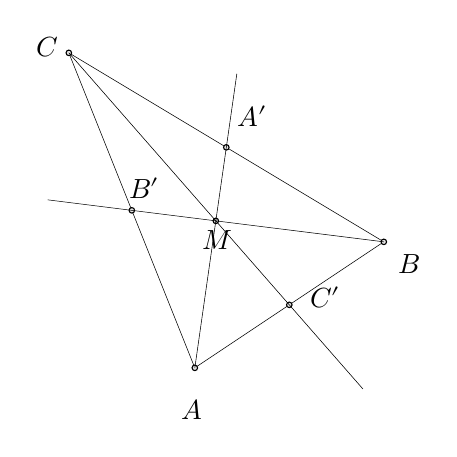
\begin{tikzpicture}[scale=.8]
  \tkzDefPoint(2,1){A}
  \tkzDefPoint(5,3){B}
  \tkzDefPoint(0,6){C}
  \tkzDefBarycentricPoint(A=1,B=1,C=1)
  \tkzGetPoint{M}
  \tkzDefMidPoint(A,B)  \tkzGetPoint{C'}
  \tkzDefMidPoint(A,C)  \tkzGetPoint{B'}
  \tkzDefMidPoint(C,B)  \tkzGetPoint{A'}
  \tkzDrawPolygon(A,B,C)
  \tkzDrawPoints(A',B',C')
  \tkzDrawPoints(A,B,C,M)
  \tkzDrawLines[add=0 and 1](A,M B,M C,M)
  \tkzLabelPoint(M){$M$}
  \tkzAutoLabelPoints[center=M](A,B,C)
  \tkzAutoLabelPoints[center=M,above right](A',B',C')
\end{tikzpicture}
\end{tkzexample}

\subsection{Internal Similitude Center}
The centres of the two homotheties in which two circles correspond are called external and internal centres of similitude.

\begin{tkzexample}[latex=6cm,small]
\begin{tikzpicture}[scale=.75,rotate=-30]
 \tkzDefPoint(0,0){O}
 \tkzDefPoint(4,-5){A}
 \tkzDefIntSimilitudeCenter(O,3)(A,1)
 \tkzGetPoint{I}
 \tkzExtSimilitudeCenter(O,3)(A,1)
 \tkzGetPoint{J}
 \tkzDefTangent[from with R= I](O,3 cm)
 \tkzGetPoints{D}{E}
 \tkzDefTangent[from with R= I](A,1 cm)
 \tkzGetPoints{D'}{E'}
 \tkzDefTangent[from  with R= J](O,3 cm)
 \tkzGetPoints{F}{G}
 \tkzDefTangent[from with R= J](A,1 cm)
 \tkzGetPoints{F'}{G'}
 \tkzDrawCircle[R,fill=red!50,opacity=.3](O,3 cm)
 \tkzDrawCircle[R,fill=blue!50,opacity=.3](A,1 cm)
 \tkzDrawSegments[add = .5 and .5,color=red](D,D' E,E')
 \tkzDrawSegments[add= 0 and 0.25,color=blue](J,F J,G)
 \tkzDrawPoints(O,A,I,J,D,E,F,G,D',E',F',G')
 \tkzLabelPoints[font=\scriptsize](O,A,I,J,D,E,F,G,D',E',F',G')
\end{tikzpicture}
\end{tkzexample}

\endinput



\section{Special points relating to a triangle}

\subsection{Triangle center: \tkzcname{tkzDefTriangleCenter}}

This macro allows you to define the center of a triangle.


\begin{NewMacroBox}{tkzDefTriangleCenter}{\oarg{local options}\parg{A,B,C}}%
\tkzHandBomb\ Be careful, the arguments are lists of three points. This macro is used in conjunction with \tkzcname{tkzGetPoint} to get the center you are looking for. You can use \tkzname{tkzPointResult} if it is not necessary to keep the results.

\medskip
\begin{tabular}{lll}%
\toprule
arguments & default & definition \\

\midrule
\TAline{(pt1,pt2,pt3)}{no default}{three points}
\midrule
options             & default & definition                         \\
\midrule
\TOline{ortho}  {circum}{intersection of the altitudes of a triangle}
\TOline{centroid} {circum}{centre of gravity. Intersection of the medians }
\TOline{circum}{circum}{circle center circumscribed}
\TOline{in}    {circum}{center of the circle inscribed in a triangle }
\TOline{ex}    {circum}{center of a circle exinscribed to a triangle }
\TOline{euler}{circum}{center of Euler's circle }
\TOline{symmedian} {circum}{Lemoine's point or symmedian centre or Grebe's point }
\TOline{spieker} {circum}{Spieker Circle Center}
\TOline{nagel}{circum}{Nagel Center}
\TOline{mittenpunkt} {circum}{also called the middlespoint}
\TOline{feuerbach}{circum}{Feuerbach Point}

\end{tabular}
\end{NewMacroBox}

\subsubsection{Option \tkzname{ortho} or \tkzname{orthic}}
 The intersection $H$ of the three altitudes  of a triangle is called the orthocenter.

\begin{tkzexample}[latex=5cm,small]
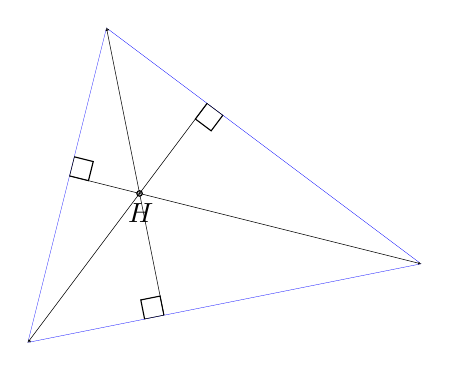
\begin{tikzpicture}
  \tkzDefPoint(0,0){A}
  \tkzDefPoint(5,1){B}
  \tkzDefPoint(1,4){C}
  \tkzClipPolygon(A,B,C)
  \tkzDefTriangleCenter[ortho](B,C,A)
    \tkzGetPoint{H}
  \tkzDefSpcTriangle[orthic,name=H](A,B,C){a,b,c}
  \tkzDrawPolygon[color=blue](A,B,C)
  \tkzDrawPoints(A,B,C,H)
  \tkzDrawLines[add=0 and 1](A,Ha B,Hb C,Hc)
  \tkzLabelPoint(H){$H$}
  \tkzAutoLabelPoints[center=H](A,B,C)
  \tkzMarkRightAngles(A,Ha,B B,Hb,C C,Hc,A)
\end{tikzpicture}
\end{tkzexample}

\subsubsection{Option \tkzname{centroid}}
\begin{tkzexample}[latex=5cm,small]
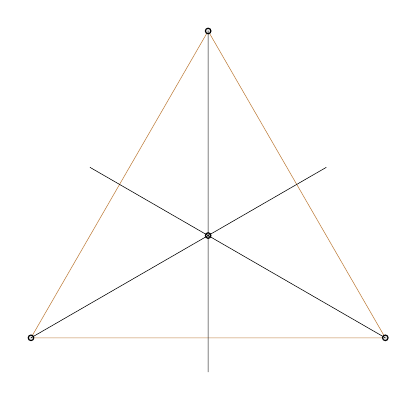
\begin{tikzpicture}[scale=.75]
  \tkzDefPoints{-1/1/A,5/1/B}
  \tkzDefEquilateral(A,B)
  \tkzGetPoint{C}
  \tkzDefTriangleCenter[centroid](A,B,C)
      \tkzGetPoint{G}
  \tkzDrawPolygon[color=brown](A,B,C)
  \tkzDrawPoints(A,B,C,G)
  \tkzDrawLines[add = 0 and 2/3](A,G B,G C,G)
\end{tikzpicture}
\end{tkzexample}

\subsubsection{Option \tkzname{circum}}
\begin{tkzexample}[latex=6cm,small]
 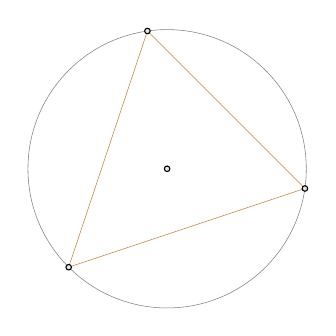
\begin{tikzpicture}
  \tkzDefPoints{0/1/A,3/2/B,1/4/C}
  \tkzDefTriangleCenter[circum](A,B,C)
  \tkzGetPoint{G}
  \tkzDrawPolygon[color=brown](A,B,C)
  \tkzDrawCircle(G,A)
  \tkzDrawPoints(A,B,C,G)
 \end{tikzpicture}
\end{tkzexample}

\subsubsection{Option \tkzname{in}}
In geometry, the incircle or inscribed circle of a triangle is the largest circle contained in the triangle; it touches (is tangent to) the three sides. The center of the incircle is a triangle center called the triangle's incenter.
The center of the incircle, called the incenter, can be found as the intersection of the three internal angle bisectors. The center of an excircle is the intersection of the internal bisector of one angle (at vertex $A$, for example) and the external bisectors of the other two. The center of this excircle is called the excenter relative to the vertex $A$, or the excenter of $A$. Because the internal bisector of an angle is perpendicular to its external bisector, it follows that the center of the incircle together with the three excircle centers form an orthocentric system.(\url{https://en.wikipedia.org/wiki/Incircle_and_excircles_of_a_triangle})
 
 \medskip
 We get the centre of the inscribed circle of the triangle. The result is of course in \tkzname{tkzPointResult}. We can retrieve it with \tkzcname{tkzGetPoint}.

\begin{tkzexample}[latex=6cm,small]
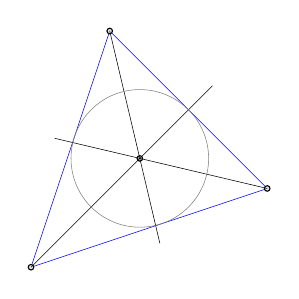
\begin{tikzpicture}
  \tkzDefPoints{0/1/A,3/2/B,1/4/C}
  \tkzDefTriangleCenter[in](A,B,C)\tkzGetPoint{I}
  \tkzDefPointBy[projection=onto A--C](I)
  \tkzGetPoint{Ib}
  \tkzDrawPolygon[color=blue](A,B,C)
  \tkzDrawPoints(A,B,C,I)
  \tkzDrawLines[add = 0 and 2/3](A,I B,I C,I)
  \tkzDrawCircle(I,Ib)
\end{tikzpicture}
\end{tkzexample}

\subsubsection{Option \tkzname{ex}}
An excircle or escribed circle of the triangle is a circle lying outside the triangle, tangent to one of its sides and tangent to the extensions of the other two. Every triangle has three distinct excircles, each tangent to one of the triangle's sides.
(\url{https://en.wikipedia.org/wiki/Incircle_and_excircles_of_a_triangle})


 We get the centre of an inscribed circle of the triangle. The result is of course in \tkzname{tkzPointResult}. We can retrieve it with \tkzcname{tkzGetPoint}.

\begin{tkzexample}[latex=8cm,small]
  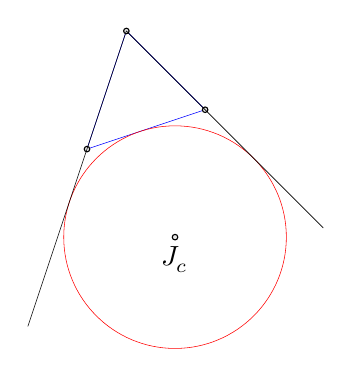
\begin{tikzpicture}[scale=.5]
    \tkzDefPoints{0/1/A,3/2/B,1/4/C}
    \tkzDefTriangleCenter[ex](B,C,A)
    \tkzGetPoint{J_c}
    \tkzDefPointBy[projection=onto A--B](J_c)
    \tkzGetPoint{Tc}
    %or
    % \tkzDefCircle[ex](B,C,A)
    % \tkzGetFirstPoint{J_c}
    % \tkzGetSecondPoint{Tc}
    \tkzDrawPolygon[color=blue](A,B,C)
    \tkzDrawPoints(A,B,C,J_c)
    \tkzDrawCircle[red](J_c,Tc)
    \tkzDrawLines[add=1.5 and 0](A,C B,C)
    \tkzLabelPoints(J_c)
  \end{tikzpicture}
\end{tkzexample}

\subsubsection{Option \tkzname{euler}}
This macro allows to obtain the center of the circle of the nine points or euler's circle or Feuerbach's circle.
The nine-point circle, also called Euler's circle or the Feuerbach circle, is the circle that passes through the perpendicular feet $H_A$, $H_B$, and $H_C$ dropped from the vertices of any reference triangle $ABC$ on the sides opposite them. Euler showed in 1765 that it also passes through the midpoints $M_A$, $M_B$, $M_C$ of the sides of $ABC$. By Feuerbach's theorem, the nine-point circle also passes through the midpoints $E_A$, $E_B$, and $E_C$ of the segments that join the vertices and the orthocenter $H$. These points are commonly referred to as the Euler points. (\url{http://mathworld.wolfram.com/Nine-PointCircle.html})

\begin{tkzexample}[latex=7cm,small]
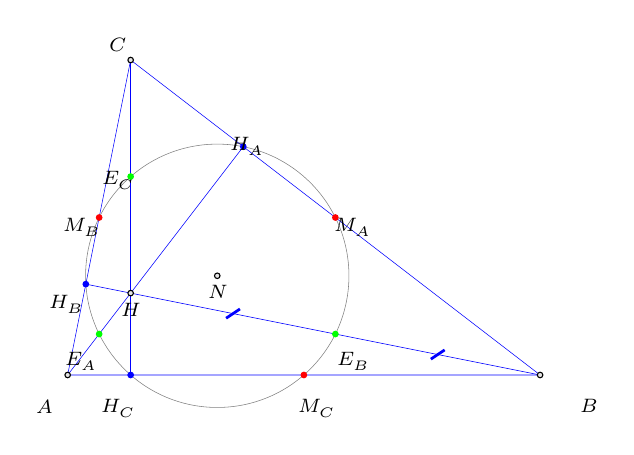
\begin{tikzpicture}[scale=1]
 \tkzDefPoints{0/0/A,6/0/B,0.8/4/C}
 \tkzDefSpcTriangle[medial,
     name=M](A,B,C){_A,_B,_C}
 \tkzDefTriangleCenter[euler](A,B,C)
    \tkzGetPoint{N} % I= N nine points
 \tkzDefTriangleCenter[ortho](A,B,C)
    \tkzGetPoint{H}
 \tkzDefMidPoint(A,H) \tkzGetPoint{E_A}
 \tkzDefMidPoint(C,H) \tkzGetPoint{E_C}
 \tkzDefMidPoint(B,H) \tkzGetPoint{E_B}
 \tkzDefSpcTriangle[ortho,name=H](A,B,C){_A,_B,_C}
 \tkzDrawPolygon[color=blue](A,B,C)
 \tkzDrawCircle(N,E_A)
 \tkzDrawSegments[blue](A,H_A B,H_B C,H_C)
 \tkzDrawPoints(A,B,C,N,H)
 \tkzDrawPoints[red](M_A,M_B,M_C)
 \tkzDrawPoints[blue]( H_A,H_B,H_C)
 \tkzDrawPoints[green](E_A,E_B,E_C)
 \tkzAutoLabelPoints[center=N,
  font=\scriptsize](A,B,C,%
   M_A,M_B,M_C,%
   H_A,H_B,H_C,%
   E_A,E_B,E_C)
 \tkzLabelPoints[font=\scriptsize](H,N)
 \tkzMarkSegments[mark=s|,size=3pt,
     color=blue,line width=1pt](B,E_B E_B,H)
\end{tikzpicture}
\end{tkzexample}


\subsubsection{Option \tkzname{symmedian}}

\begin{tkzexample}[latex=6cm,small]
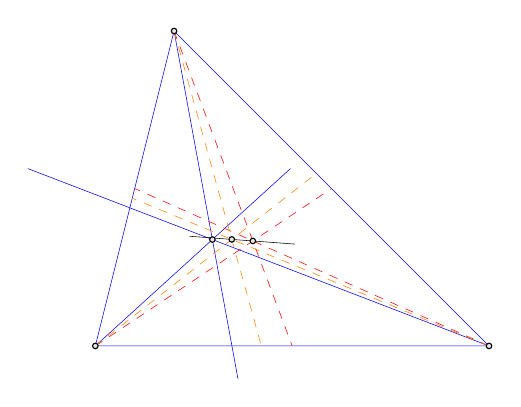
\begin{tikzpicture}
  \tkzDefPoint(0,0){A}
  \tkzDefPoint(5,0){B}
  \tkzDefPoint(1,4){C}
  \tkzDefTriangleCenter[symmedian](A,B,C)\tkzGetPoint{K}
  \tkzDefTriangleCenter[median](A,B,C)\tkzGetPoint{G}
  \tkzDefTriangleCenter[in](A,B,C)\tkzGetPoint{I}
  \tkzDefSpcTriangle[centroid,name=M](A,B,C){a,b,c}
  \tkzDefSpcTriangle[incentral,name=I](A,B,C){a,b,c}
  \tkzDrawPolygon[color=blue](A,B,C)
  \tkzDrawLines[add = 0 and 2/3,blue](A,K B,K C,K)
  \tkzDrawSegments[red,dashed](A,Ma B,Mb C,Mc)
  \tkzDrawSegments[orange,dashed](A,Ia B,Ib C,Ic)
  \tkzDrawLine[add=2 and 2](G,I)
  \tkzDrawPoints(A,B,C,K,G,I)
\end{tikzpicture}
\end{tkzexample}


\subsubsection{Option \tkzname{nagel}}
Let $Ta$ be the point at which the excircle with center $Ja$ meets the side $BC$ of a triangle $ABC$, and define $Tb$ and $Tc$ similarly. Then the lines $ATa$, $BTb$, and $CTc$ concur in the Nagel point $Na$.
\href{http://mathworld.wolfram.com/NagelPoint.html}{Weisstein, Eric W. "Nagel point." From MathWorld--A Wolfram Web Resource. }


\begin{tkzexample}[latex=8cm,small]
  \begin{tikzpicture}[scale=.5]
  \tkzDefPoints{0/0/A,6/0/B,4/6/C}
  \tkzDefSpcTriangle[ex](A,B,C){Ja,Jb,Jc}
  \tkzDefSpcTriangle[extouch](A,B,C){Ta,Tb,Tc}
  \tkzDrawPoints(Ja,Jb,Jc,Ta,Tb,Tc)
  \tkzLabelPoints(Ja,Jb,Jc,Ta,Tb,Tc)
  \tkzDrawPolygon[blue](A,B,C)
  \tkzDefTriangleCenter[nagel](A,B,C) \tkzGetPoint{Na}
  \tkzDrawPoints[blue](B,C,A)
  \tkzDrawPoints[red](Na)
  \tkzLabelPoints[blue](B,C,A)
  \tkzLabelPoints[red](Na)
  \tkzDrawLines[add=0 and 1](A,Ta B,Tb C,Tc)
  \tkzShowBB\tkzClipBB
  \tkzDrawLines[add=1 and 1,dashed](A,B B,C C,A)
  \tkzDrawCircles[ex,gray](A,B,C C,A,B B,C,A)
  \tkzDrawSegments[dashed](Ja,Ta Jb,Tb Jc,Tc)
  \tkzMarkRightAngles[fill=gray!20](Ja,Ta,C
              Jb,Tb,A Jc,Tc,B)
  \end{tikzpicture}
\end{tkzexample}


\subsubsection{Option   \tkzname{mittenpunkt}} 
\begin{tkzexample}[latex=8cm,small]
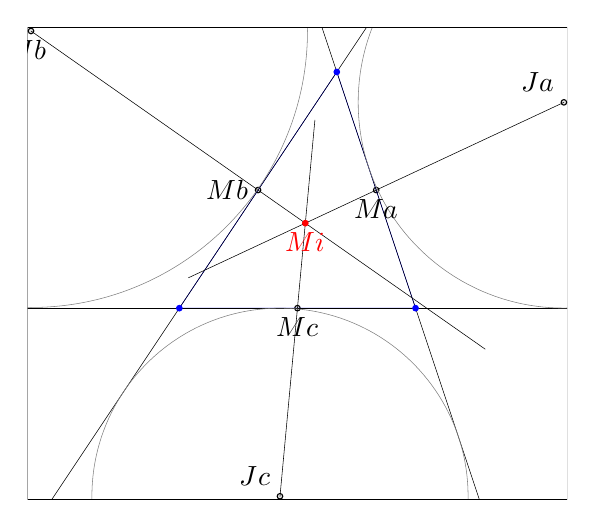
\begin{tikzpicture}[scale=.5]
 \tkzDefPoints{0/0/A,6/0/B,4/6/C}
 \tkzDefSpcTriangle[centroid](A,B,C){Ma,Mb,Mc}
 \tkzDefSpcTriangle[ex](A,B,C){Ja,Jb,Jc}
 \tkzDefSpcTriangle[extouch](A,B,C){Ta,Tb,Tc}
 \tkzDefTriangleCenter[mittenpunkt](A,B,C) 
 \tkzGetPoint{Mi}
 \tkzDrawPoints(Ma,Mb,Mc,Ja,Jb,Jc)
 \tkzClipBB
 \tkzDrawPolygon[blue](A,B,C)
 \tkzDrawLines[add=0 and 1](Ja,Ma 
               Jb,Mb Jc,Mc)
 \tkzDrawLines[add=1 and 1](A,B A,C B,C)
 \tkzDrawCircles[gray](Ja,Ta Jb,Tb Jc,Tc)
 \tkzDrawPoints[blue](B,C,A)
 \tkzDrawPoints[red](Mi)
 \tkzLabelPoints[red](Mi)
 \tkzLabelPoints[left](Mb)
 \tkzLabelPoints(Ma,Mc,Jb,Jc)
 \tkzLabelPoints[above left](Ja,Jc)
 \tkzShowBB
\end{tikzpicture}
\end{tkzexample}
%<---------------------------------------------------------------------->
%<---------------------------------------------------------------------->
\section{Draw a point}
\subsubsection{Drawing points \tkzcname{tkzDrawPoint}} \hypertarget{tdrp}{}

\begin{NewMacroBox}{tkzDrawPoint}{\oarg{local options}\parg{name}}%
\begin{tabular}{lll}%
arguments &  default & definition                 \\
\midrule
\TAline{name of point} {no default}  {Only one point name is accepted}
\bottomrule
\end{tabular}

\medskip
The argument is required. The disc takes the color of the circle, but  lighter. It is possible to change everything. The point is a node and therefore it is invariant if the drawing is modified by scaling.

\medskip
\begin{tabular}{lll}%
\toprule
options             & default & definition \\
\midrule
\TOline{shape}  {circle}{Possible \tkzname{cross} or \tkzname{cross out}}
\TOline{size}  {6}{$6 \times$ \tkzcname{pgflinewidth}}
\TOline{color}  {black}{the default color can be changed }
\bottomrule
\end{tabular}

\medskip
{We can create other forms such as \tkzname{cross}}
\end{NewMacroBox}

\subsubsection{Example of point drawings}
Note that \tkzname{scale} does not affect the shape of the dots. Which is normal.  Most of the time, we are satisfied with a single point shape that we can define from the beginning, either with a macro or by modifying a configuration file.


\begin{tkzexample}[latex=5cm,small]
  \begin{tikzpicture}[scale=.5]
   \tkzDefPoint(1,3){A}
   \tkzDefPoint(4,1){B}
   \tkzDefPoint(0,0){O}
   \tkzDrawPoint[color=red](A)
   \tkzDrawPoint[fill=blue!20,draw=blue](B)
   \tkzDrawPoint[color=green](O)
  \end{tikzpicture}
\end{tkzexample}

It is possible to draw several points at once but this macro is a little slower than the previous one. Moreover, we have to make do with the same options for all the points.

\hypertarget{tdrps}{}
\begin{NewMacroBox}{tkzDrawPoints}{\oarg{local options}\parg{liste}}%
\begin{tabular}{lll}%
arguments &  default  & definition \\
\midrule
\TAline{points list}{no default}{example \tkzcname{tkzDrawPoints(A,B,C)}}
\bottomrule
\end{tabular}

\medskip
\begin{tabular}{lll}%
options             & default & definition \\
\midrule
\TOline{shape}  {circle}{Possible \tkzname{cross} or \tkzname{cross out}}
\TOline{size}  {6}{$6 \times$ \tkzcname{pgflinewidth}}
\TOline{color}  {black}{the default color can be changed }
\bottomrule
\end{tabular}

\medskip
\tkzHandBomb\ Beware of the final "s", an oversight leads to cascading errors if you try to draw multiple points. The options are the same as for the previous macro.
\end{NewMacroBox}

\subsubsection{First example}

\begin{tkzexample}[latex=7cm,small]
\begin{tikzpicture}
  \tkzDefPoint(1,3){A} 
  \tkzDefPoint(4,1){B} 
  \tkzDefPoint(0,0){C} 
  \tkzDrawPoints[size=6,color=red,
               fill=red!50](A,B,C)
\end{tikzpicture}
\end{tkzexample}

\subsubsection{Second example}

\begin{tkzexample}[latex=7cm,small]
\begin{tikzpicture}[scale=.5]
 \tkzDefPoint(2,3){A}  \tkzDefPoint(5,-1){B}
 \tkzDefPoint[label=below:$\mathcal{C}$,
               shift={(2,3)}](-30:5.5){E}
 \begin{scope}[shift=(A)]
    \tkzDefPoint(30:5){C}
 \end{scope}
 \tkzCalcLength[cm](A,B)\tkzGetLength{rAB}
 \tkzDrawCircle[R](A,\rAB cm)
 \tkzDrawSegment(A,B)
 \tkzDrawPoints(A,B,C)
 \tkzLabelPoints(B,C)
 \tkzLabelPoints[above](A)
\end{tikzpicture}
\end{tkzexample}

\section{Point on line or circle}
\subsection{Point on a line}

\begin{NewMacroBox}{tkzDefPointOnLine}{\oarg{local options}\parg{A,B}}%
\begin{tabular}{lll}%
arguments &  default & definition                 \\
\midrule
\TAline{pt1,pt2} {no default}  {Two points to define a line}
\bottomrule
\end{tabular}

\medskip
\begin{tabular}{lll}%
options       & default & definition \\
\midrule
\TOline{pos=nb}  {}{nb is a decimal  }
\end{tabular}
\end{NewMacroBox}

\subsubsection{Use of option \tkzname{pos}}
\begin{tkzexample}[latex=9cm,small]
  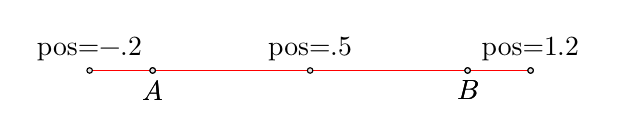
\begin{tikzpicture}
  \tkzDefPoints{0/0/A,4/0/B}
  \tkzDrawLine[red](A,B)
  \tkzDefPointOnLine[pos=1.2](A,B) 
  \tkzGetPoint{P}
  \tkzDefPointOnLine[pos=-0.2](A,B) 
  \tkzGetPoint{R}
  \tkzDefPointOnLine[pos=0.5](A,B) 
  \tkzGetPoint{S}
  \tkzDrawPoints(A,B,P)
  \tkzLabelPoints(A,B)
  \tkzLabelPoint[above](P){pos=$1.2$}
  \tkzLabelPoint[above](R){pos=$-.2$}
  \tkzLabelPoint[above](S){pos=$.5$}
  \tkzDrawPoints(A,B,P,R,S)
  \tkzLabelPoints(A,B)
  \end{tikzpicture}
\end{tkzexample}

\subsection{Point on a circle}

\begin{NewMacroBox}{tkzDefPointOnCircle}{\oarg{local options}}%
\begin{tabular}{lll}%
options   & default & definition \\
\midrule
\TOline{angle}  {0}{angle formed with the abscissa axis}
\TOline{center}  {|tkzPointResult|}{circle center required}
\TOline{radius}  {|\BS tkzLengthResult|}{radius circle}
\end{tabular}
\end{NewMacroBox}

\begin{tkzexample}[latex=7cm,small]
\begin{tikzpicture}
 \tkzDefPoints{0/0/A,4/0/B,0.8/3/C}  
 \tkzDefPointOnCircle[angle=90,center=B,radius=1 cm]
 \tkzGetPoint{I}    
 \tkzDefCircle[circum](A,B,C)
 \tkzGetPoint{G} \tkzGetLength{rG}
 \tkzDefPointOnCircle[angle=30,center=G,radius=\rG pt]
 \tkzGetPoint{J}
 \tkzDrawCircle[R,teal](B,1cm) 
 \tkzDrawPoint[teal](I)
 \tkzDrawPoints(A,B,C)
 \tkzDrawCircle(G,J)
 \tkzDrawPoints(G,J)
 \tkzDrawPoint[red](J)
 \tkzLabelPoints(G,J)
\end{tikzpicture}
\end{tkzexample}
\endinput
\section{Definition of points by transformation; \tkzcname{tkzDefPointBy} }
These transformations are:

\begin{itemize}
   \item translation;
   \item homothety;
   \item orthogonal reflection or symmetry;
   \item central symmetry;
   \item orthogonal projection;
   \item rotation (degrees or radians);
   \item inversion with respect to a circle.
\end{itemize}

The choice of transformations is made through the options. There are two macros, one for the transformation of a single point \tkzcname{tkzDefPointBy} and the other for the transformation of a list of points \tkzcname{tkzDefPointsBy}. By default the image of $A$ is $A'$. For example, we'll write:
\begin{tkzltxexample}[]
\tkzDefPointBy[translation= from A to A'](B)
\end{tkzltxexample}
The result is in \tkzname{tkzPointResult}
\medskip
\begin{NewMacroBox}{tkzDefPointBy}{\oarg{local options}\parg{pt}}%
The argument is a simple existing point and its image is stored in \tkzname{tkzPointResult}. If you want to keep this point then the macro \tkzcname{tkzGetPoint\{M\}} allows you to assign the name \tkzname{M} to the point.

\begin{tabular}{lll}%
\toprule
arguments &  definition & examples               \\
\midrule
\TAline{pt}   {existing point name}   {$(A)$}
\bottomrule
\end{tabular}

\begin{tabular}{lll}%
options     &     & examples                         \\
\midrule
\TOline{translation}{= from \#1 to \#2}{[translation=from A to B](E)}
\TOline{homothety}  {= center \#1 ratio \#2}{[homothety=center A ratio .5](E)}
\TOline{reflection} {= over \#1--\#2}{[reflection=over A--B](E)}
\TOline{symmetry }  {= center \#1}{[symmetry=center A](E)}
\TOline{projection }{= onto \#1--\#2}{[projection=onto A--B](E)}
\TOline{rotation }  {= center \#1 angle \#2}{[rotation=center O angle 30](E)}
\TOline{rotation in rad}{= center \#1 angle \#2}{[rotation in rad=center O angle pi/3](E)}
\TOline{inversion}{= center \#1 through \#2}{[inversion =center O through A](E)}
\bottomrule
\end{tabular}

The image is only defined and not drawn.
\end{NewMacroBox}

\subsection{Examples of transformations}
\subsubsection{Example of translation}

\subsection{Example of translation}
\begin{tkzexample}[latex=7cm,small]
\begin{tikzpicture}[>=latex]
 \tkzDefPoint(0,0){A}  \tkzDefPoint(3,1){B}
 \tkzDefPoint(3,0){C}
 \tkzDefPointBy[translation= from B to A](C)
 \tkzGetPoint{D}
 \tkzDrawPoints[teal](A,B,C,D)
 \tkzLabelPoints[color=teal](A,B,C,D)
 \tkzDrawSegments[orange,->](A,B D,C)
\end{tikzpicture}
\end{tkzexample}

\subsubsection{Example of reflection (orthogonal symmetry)}

\begin{tkzexample}[vbox,small]
\begin{tikzpicture}[scale=1]
 \tkzDefPoints{1.5/-1.5/C,-4.5/2/D}
 \tkzDefPoint(-4,-2){O}
 \tkzDefPoint(-2,-2){A}
 \foreach \i in {0,1,...,4}{%
 \pgfmathparse{0+\i * 72}
 \tkzDefPointBy[rotation=%
 center O angle \pgfmathresult](A)
  \tkzGetPoint{A\i}
 \tkzDefPointBy[reflection = over C--D](A\i)
  \tkzGetPoint{A\i'}}
 \tkzDrawPolygon(A0, A2, A4, A1, A3)
 \tkzDrawPolygon(A0', A2', A4', A1', A3')
 \tkzDrawLine[add= .5 and .5](C,D)
\end{tikzpicture}
\end{tkzexample}


\subsubsection{Example of \tkzname{homothety} and \tkzname{projection}}

\begin{tkzexample}[vbox,small]
\begin{tikzpicture}[scale=1.2]
  \tkzDefPoint(0,1){A}   \tkzDefPoint(5,3){B}   \tkzDefPoint(3,4){C}
  \tkzDefLine[bisector](B,A,C)                     \tkzGetPoint{a}
  \tkzDrawLine[add=0 and 0,color=magenta!50 ](A,a)
  \tkzDefPointBy[homothety=center A ratio .5](a)   \tkzGetPoint{a'}
  \tkzDefPointBy[projection = onto A--B](a')       \tkzGetPoint{k'}
  \tkzDefPointBy[projection = onto A--B](a)       \tkzGetPoint{k}
  \tkzDrawLines[add= 0 and .3](A,k A,C)
  \tkzDrawSegments[blue](a',k' a,k)
  \tkzDrawPoints(a,a',k,k',A)
  \tkzDrawCircles(a',k' a,k)
  \tkzLabelPoints(a,a',k,A)
\end{tikzpicture}
\end{tkzexample}


\subsubsection{Example of projection}
\begin{tkzexample}[vbox,small]
\begin{tikzpicture}[scale=1.5]
 \tkzDefPoint(0,0){A}
 \tkzDefPoint(0,4){B}
 \tkzDefTriangle[pythagore](B,A) \tkzGetPoint{C}
 \tkzDefLine[bisector](B,C,A) \tkzGetPoint{c}
 \tkzInterLL(C,c)(A,B)        \tkzGetPoint{D}
 \tkzDefPointBy[projection=onto B--C](D) \tkzGetPoint{G}
 \tkzInterLC(C,D)(D,A) \tkzGetPoints{E}{F}
 \tkzDrawPolygon[teal](A,B,C)
 \tkzDrawSegment(C,D)
 \tkzDrawCircle(D,A)
 \tkzDrawSegment[orange](D,G)
 \tkzMarkRightAngle[fill=orange!20](D,G,B)
 \tkzDrawPoints(A,C,F) \tkzLabelPoints(A,C,F)
 \tkzDrawPoints(B,D,E,G)
 \tkzLabelPoints[above right](B,D,E,G)
 \end{tikzpicture}
 \end{tkzexample}

\subsubsection{Example of symmetry}
\begin{tkzexample}[vbox,small]
\begin{tikzpicture}[scale=1]
  \tkzDefPoint(0,0){O}
  \tkzDefPoint(2,-1){A}
  \tkzDefPoint(2,2){B}
  \tkzDefPointsBy[symmetry=center O](B,A){}
  \tkzDrawLine(A,A')
  \tkzDrawLine(B,B')
  \tkzMarkAngle[mark=s,arc=lll,
      size=2 cm,mkcolor=red](A,O,B)
  \tkzLabelAngle[pos=1,circle,draw,
     fill=blue!10](A,O,B){$60^{\circ}$}
  \tkzDrawPoints(A,B,O,A',B')
  \tkzLabelPoints(A,B,O,A',B')
\end{tikzpicture}
\end{tkzexample}

\subsubsection{Example of rotation}
\begin{tkzexample}[latex=7cm,small]
\begin{tikzpicture}[scale=0.5]
 \tkzDefPoint(0,0){A}
 \tkzDefPoint(5,0){B}
 \tkzDrawSegment(A,B)
 \tkzDefPointBy[rotation=center A angle 60](B)
 \tkzGetPoint{C}
 \tkzDefPointBy[symmetry=center C](A)
 \tkzGetPoint{D}
 \tkzDrawSegment(A,tkzPointResult)
 \tkzDrawLine(B,D)
 \tkzDrawArc[orange,delta=10](A,B)(C)
 \tkzDrawArc[orange,delta=10](B,C)(A)
 \tkzDrawArc[orange,delta=10](C,D)(D)
 \tkzMarkRightAngle(D,B,A)
\end{tikzpicture}
\end{tkzexample}

\subsubsection{Example of rotation in radian}
\begin{tkzexample}[latex=6cm,small]
\begin{tikzpicture}
  \tkzDefPoint["$A$" left](1,5){A}
  \tkzDefPoint["$B$" right](5,2){B}
  \tkzDefPointBy[rotation in rad= center A angle pi/3](B)
  \tkzGetPoint{C}
  \tkzDrawSegment(A,B)
  \tkzDrawPoints(A,B,C)
  \tkzCompass[color=red](A,C)
  \tkzCompass[color=red](B,C)
  \tkzLabelPoints(C)
\end{tikzpicture}
\end{tkzexample}

\subsubsection{Inversion of points}
\begin{tkzexample}[latex=8cm,small]
\begin{tikzpicture}[scale=1.5]
  \tkzDefPoint(0,0){O}
  \tkzDefPoint(1,0){A}
  \tkzDefPoint(-1.5,-1.5){z1}
  \tkzDefPoint(0.35,0){z2}
  \tkzDefPointBy[inversion =%
      center O through A](z1)
  \tkzGetPoint{Z1}
  \tkzDefPointBy[inversion =%
      center O through A](z2)
  \tkzGetPoint{Z2}
  \tkzDrawCircle(O,A)
  \tkzDrawPoints[color=black,
      fill=red,size=4](Z1,Z2)
  \tkzDrawSegments(z1,Z1 z2,Z2)
  \tkzDrawPoints[color=black,
      fill=red,size=4](O,z1,z2)
  \tkzLabelPoints(O,A,z1,z2,Z1,Z2)
\end{tikzpicture}
\end{tkzexample}


\subsubsection{Point Inversion: Orthogonal Circles}
\begin{tkzexample}[latex=8cm,small]
\begin{tikzpicture}[scale=1.5]
  \tkzDefPoint(0,0){O}
  \tkzDefPoint(1,0){A}
  \tkzDrawCircle(O,A)
  \tkzDefPoint(0.5,-0.25){z1}
  \tkzDefPoint(-0.5,-0.5){z2}
  \tkzDefPointBy[inversion = %
     center O through A](z1)
  \tkzGetPoint{Z1}
  \tkzCircumCenter(z1,z2,Z1)
  \tkzGetPoint{c}
  \tkzDrawCircle(c,Z1)
  \tkzDrawPoints[color=black,
     fill=red,size=4](O,z1,z2,Z1,O,A)
\end{tikzpicture}
\end{tkzexample}

\subsection{Transformation of multiple points; \tkzcname{tkzDefPointsBy} }
Variant of the previous macro for defining multiple images.
You must give the names of the images as arguments, or indicate that the names of the images are formed from the names of the antecedents, leaving the argument empty.

\begin{tkzltxexample}[]
\tkzDefPointsBy[translation= from A to A'](B,C){}
\end{tkzltxexample}
The images are $B'$ and $C'$.

\begin{tkzltxexample}[]
\tkzDefPointsBy[translation= from A to A'](B,C){D,E}
\end{tkzltxexample}
The images are $D$ and $E$.

\begin{tkzltxexample}[]
\tkzDefPointsBy[translation= from A to A'](B)
\end{tkzltxexample}
The image is $B'$.
\begin{NewMacroBox}{tkzDefPointsBy}{\oarg{local options}\parg{list of points}\marg{list of points}}%
\begin{tabular}{lll}%
arguments &  examples  &                  \\
\midrule
\TAline{\parg{list of points}\marg{list of pts}}{(A,B)\{E,F\}}{$E$ is the image of $A$ and $F$ is the image of $B$.}   \\
\bottomrule
\end{tabular}

\medskip
If the list of images is empty then the name of the image is the name of the antecedent to which " ' " is added.

\medskip
\begin{tabular}{lll}%
\toprule
options     &     & examples                         \\
\midrule
\TOline{translation = from \#1 to \#2}{}{[translation=from A to B](E)\{\}}
\TOline{homothety = center \#1 ratio \#2}{}{[homothety=center A ratio .5](E)\{F\}}
\TOline{reflection = over \#1--\#2}{}{[reflection=over A--B](E)\{F\}}
\TOline{symmetry = center \#1}{}{[symmetry=center A](E)\{F\}}
\TOline{projection = onto \#1--\#2}{}{[projection=onto A--B](E)\{F\}}
\TOline{rotation = center \#1 angle \#2}{}{[rotation=center  angle 30](E)\{F\}}
\TOline{rotation in rad = center \#1 angle \#2}{}{for instance angle pi/3}
\bottomrule
\end{tabular}

\medskip
The points are only defined and not drawn.
\end{NewMacroBox}

\subsubsection{Example of translation}
\begin{tkzexample}[latex=7cm,small]
\begin{tikzpicture}[>=latex]
 \tkzDefPoint(0,0){A}  \tkzDefPoint(3,1){A'}
 \tkzDefPoint(3,0){B}  \tkzDefPoint(1,2){C}
 \tkzDefPointsBy[translation= from A to A'](B,C){}
 \tkzDrawPolygon[color=blue](A,B,C)
 \tkzDrawPolygon[color=red](A',B',C')
 \tkzDrawPoints[color=blue](A,B,C)
 \tkzDrawPoints[color=red](A',B',C')
 \tkzLabelPoints(A,B,A',B')
 \tkzLabelPoints[above](C,C')
 \tkzDrawSegments[color = gray,->,
              style=dashed](A,A' B,B' C,C')
\end{tikzpicture}
\end{tkzexample}

\endinput

\section{Defining points using a vector}

\subsection{\tkzcname{tkzDefPointWith}}
There are several possibilities to create points that meet certain vector conditions.
This can be done with \tkzcname{tkzDefPointWith}. The general principle is as follows, two points are passed as arguments, i.e. a vector. The different options allow to obtain a new point forming with the first point (with some exceptions) a collinear vector or a vector orthogonal to the first vector. Then the length is either proportional to that of the first one, or proportional to the unit. Since this point is only used temporarily, it does not have to be named immediately. The result is in \tkzname{tkzPointResult}. The macro \tkzNameMacro{tkzGetPoint} allows you to retrieve the point and name it differently.

 There are options to define the distance between the given point and the obtained point.
In the general case this distance is the distance between the 2 points given as arguments if the option is of the "normed" type then the distance between the given point and the obtained point is 1 cm. Then the $K$ option allows to obtain multiples.

\begin{NewMacroBox}{tkzDefPointWith}{\parg{pt1,pt2}}%
 It is in fact the definition of a point meeting vectorial conditions.

\medskip

\begin{tabular}{lll}%
\toprule
arguments             & definition & explication                         \\
\midrule
\TAline{(pt1,pt2)} {point couple}{the result is a point in \tkzname{tkzPointResult} } \\

\bottomrule
\end{tabular}

\medskip
In what follows, it is assumed that the point is recovered by \tkzNameMacro{tkzGetPoint\{C\}}

\begin{tabular}{lll}%
\toprule
options             & example & explication                         \\
\midrule
\TOline{orthogonal}{[orthogonal](A,B)}{$AC=AB$ and $\overrightarrow{AC} \perp \overrightarrow{AB}$}
\TOline{orthogonal normed}{[orthogonal normed](A,B)}{$AC=1$ and $\overrightarrow{AC} \perp \overrightarrow{AB}$}
\TOline{linear}{[linear](A,B)}{$\overrightarrow{AC}=K \times \overrightarrow{AB}$}
\TOline{linear normed}{[linear normed](A,B)}{$AC=K$ and $\overrightarrow{AC}=k\times \overrightarrow{AB}$ }
\TOline{colinear= at \#1}{[colinear= at C](A,B)}{$\overrightarrow{CD}= \overrightarrow{AB}$ }
\TOline{colinear normed= at \#1}{[colinear normed= at C](A,B)}{$\overrightarrow{CD}= \overrightarrow{AB}$ }
\TOline{K}{[linear](A,B),K=2}{$\overrightarrow{AC}=2\times \overrightarrow{AB}$}
\end{tabular}
\end{NewMacroBox}

\subsubsection{Option \tkzname{colinear at}}
 $(\overrightarrow{AB}=\overrightarrow{CD})$
\begin{tkzexample}[latex=6cm,small]
\begin{tikzpicture}[scale=1.2,
   vect/.style={->,shorten >=3pt,>=latex'}]
  \tkzDefPoint(2,3){A}   \tkzDefPoint(4,2){B}
  \tkzDefPoint(0,1){C}
  \tkzDefPointWith[colinear=at C](A,B)
  \tkzGetPoint{D}
  \tkzDrawPoints[color=red](A,B,C,D)
  \tkzLabelPoints[above right=3pt](A,B,C,D)
  \tkzDrawSegments[vect](A,B C,D)
\end{tikzpicture}
\end{tkzexample}


\subsubsection{Option \tkzname{colinear at} with $K$}

\begin{tkzexample}[latex=7cm,small]
\begin{tikzpicture}[vect/.style={->,
                 shorten >=3pt,>=latex'}]
  \tkzDefPoint(0,0){A}
  \tkzDefPoint(5,0){B}
  \tkzDefPoint(1,2){C}
  \tkzDefPointWith[colinear=at C](A,B)
  \tkzGetPoint{G}
  \tkzDefPointWith[colinear=at C,K=0.5](A,B)
  \tkzGetPoint{H}
  \tkzLabelPoints(A,B,C,G,H)
  \tkzDrawPoints(A,B,C,G,H)
    \tkzDrawSegments[vect](A,B C,H)
\end{tikzpicture}
\end{tkzexample}

\subsubsection{Option \tkzname{colinear at} with $K=\frac{\sqrt{2}}{2}$}
\begin{tkzexample}[latex=6cm,small]
\begin{tikzpicture}[vect/.style={->,
              shorten >=3pt,>=latex'}]
 \tkzDefPoint(1,1){A}
 \tkzDefPoint(4,2){B}
 \tkzDefPoint(2,2){CU}
 \tkzDefPointWith[colinear=at C,K=sqrt(2)/2](A,B)
 \tkzGetPoint{D}
 \tkzDrawPoints[color=red](A,B,C,D)
 \tkzDrawSegments[vect](A,B C,D)
\end{tikzpicture}
\end{tkzexample}

\subsubsection{Option \tkzname{orthogonal}}
AB=AC since $K=1$.
\begin{tkzexample}[latex=6cm,small]
\begin{tikzpicture}[scale=1.2,
  vect/.style={->,shorten >=3pt,>=latex'}]
   \tkzDefPoint(2,3){A}
       \tkzDefPoint(4,2){B}
   \tkzDefPointWith[orthogonal,K=1](A,B)
     \tkzGetPoint{C}
   \tkzDrawPoints[color=red](A,B,C)
   \tkzLabelPoints[right=3pt](B,C)
   \tkzLabelPoints[below=3pt](A)
   \tkzDrawSegments[vect](A,B A,C)
   \tkzMarkRightAngle(B,A,C)
\end{tikzpicture}
\end{tkzexample}



\subsubsection{Option \tkzname{orthogonal} with $K=-1$}
OK=OI since $\lvert K \rvert=1$ then OI=OJ=OK.

\begin{tkzexample}[latex=7cm,small]
\begin{tikzpicture}[scale=.75]
  \tkzDefPoint(1,2){O}
  \tkzDefPoint(2,5){I}
  \tkzDefPointWith[orthogonal](O,I)
  \tkzGetPoint{J}
  \tkzDefPointWith[orthogonal,K=-1](O,I)
  \tkzGetPoint{K}
  \tkzDrawSegment(O,I)
  \tkzDrawSegments[->](O,J O,K)
  \tkzMarkRightAngles(I,O,J I,O,K)
  \tkzDrawPoints(O,I,J,K)
  \tkzLabelPoints(O,I,J,K)
\end{tikzpicture}
\end{tkzexample}

\subsubsection{Option \tkzname{orthogonal} more complicated example}
\begin{tkzexample}[latex=7cm,small]
\begin{tikzpicture}[scale=.75]
  \tkzDefPoints{0/0/A,6/0/B}
  \tkzDefMidPoint(A,B)
      \tkzGetPoint{I}
  \tkzDefPointWith[orthogonal,K=-.75](B,A)
  \tkzGetPoint{C}
  \tkzInterLC(B,C)(B,I)
       \tkzGetPoints{D}{F}
  \tkzDuplicateSegment(B,F)(A,F)
  \tkzGetPoint{E}
  \tkzDrawArc[delta=10](F,E)(B)
  \tkzInterLC(A,B)(A,E)
      \tkzGetPoints{N}{M}
  \tkzDrawArc[delta=10](A,M)(E)
  \tkzDrawLines(A,B B,C A,F)
  \tkzCompass(B,F)
  \tkzDrawPoints(A,B,C,F,M,E)
  \tkzLabelPoints(A,B,C,F,M,E)
\end{tikzpicture}
\end{tkzexample}

\subsubsection{Options \tkzname{colinear} and \tkzname{orthogonal}}
\begin{tkzexample}[latex=7cm,small]
\begin{tikzpicture}[scale=1.2,
  vect/.style={->,shorten >=3pt,>=latex'}]
   \tkzDefPoint(2,1){A}
   \tkzDefPoint(6,2){B}
   \tkzDefPointWith[orthogonal,K=.5](A,B)
   \tkzGetPoint{C}
   \tkzDefPointWith[colinear=at C,K=.5](A,B)
   \tkzGetPoint{D}
   \tkzMarkRightAngle[fill=gray!20](B,A,C)
   \tkzDrawSegments[vect](A,B A,C C,D)
   \tkzDrawPoints(A,...,D)
\end{tikzpicture}
\end{tkzexample}

\subsubsection{Option  \tkzname{orthogonal normed}, $K=1$}
$AC=1$.

\begin{tkzexample}[latex=7cm,small]
\begin{tikzpicture}[scale=1.2,
  vect/.style={->,shorten >=3pt,>=latex'}]
  \tkzDefPoint(2,3){A}   \tkzDefPoint(4,2){B}
  \tkzDefPointWith[orthogonal normed](A,B)
  \tkzGetPoint{C}
  \tkzDrawPoints[color=red](A,B,C)
  \tkzDrawSegments[vect](A,B A,C)
  \tkzMarkRightAngle[fill=gray!20](B,A,C)
\end{tikzpicture}
\end{tkzexample}

\subsubsection{Option \tkzname{orthogonal normed} and $K=2$}
$K=2$ therefore $AC=2$.

\begin{tkzexample}[latex=7cm,small]
\begin{tikzpicture}[scale=1.2,
   vect/.style={->,shorten >=3pt,>=latex'}]
   \tkzDefPoint(2,3){A}   \tkzDefPoint(5,1){B}
   \tkzDefPointWith[orthogonal normed,K=2](A,B)
   \tkzGetPoint{C}
   \tkzDrawPoints[color=red](A,B,C)
   \tkzDrawCircle[R](A,2cm)
   \tkzDrawSegments[vect](A,B A,C)
   \tkzMarkRightAngle[fill=gray!20](B,A,C)
   \tkzLabelPoints[above=3pt](A,B,C)
\end{tikzpicture}
\end{tkzexample}

\subsubsection{Option \tkzname{linear}}
Here $K=0.5$.

This amounts to applying a homothety or a multiplication of a vector by a real. Here is the middle of $[AB]$.

\begin{tkzexample}[latex=7cm,small]
\begin{tikzpicture}[scale=1.2]
   \tkzDefPoint(1,3){A}   \tkzDefPoint(4,2){B}
   \tkzDefPointWith[linear,K=0.5](A,B)
   \tkzGetPoint{C}
   \tkzDrawPoints[color=red](A,B,C)
   \tkzDrawSegment(A,B)
   \tkzLabelPoints[above right=3pt](A,B,C)
\end{tikzpicture}
\end{tkzexample}

\subsubsection{Option \tkzname{linear normed}}
In the following example $AC=1$ and $C$ belongs to $(AB)$.

\begin{tkzexample}[latex=7cm,small]
\begin{tikzpicture}[scale=1.2]
 \tkzDefPoint(1,3){A}   \tkzDefPoint(4,2){B}
 \tkzDefPointWith[linear normed](A,B)
 \tkzGetPoint{C}
 \tkzDrawPoints[color=red](A,B,C)
 \tkzDrawSegment(A,B)
 \tkzLabelSegment(A,C){$1$}
 \tkzLabelPoints[above right=3pt](A,B,C)
\end{tikzpicture}
\end{tkzexample}



%<--------------------------------------------------------------------------–>
%         tkzGetVectxy
%<--------------------------------------------------------------------------–>


\subsection{\tkzcname{tkzGetVectxy} }
Retrieving the coordinates of a vector.

\begin{NewMacroBox}{tkzGetVectxy}{\parg{$A,B$}\var{text}}%
Allows to obtain the coordinates of a vector.

\medskip
\begin{tabular}{lll}%
\toprule
arguments    & example & explication      \\

\midrule

\TAline{(point)\{name of macro\}} {\tkzcname{tkzGetVectxy}(A,B)\{V\}}{\tkzcname{Vx},\tkzcname{Vy}: coordinates of $\overrightarrow{AB}$}
\end{tabular}
\end{NewMacroBox}

\subsubsection{Coordinate transfer with \tkzcname{tkzGetVectxy}}

\begin{tkzexample}[latex=7cm,small]
\begin{tikzpicture}
 \tkzDefPoint(0,0){O}
 \tkzDefPoint(1,1){A}
 \tkzDefPoint(4,2){B}
 \tkzGetVectxy(A,B){v}
 \tkzDefPoint(\vx,\vy){V}
 \tkzDrawSegment[->,color=red](O,V)
 \tkzDrawSegment[->,color=blue](A,B)
 \tkzDrawPoints(A,B,O)
 \tkzLabelPoints(A,B,O,V)
\end{tikzpicture}
\end{tkzexample}



\endinput

\section{Random point definition}
%<--------------------------------------------------------------------------->
%           points random
%<--------------------------------------------------------------------------->
At the moment there are four possibilities:
\begin{enumerate}
  \item point in a rectangle;
  \item on a segment;
  \item on a straight line;
  \item on a circle.
\end{enumerate}

\subsection{Obtaining random points}
This is the new version that replaces  \tkzcname{tkzGetRandPointOn}.
\begin{NewMacroBox}{tkzDefRandPointOn}{\oarg{local options}}%
{The result is a point with a random position that can be named with the macro \tkzcname{tkzGetPoint}. It is possible to use \tkzname{tkzPointResult} if it is not necessary to retain the results.}

\medskip
\begin{tabular}{lll}%
\toprule
options             & default & definition                         \\
\midrule
\TOline{rectangle=pt1 and pt2}  {}{[rectangle=A and B]}
\TOline{segment= pt1--pt2} {}{[segment=A--B]}
\TOline{line=pt1--pt2}{}{[line=A--B]}
\TOline{circle =center pt1 radius dim}{}{[circle = center A radius 2 cm]}
\TOline{circle through=center pt1 through pt2}{}{[circle through= center A through B]}
\TOline{disk through=center pt1 through pt2}{}{[disk through=center A through B]}
\end{tabular}
\end{NewMacroBox}

\subsection{Random point in a rectangle}

\begin{tkzexample}[latex=7cm,small]
\begin{tikzpicture}
  \tkzInit[xmax=5,ymax=5]\tkzGrid
  \tkzDefPoints{0/0/A,2/2/B,5/5/C}
  \tkzDefRandPointOn[rectangle = A and B]
  \tkzGetPoint{a}
  \tkzDefRandPointOn[rectangle = B and C]
  \tkzGetPoint{d}
  \tkzDrawLine(a,d)
  \tkzDrawPoints(A,B,C,a,d)
  \tkzLabelPoints(A,B,C,a,d)
\end{tikzpicture}
\end{tkzexample}

\subsection{Random point on a segment}
\begin{tkzexample}[latex=7cm,small]
\begin{tikzpicture}
  \tkzInit[xmax=5,ymax=5] \tkzGrid
  \tkzDefPoints{0/0/A,2/2/B,3/3/C,5/5/D}
  \tkzDefRandPointOn[segment = A--B]\tkzGetPoint{a}
  \tkzDefRandPointOn[segment = C--D]\tkzGetPoint{d}
  \tkzDrawPoints(A,B,C,D,a,d)
  \tkzLabelPoints(A,B,C,D,a,d)
\end{tikzpicture}
\end{tkzexample}

\subsection{Random point on a straight line}
\begin{tkzexample}[latex=7cm,small]
\begin{tikzpicture}
  \tkzInit[xmax=5,ymax=5] \tkzGrid
  \tkzDefPoints{0/0/A,2/2/B,3/3/C,5/5/D}
  \tkzDefRandPointOn[line = A--B]\tkzGetPoint{E}
  \tkzDefRandPointOn[line = C--D]\tkzGetPoint{F}
  \tkzDrawPoints(A,...,F)
  \tkzLabelPoints(A,...,F)
\end{tikzpicture}
\end{tkzexample}


\subsubsection{Example of random points}
\begin{tkzexample}[latex=7cm,small]
\begin{tikzpicture}
 \tkzDefPoints{0/0/A,2/2/B,-1/-1/C}
 \tkzDefCircle[through=](A,C)
 \tkzGetLength{rAC}
 \tkzDrawCircle(A,C)
 \tkzDrawCircle(A,B)
 \tkzDefRandPointOn[rectangle=A and B]
 \tkzGetPoint{a}
 \tkzDefRandPointOn[segment=A--B]
 \tkzGetPoint{b}
 \tkzDefRandPointOn[circle=center A radius \rAC pt]
    \tkzGetPoint{d}
 \tkzDefRandPointOn[circle through= center A through B]
     \tkzGetPoint{c}
 \tkzDefRandPointOn[disk through=center A through B]
     \tkzGetPoint{e}
 \tkzLabelPoints[above right=3pt](A,B,C,a,b,...,e)
 \tkzDrawPoints[](A,B,C,a,b,...,e)
 \tkzDrawRectangle(A,B)
\end{tikzpicture}
\end{tkzexample}

\subsection{Random point on a circle}
\begin{tkzexample}[latex=7cm,small]
\begin{tikzpicture}
  \tkzInit[xmax=5,ymax=5]  \tkzGrid
  \tkzDefPoints{3/2/A,1/1/B}
  \tkzCalcLength[cm](A,B) \tkzGetLength{rAB}
  \tkzDrawCircle[R](A,\rAB cm)
  \tkzDefRandPointOn[circle = center A radius
   \rAB cm]\tkzGetPoint{a}
  \tkzDrawSegment(A,a)
  \tkzDrawPoints(A,B,a)
  \tkzLabelPoints(A,B,a)
\end{tikzpicture}
\end{tkzexample}

\subsubsection{Random example and circle of Apollonius}
\begin{tkzexample}[latex=7cm,small]
\begin{tikzpicture}[scale=1]
 \tkzDefPoints{0/0/A,3/0/B}
 \def\coeffK{2}
 \tkzApolloniusCenter[K=\coeffK](A,B)
 \tkzGetPoint{P}
 \tkzDefApolloniusPoint[K=\coeffK](A,B)
 \tkzGetPoint{M}
 \tkzDefApolloniusRadius[K=\coeffK](A,B)
 \tkzDrawCircle[R,color = blue!50!black,
     fill=blue!20,
     opacity=.4](tkzPointResult,\tkzLengthResult pt)
 \tkzDefRandPointOn[circle through= center P through M]
 \tkzGetPoint{N}
 \tkzDrawPoints(A,B,P,M,N)
 \tkzLabelPoints(A,B,P,M,N)
 \tkzDrawSegments[red](N,A N,B)
 \tkzDrawPoints(A,B)
 \tkzDrawSegments[red](A,B)
 \tkzLabelCircle[R,draw,fill=green!10,%
     text width=3cm,%
     text centered](P,\tkzLengthResult pt-20pt)(-120)%
  { $MA/MB=\coeffK$\\$NA/NB=\coeffK$}
\end{tikzpicture}
\end{tkzexample}



\subsection{Middle of a compass segment}
 To conclude this section, here is a more complex example. It involves determining the middle of a segment, using only a compass.

\begin{tkzexample}[latex=7cm,small]
\begin{tikzpicture}[scale=.75]
  \tkzDefPoint(0,0){A}
  \tkzDefRandPointOn[circle= center A radius 4cm]
  \tkzGetPoint{B}
  \tkzDrawPoints(A,B)
  \tkzDefPointBy[rotation= center A angle 180](B)
  \tkzGetPoint{C}
  \tkzInterCC[R](A,4 cm)(B,4 cm)
  \tkzGetPoints{I}{I'}
  \tkzInterCC[R](A,4 cm)(I,4 cm)
  \tkzGetPoints{J}{B}
  \tkzInterCC(B,A)(C,B)
  \tkzGetPoints{D}{E}
  \tkzInterCC(D,B)(E,B)
  \tkzGetPoints{M}{M'}
  \tikzset{arc/.style={color=brown,style=dashed,delta=10}}
  \tkzDrawArc[arc](C,D)(E)
  \tkzDrawArc[arc](B,E)(D)
  \tkzDrawCircle[color=brown,line width=.2pt](A,B)
  \tkzDrawArc[arc](D,B)(M)
  \tkzDrawArc[arc](E,M)(B)
  \tkzCompasss[color=red,style=solid](B,I I,J J,C)
  \tkzDrawPoints(B,C,D,E,M)
  \tkzLabelPoints(A,B,M)
 \end{tikzpicture}
 \end{tkzexample}

\endinput


\section{The straight lines}

It is of course essential to draw straight lines, but before this can be done, it is necessary to be able to define certain particular lines such as mediators, bisectors, parallels or even perpendiculars. The principle is to determine two points on the straight line. 


\subsection{Definition of straight lines}

\begin{NewMacroBox}{tkzDefLine}{\oarg{local options}\parg{pt1,pt2} or \parg{pt1,pt2,pt3}}%
The argument is a list of two or three points. Depending on the case, the macro defines one or two points necessary to obtain the line sought. Either the macro \tkzcname{tkzGetPoint} or the macro \tkzcname{tkzGetPoints} must be used.

\medskip
\begin{tabular}{lll}%
\toprule
arguments           & example & explication                         \\
\midrule
\TAline{\parg{pt1,pt2}}{\parg{A,B}} {[mediator](A,B)}
\TAline{\parg{pt1,pt2,pt3}}{\parg{A,B,C}} {[bisector](B,A,C)}
\end{tabular}

\medskip
\begin{tabular}{lll}%
\toprule
options             & default & definition                         \\ 
\TOline{mediator}{}{two points are defined} 
\TOline{perpendicular=through\dots}{mediator}{perpendicular to a straight line passing through a point} 
\TOline{orthogonal=through\dots}{mediator}{see above }
\TOline{parallel=through\dots}{mediator}{parallel to a straight line passing through a point}
\TOline{bisector}{mediator}{bisector of an angle defined by three points}
\TOline{bisector out}{mediator}{Exterior Angle Bisector}
\TOline{K}{1}{coefficient for the perpendicular line}
\TOline{normed}{false}{normalizes the created segment}
\end{tabular}
\end{NewMacroBox}  

\subsubsection{Example with \tkzname{mediator}}  
\begin{tkzexample}[latex=5 cm,small]
\begin{tikzpicture}[rotate=25]
 \tkzDefPoints{-2/0/A,1/2/B}
 \tkzDefLine[mediator](A,B)          \tkzGetPoints{C}{D}
 \tkzDefPointWith[linear,K=.75](C,D) \tkzGetPoint{D}
 \tkzDefMidPoint(A,B)                \tkzGetPoint{I}
 \tkzFillPolygon[color=orange!30](A,C,B,D)
 \tkzDrawSegments(A,B C,D)
 \tkzMarkRightAngle(B,I,C) 
 \tkzDrawSegments(D,B D,A)
 \tkzDrawSegments(C,B C,A)
\end{tikzpicture}
\end{tkzexample}  

\subsubsection{Example with \tkzname{bisector} and \tkzname{normed}} 
\begin{tkzexample}[latex=7 cm,small] 
\begin{tikzpicture}[rotate=25,scale=.75]
 \tkzDefPoints{0/0/C, 2/-3/A, 4/0/B}
 \tkzDefLine[bisector,normed](B,A,C) \tkzGetPoint{a}
 \tkzDrawLines[add= 0 and .5](A,B A,C)
 \tkzShowLine[bisector,gap=4,size=2,color=red](B,A,C)
 \tkzDrawLines[blue!50,dashed,add= 0 and 3](A,a)
\end{tikzpicture}
\end{tkzexample} 

\subsubsection{Example with \tkzname{orthogonal} and \tkzname{parallel}}    
\begin{tkzexample}[latex=5 cm,small]
\begin{tikzpicture}
   \tkzDefPoints{-1.5/-0.25/A,1/-0.75/B,-0.7/1/C}
   \tkzDrawLine(A,B)
   \tkzLabelLine[pos=1.25,below left](A,B){$(d_1)$}
   \tkzDrawPoints(A,B,C)
   \tkzDefLine[orthogonal=through C](B,A) \tkzGetPoint{c}
   \tkzDrawLine(C,c) 
   \tkzLabelLine[pos=1.25,left](C,c){$(\delta)$}
   \tkzInterLL(A,B)(C,c) \tkzGetPoint{I}
   \tkzMarkRightAngle(C,I,B) 
   \tkzDefLine[parallel=through C](A,B) \tkzGetPoint{c'}
   \tkzDrawLine(C,c') 
   \tkzLabelLine[pos=1.25,below left](C,c'){$(d_2)$}
   \tkzMarkRightAngle(I,C,c')   
\end{tikzpicture}
\end{tkzexample}

\subsubsection{An envelope}
Based on a figure from O. Reboux with pst-eucl by D Rodriguez.

\begin{tkzexample}[vbox,small]
\begin{tikzpicture}[scale=.75]
 \tkzInit[xmin=-6,ymin=-4,xmax=6,ymax=6] % necessary
 \tkzClip
 \tkzDefPoint(0,0){O} 
 \tkzDefPoint(132:4){A}
 \tkzDefPoint(5,0){B}
 \foreach \ang in {5,10,...,360}{%
  \tkzDefPoint(\ang:5){M}
  \tkzDefLine[mediator](A,M)
  \tkzDrawLine[color=magenta,add= 3 and 3](tkzFirstPointResult,tkzSecondPointResult)}
\end{tikzpicture}
\end{tkzexample}

\subsubsection{A parabola}
Based on a figure from O. Reboux with pst-eucl by D Rodriguez.
It is not necessary to name the two points that define the mediator.

\begin{tkzexample}[vbox,small]
\begin{tikzpicture}[scale=.75]
 \tkzInit[xmin=-6,ymin=-4,xmax=6,ymax=6] 
 \tkzClip
 \tkzDefPoint(0,0){O} 
 \tkzDefPoint(132:5){A}
 \tkzDefPoint(4,0){B}
 \foreach \ang in {5,10,...,360}{%
  \tkzDefPoint(\ang:4){M}
  \tkzDefLine[mediator](A,M) 
  \tkzDrawLine[color=magenta,add= 3 and 3](tkzFirstPointResult,tkzSecondPointResult)}
\end{tikzpicture}
\end{tkzexample}

%<---------------------------------------------------------------------------->
\subsection{Specific lines:  Tangent to a circle}
Two constructions are proposed. The first one is the construction of a tangent to a circle at a given point of this circle and the second one is the construction of a tangent to a circle passing through a given point outside a disc. 

\begin{NewMacroBox}{tkzDefTangent}{\oarg{local options}\parg{pt1,pt2} or \parg{pt1,dim}}%
The parameter in brackets is the center of the circle or the center of the circle and a point on the circle or the center and the radius. This macro replaces the old one: \tkzcname{tkzTangent}.

\medskip
\begin{tabular}{lll}%
\toprule
arguments           & example & explication                         \\
\midrule
\TAline{\parg{pt1,pt2 or \parg{pt1,dim}} }{\parg{A,B} or \parg{A,2cm}} {$[AB]$ is radius $A$ is the center}
\bottomrule
\end{tabular} 

\medskip
\begin{tabular}{lll}%
options             & default & definition                         \\ 
\midrule
\TOline{at=pt}{at}{tangent to a point on the circle} 
\TOline{from=pt} {at}{tangent to a circle passing through a point}
\TOline{from with R=pt} {at}{idem, but the circle is defined by center = radius}  
\bottomrule
\end{tabular}

The tangent is not drawn. A second point of the tangent is given by \tkzname{tkzPointResult}.
\end{NewMacroBox}

\subsubsection{Example of a tangent passing through a point on the circle } 
\begin{tkzexample}[latex=7cm,small]
\begin{tikzpicture}[scale=.75]
  \tkzDefPoint(0,0){O}
  \tkzDefPoint(6,6){E}
  \tkzDefRandPointOn[circle=center O radius 3cm]
  \tkzGetPoint{A}
  \tkzDrawSegment(O,A)
  \tkzDrawCircle(O,A)
  \tkzDefTangent[at=A](O)
  \tkzGetPoint{h}
  \tkzDrawLine[add = 4 and 3](A,h)
  \tkzMarkRightAngle[fill=red!30](O,A,h)
\end{tikzpicture}
\end{tkzexample}

\subsubsection{Example of tangents passing through an external point } 
\begin{tkzexample}[latex=7cm,small]
\begin{tikzpicture}[scale=.8] 
  \tkzDefPoint(3,3){c}
  \tkzDefPoint(6,3){a0}  
  \tkzRadius=1 cm 
  \tkzDrawCircle[R](c,\tkzRadius) 
  \foreach \an in {0,10,...,350}{
     \tkzDefPointBy[rotation=center c angle \an](a0)  
     \tkzGetPoint{a}  
     \tkzDefTangent[from with R = a](c,\tkzRadius)  
     \tkzGetPoints{e}{f} 
     \tkzDrawLines[color=magenta](a,f a,e) 
      \tkzDrawSegments(c,e c,f)
      }%
\end{tikzpicture} 
\end{tkzexample}

\subsubsection{Example of Andrew Mertz}
\begin{tkzexample}[latex=6cm,small]
 \begin{tikzpicture}[scale=.5] 
 \tkzDefPoint(100:8){A}\tkzDefPoint(50:8){B}  
 \tkzDefPoint(0,0){C} \tkzDefPoint(0,4){R} 
 \tkzDrawCircle(C,R)
 \tkzDefTangent[from = A](C,R)  \tkzGetPoints{D}{E}
 \tkzDefTangent[from = B](C,R)  \tkzGetPoints{F}{G}
 \tkzDrawSector[fill=blue!80!black,opacity=0.5](A,D)(E)
 \tkzFillSector[color=red!80!black,opacity=0.5](B,F)(G)
 \tkzInterCC(A,D)(B,F) \tkzGetSecondPoint{I}
 \tkzDrawPoint[color=black](I)
 \end{tikzpicture}
\end{tkzexample}
\url{http://www.texample.net/tikz/examples/}  

\subsubsection{Drawing a tangent option \tkzimp{from with R} and \tkzimp{at}}
\begin{tkzexample}[latex=7cm,small]
  \begin{tikzpicture}[scale=.5] 
  \tkzDefPoint(0,0){O}
  \tkzDefRandPointOn[circle=center O radius 4cm]
  \tkzGetPoint{A}
  \tkzDefTangent[at=A](O)
  \tkzGetPoint{h}
  \tkzDrawSegments(O,A) 
  \tkzDrawCircle(O,A) 
  \tkzDrawLine[add = 1 and 1](A,h)
  \tkzMarkRightAngle[fill=red!30](O,A,h)
  \end{tikzpicture}
\end{tkzexample}

\subsubsection{Drawing a tangent option \tkzimp{from}}
\begin{tkzexample}[latex=5cm,small]
\begin{tikzpicture}[scale=.5] 
 \tkzDefPoint(0,0){B} 
 \tkzDefPoint(0,8){A} 
 \tkzDefSquare(A,B)
 \tkzGetPoints{C}{D}
 \tkzDrawSquare(A,B)
 \tkzClipPolygon(A,B,C,D)
 \tkzDefPoint(4,8){F}
 \tkzDefPoint(4,0){E}
 \tkzDefPoint(4,4){Q}
 \tkzFillPolygon[color = green](A,B,C,D)
 \tkzDrawCircle[fill = orange](B,A)
 \tkzDrawCircle[fill = purple](E,B)  
 \tkzDefTangent[from=B](F,A)
 \tkzInterLL(F,tkzFirstPointResult)(C,D)
 \tkzInterLL(A,tkzPointResult)(F,E) 
 \tkzDrawCircle[fill = yellow](tkzPointResult,Q)  
 \tkzDefPointBy[projection= onto B--A](tkzPointResult)
 \tkzDrawCircle[fill = blue!50!black](tkzPointResult,A)
\end{tikzpicture}
\end{tkzexample}


\section{Drawing, naming the lines}
The following macros are simply used to draw, name lines.
\subsection{Draw a straight line}
To draw a normal straight line, just give a couple of points. You can  use the \tkzname{add} option to extend the line (This option is due to \tkzimp{Mark Wibrow}, see the code below). 

\begin{tkzltxexample}[]
  \tikzset{%
    add/.style args={#1 and #2}{
        to path={%
 ($(\tikztostart)!-#1!(\tikztotarget)$)--($(\tikztotarget)!-#2!(\tikztostart)$)%
  \tikztonodes}}}
\end{tkzltxexample}

In the special case of lines defined in a triangle, the number of arguments is a list of three points (the vertices of the triangle). The second point is where the line will come from. The first and last points determine the target segment. The old method has therefore been slightly modified. So for \tkzcname{tkzDrawMedian}, instead of $(A,B)(C)$ you have to write $(B,C,A)$ where $C$ is the point that will be linked to the middle of the segment $[A,B]$.

\begin{NewMacroBox}{tkzDrawLine}{\oarg{local options}\parg{pt1,pt2} or \parg{pt1,pt2,pt3}}%
The arguments are a list of two points or three points.

\begin{tabular}{lll}%
\toprule
options             & default & definition                         \\ 
\midrule
\TOline{median}{none}{[median](A,B,C) median from $B$}
\TOline{altitude}{none}{[altitude](C,A,B) altitude from $A$} 
\TOline{bisector}{none}{[bisector](B,C,A) bisector from $C$}
\TOline{none}{none}{draw the straight line $(AB)$} 
\TOline{add= nb1 and nb2}{.2 and .2}{extends the segment} 
 \bottomrule
\end{tabular}

\tkzname{add} defines the length of the line passing through the points pt1 and pt2. Both numbers are percentages. The styles of \TIKZ\ are accessible for plots.
\end{NewMacroBox}

\subsubsection{Examples  with \tkzname{add}}
\begin{tkzexample}[latex=5cm,small]
\begin{tikzpicture}
 \tkzInit[xmin=-2,xmax=3,ymin=-2.25,ymax=2.25]
 \tkzClip[space=.25]
 \tkzDefPoint(0,0){A} \tkzDefPoint(2,0.5){B}
 \tkzDefPoint(0,-1){C}\tkzDefPoint(2,-0.5){D} 
 \tkzDefPoint(0,1){E} \tkzDefPoint(2,1.5){F} 
 \tkzDefPoint(0,-2){G} \tkzDefPoint(2,-1.5){H}
 \tkzDrawLine(A,B)    \tkzDrawLine[add = 0 and .5](C,D) 
 \tkzDrawLine[add = 1 and 0](E,F)
 \tkzDrawLine[add = 0 and 0](G,H) 
 \tkzDrawPoints(A,B,C,D,E,F,G,H)    
 \tkzLabelPoints(A,B,C,D,E,F,G,H)  
\end{tikzpicture}
\end{tkzexample} 

It is possible to draw several lines, but with the same options. 
\begin{NewMacroBox}{tkzDrawLines}{\oarg{local options}\parg{pt1,pt2 pt3,pt4 ...}}% 
Arguments are a list of pairs of  points separated by spaces.  The styles of \TIKZ\ are available for the draws. 
\end{NewMacroBox}      

\subsubsection{Example with \tkzcname{tkzDrawLines}}    

\begin{tkzexample}[latex=8cm,small]
\begin{tikzpicture}
  \tkzDefPoint(0,0){A}
  \tkzDefPoint(2,0){B}
  \tkzDefPoint(1,2){C}
  \tkzDefPoint(3,2){D}   
  \tkzDrawLines(A,B C,D A,C B,D)
  \tkzLabelPoints(A,B,C,D)
\end{tikzpicture}
\end{tkzexample}

\subsubsection{Example with  the option \tkzname{add}}   
\begin{tkzexample}[latex=8cm,small]
\begin{tikzpicture}[scale=.5]
 \tkzDefPoint(0,0){O}
 \tkzDefPoint(3,1){I}
 \tkzDefPoint(1,4){J}
 \tkzDefLine[bisector](I,O,J)     
   \tkzGetPoint{i}   
 \tkzDefLine[bisector out](I,O,J) 
   \tkzGetPoint{j}
 \tkzDrawLines[add = 1 and .5,color=red](O,I O,J) 
 \tkzDrawLines[add = 1 and .5,color=blue](O,i O,j) 
\end{tikzpicture} 
\end{tkzexample}

\subsubsection{Medians in a triangle}
\begin{tkzexample}[latex=7 cm,small]
\begin{tikzpicture}[scale=1.25]
  \tkzDefPoint(0,0){A} \tkzDefPoint(4,0){B}
  \tkzDefPoint(1,3){C} \tkzDrawPolygon(A,B,C)
  \tkzSetUpLine[color=blue]
  \tkzDrawLine[median](B,C,A)
  \tkzDrawLine[median](C,A,B)
  \tkzDrawLine[median](A,B,C)
\end{tikzpicture}
\end{tkzexample}

\subsubsection{Altitudes in a triangle}
\begin{tkzexample}[latex=7 cm,small]
\begin{tikzpicture}[scale=1.25]
 \tkzDefPoint(0,0){A} \tkzDefPoint(4,0){B}
 \tkzDefPoint(1,3){C} \tkzDrawPolygon(A,B,C)
 \tkzSetUpLine[color=magenta]
 \tkzDrawLine[altitude](B,C,A)
 \tkzDrawLine[altitude](C,A,B)
 \tkzDrawLine[altitude](A,B,C)
\end{tikzpicture}
\end{tkzexample}

\subsubsection{Bisectors in a triangle}
You have to give the angles in a straight line.

\begin{tkzexample}[latex=7 cm,small]
\begin{tikzpicture}[scale=1.25]
 \tkzDefPoint(0,0){A} \tkzDefPoint(4,0){B}
 \tkzDefPoint(1,3){C} \tkzDrawPolygon(A,B,C)
 \tkzSetUpLine[color=purple]
 \tkzDrawLine[bisector](B,C,A)
 \tkzDrawLine[bisector](C,A,B)
 \tkzDrawLine[bisector](A,B,C)
\end{tikzpicture}
\end{tkzexample}

\subsection{Add labels on a straight line \tkzcname{tkzLabelLine}}% 
\begin{NewMacroBox}{tkzLabelLine}{\oarg{local options}\parg{pt1,pt2}\marg{label}}
\begin{tabular}{lll}%
arguments &  default & definition   \\ 
\midrule
\TAline{label}{}{\tkzcname{tkzLabelLine(A,B)}\{\$\tkzcname{Delta}\$\}}
\bottomrule
\end{tabular}

\begin{tabular}{lll}%
options             & default & definition   \\ 
\midrule
\TOline{pos}{.5}{\tkzname{pos} is an option for \TIKZ, but essential in this case\dots} 
\end{tabular}

As an option, and in addition to the \tkzname{pos}, you can use all styles of \TIKZ, especially the placement with \tkzname{above}, \tkzname{right}, \dots
\end{NewMacroBox}

\subsubsection{Example with \tkzcname{tkzLabelLine}}
An important option is \tkzname{pos}, it's the one that allows you to place the label along the right. The value of \tkzname{pos} can be greater than 1 or negative.

\begin{tkzexample}[latex=6cm,small]
\begin{tikzpicture}
   \tkzDefPoints{0/0/A,3/0/B,1/1/C}
   \tkzDefLine[perpendicular=through C,K=-1](A,B)
   \tkzGetPoint{c}
   \tkzDrawLines(A,B C,c)
   \tkzLabelLine[pos=1.25,blue,right](C,c){$(\delta)$} 
   \tkzLabelLine[pos=-0.25,red,left](C,c){again $(\delta)$} 
\end{tikzpicture}
\end{tkzexample}

\section{Draw, Mark segments}
There is, of course, a macro to simply draw a segment (it would be possible, as for a half line, to create a style with \tkzcname{add}).
\subsection{Draw a segment \tkzcname{tkzDrawSegment}} 
\begin{NewMacroBox}{tkzDrawSegment}{\oarg{local options}\parg{pt1,pt2}}%
The arguments are a list of two points. The styles of \TIKZ\ are available for the drawings.
 
\medskip
\begin{tabular}{lll}%
argument    & example & definition    \\
\midrule
\TAline{(pt1,pt2)}{(A,B)}{draw the segment $[A,B]$}
\bottomrule 
\end{tabular}
 
\medskip
\begin{tabular}{lll}%
options    & example & definition    \\
\midrule
\TOline{\TIKZ\ options}{}{all \TIKZ\ options are valid.}
\TOline{add}{0 and 0}{add = $kl$ and $kr$, \dots}
\TOline{\dots}{\dots}{allows the segment to be extended to the left and right. }
\TOline{dim}{no default}{dim = \{label,dim,option\}, \dots}
\TOline{\dots}{\dots}{allows you to add dimensions to a figure.}
\bottomrule 
\end{tabular}

This is of course equivalent to \tkzcname{draw (A)--(B);} 
\end{NewMacroBox}

\subsubsection{Example with point references}     

\begin{tkzexample}[latex=6cm,small]
\begin{tikzpicture}[scale=1.5]
  \tkzDefPoint(0,0){A}
  \tkzDefPoint(2,1){B}
  \tkzDrawSegment[color=red,thin](A,B)
  \tkzDrawPoints(A,B)    
  \tkzLabelPoints(A,B)  
\end{tikzpicture}
\end{tkzexample}

\subsubsection{Example of extending an segment with option \tkzname{add}} 

\begin{tkzexample}[latex=7cm,small]
  \begin{tikzpicture}
  \tkzDefPoints{0/0/A,6/0/B,0.8/4/C}
  \tkzDefTriangleCenter[euler](A,B,C) 
  \tkzGetPoint{E}
  \tkzDrawCircle[euler,red](A,B,C)
  \tkzDrawLines[add=.5 and .5](A,B A,C B,C)
  \tkzDrawPoints(A,B,C,E)
  \tkzLabelPoints(A,B,C,E)
  \end{tikzpicture}
\end{tkzexample}

\subsubsection{Example of adding dimensions with option \tkzname{dim}} 
\begin{tkzexample}[vbox,small]
\begin{tikzpicture}[scale=4]
 \pgfkeys{/pgf/number format/.cd,fixed,precision=2}
 % Define the first two points
 \tkzDefPoint(0,0){A}
 \tkzDefPoint(3,0){B}
 \tkzDefPoint(1,1){C}
 % Draw the triangle and the points
 \tkzDrawPolygon(A,B,C)
 \tkzDrawPoints(A,B,C)
 % Label the sides
 \tkzCalcLength[cm](A,B)\tkzGetLength{ABl}
 \tkzCalcLength[cm](B,C)\tkzGetLength{BCl}
 \tkzCalcLength[cm](A,C)\tkzGetLength{ACl}
 % add dim
 \tkzDrawSegment[dim={\pgfmathprintnumber\BCl,6pt,transform shape}](C,B)
 \tkzDrawSegment[dim={\pgfmathprintnumber\ACl,6pt,transform shape}](A,C)
 \tkzDrawSegment[dim={\pgfmathprintnumber\ABl,-6pt,transform shape}](A,B)
\end{tikzpicture}
\end{tkzexample}

 
\subsection{Drawing segments \tkzcname{tkzDrawSegments}} 
If the options are the same we can plot several segments with the same macro. 

\begin{NewMacroBox}{tkzDrawSegments}{\oarg{local options}\parg{pt1,pt2 pt3,pt4 ...}}%
The arguments are a two-point couple list. The styles of \TIKZ\ are available for the plots.
\end{NewMacroBox}

\begin{tkzexample}[latex=6cm,small]
\begin{tikzpicture}
  \tkzInit[xmin=-1,xmax=3,ymin=-1,ymax=2]
  \tkzClip[space=1]
  \tkzDefPoint(0,0){A}
  \tkzDefPoint(2,1){B} 
  \tkzDefPoint(3,0){C} 
  \tkzDrawSegments(A,B B,C)
  \tkzDrawPoints(A,B,C)    
  \tkzLabelPoints(A,C) 
  \tkzLabelPoints[above](B)  
\end{tikzpicture}
\end{tkzexample}

\subsubsection{Place an arrow on segment}
\begin{tkzexample}[latex=6cm,small]
\begin{tikzpicture}
  \tikzset{
    arr/.style={postaction=decorate,
    decoration={markings, 
    mark=at position .5 with {\arrow[thick]{#1}}
      }}}
  \tkzDefPoint(0,0){A}
  \tkzDefPoint(4,-4){B}
  \tkzDrawSegments[arr=stealth](A,B)
  \tkzDrawPoints(A,B) 
\end{tikzpicture}
\end{tkzexample}

\subsection{Mark a segment \tkzcname{tkzMarkSegment}}
\hypertarget{tms}{}  
  
 \begin{NewMacroBox}{tkzMarkSegment}{\oarg{local options}\parg{pt1,pt2}}% 
The macro allows you to place a mark on a segment.

\medskip
\begin{tabular}{lll}%
\toprule
options             & default & definition   \\
\midrule
\TOline{pos}{.5}{position of the mark} 
\TOline{color}{black}{color of the mark} 
\TOline{mark}{none}{choice of the mark} 
\TOline{size}{4pt}{size of the mark}
\bottomrule
\end{tabular}

Possible marks are those provided by \TIKZ, but other marks have been created based on an idea by Yves Combe.
\end{NewMacroBox} 

\subsubsection{Several marks }
\begin{tkzexample}[latex=5cm,small] 
\begin{tikzpicture}
  \tkzDefPoint(2,1){A}
  \tkzDefPoint(6,4){B}
  \tkzDrawSegment(A,B)
  \tkzMarkSegment[color=brown,size=2pt,pos=0.4, mark=z](A,B) 
  \tkzMarkSegment[color=blue,pos=0.2, mark=oo](A,B)
  \tkzMarkSegment[pos=0.8,mark=s,color=red](A,B) 
\end{tikzpicture}
\end{tkzexample}

\subsubsection{Use of \tkzname{mark}}      
\begin{tkzexample}[latex=5cm,small] 
\begin{tikzpicture}
  \tkzDefPoint(2,1){A} 
  \tkzDefPoint(6,4){B}
  \tkzDrawSegment(A,B)
  \tkzMarkSegment[color=gray,pos=0.2,mark=s|](A,B)
  \tkzMarkSegment[color=gray,pos=0.4,mark=s||](A,B)
  \tkzMarkSegment[color=brown,pos=0.6,mark=||](A,B)
  \tkzMarkSegment[color=red,pos=0.8,mark=|||](A,B)
\end{tikzpicture}
\end{tkzexample}


\subsection{Marking segments \tkzcname{tkzMarkSegments}}
\hypertarget{tmss}{} 
 
\begin{NewMacroBox}{tkzMarkSegments}{\oarg{local options}\parg{pt1,pt2 pt3,pt4 ...}}%
Arguments are a list of pairs of points separated by spaces. The styles of \TIKZ\ are available for plots.
\end{NewMacroBox} 

\subsubsection{Marks for an isosceles triangle}      
\begin{tkzexample}[latex=6cm,small]
\begin{tikzpicture}[scale=1]
 \tkzDefPoints{0/0/O,2/2/A,4/0/B,6/2/C}
 \tkzDrawSegments(O,A A,B)
 \tkzDrawPoints(O,A,B)
 \tkzDrawLine(O,B)   
 \tkzMarkSegments[mark=||,size=6pt](O,A A,B)
\end{tikzpicture}
\end{tkzexample} 

\subsection{Another marking}   
\begin{tkzexample}[latex=5cm,small] 
 \begin{tikzpicture}[scale=1]
  \tkzDefPoint(0,0){A}\tkzDefPoint(3,2){B} 
  \tkzDefPoint(4,0){C}\tkzDefPoint(2.5,1){P}
  \tkzDrawPolygon(A,B,C)
  \tkzDefEquilateral(A,P) \tkzGetPoint{P'}
  \tkzDefPointsBy[rotation=center A angle 60](P,B){P',C'}
  \tkzDrawPolygon(A,P,P')
  \tkzDrawPolySeg(P',C',A,P,B)
  \tkzDrawSegment(C,P)
  \tkzDrawPoints(A,B,C,C',P,P')
  \tkzMarkSegments[mark=s|,size=6pt,
  color=blue](A,P P,P' P',A) 
  \tkzMarkSegments[mark=||,color=orange](B,P P',C')
  \tkzLabelPoints(A,C) \tkzLabelPoints[below](P) 
  \tkzLabelPoints[above right](P',C',B) 
\end{tikzpicture} 
\end{tkzexample}  

\hypertarget{tls}{}  
\begin{NewMacroBox}{tkzLabelSegment}{\oarg{local options}\parg{pt1,pt2}\marg{label}}
This macro allows you to place a label along a segment or a line. The options are those of \TIKZ\ for example \tkzname{pos}.

\medskip
\begin{tabular}{lll}%%
argument    & example & definition    \\
\midrule
\TAline{label}{\tkzcname{tkzLabelSegment(A,B)\{$5$\}}}{label text} 
\TAline{(pt1,pt2)}{(A,B)}{label along $[AB]$} 
\bottomrule
\end{tabular}


\medskip
\begin{tabular}{lll}%
options  & default & definition    \\
\midrule
\TOline{pos}{.5}{label's position} 
\end{tabular}
\end{NewMacroBox}  

\subsubsection{Multiple labels}      
\begin{tkzexample}[latex=7 cm,small]
\begin{tikzpicture}
\tkzInit
\tkzDefPoint(0,0){A}
\tkzDefPoint(6,0){B}
\tkzDrawSegment(A,B)
\tkzLabelSegment[above,pos=.8](A,B){$a$}
\tkzLabelSegment[below,pos=.2](A,B){$4$}
\end{tikzpicture} 
\end{tkzexample}  

\subsubsection{Labels and right-angled triangle}
\begin{tkzexample}[latex=7cm,small]
\begin{tikzpicture}[rotate=-60]
\tikzset{label seg style/.append style = {%
	        color      = red,
	        }}
\tkzDefPoint(0,1){A}
\tkzDefPoint(2,4){C}
\tkzDefPointWith[orthogonal normed,K=7](C,A)
\tkzGetPoint{B}
\tkzDrawPolygon[green!60!black](A,B,C)
\tkzDrawLine[altitude,dashed,color=magenta](B,C,A)
\tkzGetPoint{P}
\tkzLabelPoint[left](A){$A$}
\tkzLabelPoint[right](B){$B$}
\tkzLabelPoint[above](C){$C$}
\tkzLabelPoint[below](P){$P$}
\tkzLabelSegment[](B,A){$c$}
\tkzLabelSegment[swap](B,C){$a$}
\tkzLabelSegment[swap](C,A){$b$}
\tkzMarkAngles[size=1cm,
     color=cyan,mark=|](C,B,A A,C,P)
\tkzMarkAngle[size=0.75cm,
     color=orange,mark=||](P,C,B)
\tkzMarkAngle[size=0.75cm,
      color=orange,mark=||](B,A,C)
\tkzMarkRightAngles[german](A,C,B B,P,C)
\end{tikzpicture} 
\end{tkzexample}

\hypertarget{tlss}{} 
 \begin{NewMacroBox}{tkzLabelSegments}{\oarg{local options}\parg{pt1,pt2 pt3,pt4 ...}}%
The arguments are a two-point couple list. The styles of \TIKZ\ are available for plotting.
\end{NewMacroBox} 
 
\subsubsection{Labels for an isosceles triangle}      
\begin{tkzexample}[latex=6cm,small]
\begin{tikzpicture}[scale=1]
 \tkzDefPoints{0/0/O,2/2/A,4/0/B,6/2/C}
 \tkzDrawSegments(O,A A,B)
 \tkzDrawPoints(O,A,B)
 \tkzDrawLine(O,B)   
 \tkzLabelSegments[color=red,above=4pt](O,A A,B){$a$}
\end{tikzpicture}
\end{tkzexample}  
\endinput
\section{Triangles}

\subsection{Definition of triangles \tkzcname{tkzDefTriangle}}
The following macros will allow you to define or construct a triangle from \tkzname{at least} two points.

 At the moment, it is possible to define the following triangles:
 \begin{itemize}
\item  \tkzname{two angles}  determines a triangle with two angles;
\item  \tkzname{equilateral}  determines an equilateral triangle;
\item \tkzname{half} determines a right-angled triangle such that the ratio of the measurements of the two adjacent sides to the right angle is equal to $2$;
\item \tkzname{pythagore} determines a right-angled triangle whose side measurements are proportional to 3, 4 and 5;
\item \tkzname{school} determines a right-angled triangle whose angles are 30, 60 and 90 degrees;
\item \tkzname{golden} determines a right-angled triangle such that the ratio of the measurements on the two adjacent sides to the right angle is equal to $\Phi=1.618034$, I chose "golden triangle" as the denomination because it comes from the golden rectangle and I kept the denomination "gold triangle" or "Euclid's triangle" for the isosceles triangle whose angles at the base are 72 degrees;

\item  \tkzname{euclide} or \tkzname{gold} for the gold triangle;

\item \tkzname{cheops} determines a third point such that the triangle is isosceles with side measurements proportional to $2$, $\Phi$ and $\Phi$.
\end{itemize}

\begin{NewMacroBox}{tkzDefTriangle}{\oarg{local options}\parg{A,B}}%
The points are ordered because the triangle is constructed following the direct direction of the trigonometric circle. This macro is either used in partnership with \tkzcname{tkzGetPoint} or by using \tkzname{tkzPointResult} if it is not necessary to keep the name.

\medskip
\begin{tabular}{lll}%
\toprule
options             & default & definition                        \\
\midrule
\TOline{two angles= \#1 and \#2}{no defaut}{triangle knowing two angles}
\TOline{equilateral} {no defaut}{equilateral triangle }
\TOline{pythagore}{no defaut}{proportional to the pythagorean triangle 3-4-5}
\TOline{school} {no defaut}{angles of 30, 60 and 90 degrees }
\TOline{gold}{no defaut}{angles of 72, 72 and 36 degrees, $A$ is the apex}
\TOline{euclide} {no defaut}{same as above but $[AB]$ is the base}
\TOline{golden} {no defaut}{B rectangle and $AB/AC = \Phi$}
\TOline{cheops} {no defaut}{AC=BC, AC and BC are proportional to $2$ and $\Phi$.}
\bottomrule
\end{tabular}

\medskip
\tkzcname{tkzGetPoint} allows you to store the point otherwise \tkzname{tkzPointResult} allows for immediate use.
\end{NewMacroBox}

\subsubsection{Option \tkzname{golden}}
\begin{tkzexample}[latex=6 cm,small]
\begin{tikzpicture}[scale=.8]
\tkzInit[xmax=5,ymax=3] \tkzClip[space=.5]
  \tkzDefPoint(0,0){A}      \tkzDefPoint(4,0){B}
  \tkzDefTriangle[golden](A,B)\tkzGetPoint{C}
  \tkzDrawPolygon(A,B,C) \tkzDrawPoints(A,B,C)
  \tkzLabelPoints(A,B) \tkzDrawBisector(A,C,B)
  \tkzLabelPoints[above](C)
\end{tikzpicture}
\end{tkzexample}

\subsubsection{Option \tkzname{equilateral}}
\begin{tkzexample}[latex=7 cm,small]
\begin{tikzpicture}
  \tkzDefPoint(0,0){A}
  \tkzDefPoint(4,0){B}
  \tkzDefTriangle[equilateral](A,B)
  \tkzGetPoint{C}
  \tkzDrawPolygon(A,B,C)
  \tkzDefTriangle[equilateral](B,A)
  \tkzGetPoint{D}
  \tkzDrawPolygon(B,A,D)
  \tkzDrawPoints(A,B,C,D)
  \tkzLabelPoints(A,B,C,D)
\end{tikzpicture}
\end{tkzexample}

\subsubsection{Option \tkzname{gold} or \tkzname{euclide} }
\begin{tkzexample}[latex=7 cm,small]
\begin{tikzpicture}
 \tkzDefPoint(0,0){A} \tkzDefPoint(4,0){B}
 \tkzDefTriangle[euclide](A,B)\tkzGetPoint{C}
 \tkzDrawPolygon(A,B,C)
 \tkzDrawPoints(A,B,C)
 \tkzLabelPoints(A,B)
 \tkzLabelPoints[above](C)
 \tkzDrawBisector(A,C,B)
\end{tikzpicture}
\end{tkzexample}

\newpage
\subsection{Drawing of triangles}
 \begin{NewMacroBox}{tkzDrawTriangle}{\oarg{local options}\parg{A,B}}%
Macro similar to the previous macro but the sides are drawn.

\medskip
\begin{tabular}{lll}%
\toprule
options             & default & definition                        \\
\midrule
\TOline{two angles= \#1 and \#2}{equilateral}{triangle knowing two angles}
\TOline{equilateral} {equilateral}{equilateral triangle }
\TOline{pythagore}{equilateral}{proportional to the pythagorean triangle 3-4-5}
\TOline{school} {equilateral}{the angles are 30, 60 and 90 degrees }
\TOline{gold}{equilateral}{the angles are 72, 72 and 36 degrees, $A$ is the vertex }
\TOline{euclide} {equilateral}{identical to the previous one but $[AB]$ is the base}
\TOline{golden} {equilateral}{B rectangle and $AB/AC = \Phi$}
\TOline{cheops} {equilateral}{isosceles in C and $AC/AB = \frac{\Phi}{2}$}
\bottomrule
 \end{tabular}

\medskip
In all its definitions, the dimensions of the triangle depend on the two starting points.
\end{NewMacroBox}

\subsubsection{Option \tkzname{pythagore}}
This triangle has sides whose lengths are proportional to 3, 4 and 5.

\begin{tkzexample}[latex=6 cm,small]
\begin{tikzpicture}
 \tkzDefPoint(0,0){A}
 \tkzDefPoint(4,0){B}
 \tkzDrawTriangle[pythagore,fill=blue!30](A,B)
 \tkzMarkRightAngles(A,B,tkzPointResult)
\end{tikzpicture}
\end{tkzexample}


\subsubsection{Option \tkzname{school}}
The angles are 30, 60 and 90 degrees.

\begin{tkzexample}[latex=6 cm,small]
\begin{tikzpicture}
  \tkzDefPoint(0,0){A} \tkzDefPoint(4,0){B}
  \tkzDrawTriangle[school,fill=red!30](A,B)
  \tkzMarkRightAngles(tkzPointResult,B,A)
\end{tikzpicture}
\end{tkzexample}

\subsubsection{Option \tkzname{golden}}
\begin{tkzexample}[latex=6 cm,small]
\begin{tikzpicture}[scale=1]
    \tkzDefPoint(0,-10){M}
    \tkzDefPoint(3,-10){N}
    \tkzDrawTriangle[golden,color=brown](M,N)
\end{tikzpicture}
\end{tkzexample}

\subsubsection{Option \tkzname{gold}}
\begin{tkzexample}[latex=6 cm,small]
\begin{tikzpicture}[scale=1]
    \tkzDefPoint(5,-5){I}
    \tkzDefPoint(8,-5){J}
    \tkzDrawTriangle[gold,color=blue!50](I,J)
\end{tikzpicture}
\end{tkzexample}

\subsubsection{Option \tkzname{euclide}}
\begin{tkzexample}[latex=6 cm,small]
  \begin{tikzpicture}[scale=1]
    \tkzDefPoint(10,-5){K}
    \tkzDefPoint(13,-5){L}
    \tkzDrawTriangle[euclide,color=blue,fill=blue!10](K,L)
  \end{tikzpicture}
\end{tkzexample}


\section{Specific triangles with \tkzcname{tkzDefSpcTriangle}}

The centers of some triangles have been defined in the "points" section, here it is a question of determining the three vertices of specific triangles.

\begin{NewMacroBox}{tkzDefSpcTriangle}{\oarg{local options}\parg{A,B,C}}
The order of the points is important!


\medskip
\begin{tabular}{lll}%
\toprule
options             & default & definition                        \\
\midrule
\TOline{in or incentral}{centroid}{two-angled triangle}
\TOline{ex or excentral} {centroid}{equilateral triangle }
\TOline{extouch}{centroid}{proportional to the pythagorean triangle 3-4-5}
\TOline{intouch or contact} {centroid}{ 30, 60 and 90 degree angles }
\TOline{centroid or medial}{centroid}{ angles of 72, 72 and 36 degrees, $A$ is the vertex }
\TOline{orthic} {centroid}{same as above but $[AB]$ is the base}
\TOline{feuerbach} {centroid}{B rectangle and $AB/AC = \Phi$}
\TOline{euler} {centroid}{AC=BC, AC and BC are proportional to $2$ and $\Phi$.}
\TOline{tangential} {centroid}{AC=BC, AC and BC are proportional to $2$ and $\Phi$.}
\TOline{name} {no defaut}{AC=BC, AC and BC are proportional to $2$ and $\Phi$.}
\midrule
\end{tabular}

\medskip
\tkzcname{tkzGetPoint} allows you to store the point otherwise \tkzname{tkzPointResult} allows for immediate use.
\end{NewMacroBox}

\subsubsection{Option \tkzname{medial} or \tkzname{centroid} }
The geometric centroid  of the polygon vertices of a triangle is the point $G$ (sometimes also denoted $M$) which is also the intersection of the triangle's three triangle medians. The point is therefore sometimes called the median point. The centroid is always in the interior of the triangle.\\
\href{http://mathworld.wolfram.com/TriangleCentroid.html}{Weisstein, Eric W. "Centroid triangle" From MathWorld--A Wolfram Web Resource.}

In the following example, we obtain the Euler circle which passes through the previously defined points.

\begin{tkzexample}[latex=7cm,small]
\begin{tikzpicture}[rotate=90,scale=.75]
 \tkzDefPoints{0/0/A,6/0/B,0.8/4/C}
 \tkzDefTriangleCenter[centroid](A,B,C)
        \tkzGetPoint{M}
 \tkzDefSpcTriangle[medial,name=M](A,B,C){_A,_B,_C}
 \tkzDrawPolygon[color=blue](A,B,C)
 \tkzDrawSegments[dashed,red](A,M_A B,M_B C,M_C)
 \tkzDrawPolygon[color=red](M_A,M_B,M_C)
 \tkzDrawPoints(A,B,C,M)
 \tkzDrawPoints[red](M_A,M_B,M_C)
\tkzAutoLabelPoints[center=M,font=\scriptsize]%
(A,B,C,M_A,M_B,M_C)
 \tkzLabelPoints[font=\scriptsize](M)
\end{tikzpicture}
\end{tkzexample}

\subsubsection{Option \tkzname{in} or \tkzname{incentral} }

The incentral triangle is the triangle whose vertices are determined by
the intersections of the reference triangle’s angle bisectors with the
respective opposite sides.\\
\href{http://mathworld.wolfram.com/ContactTriangle.html}{Weisstein, Eric W. "Incentral triangle" From MathWorld--A Wolfram Web Resource.}


\begin{tkzexample}[latex=7cm,small]
\begin{tikzpicture}[scale=1]
  \tkzDefPoints{ 0/0/A,5/0/B,1/3/C}
  \tkzDefSpcTriangle[in,name=I](A,B,C){_a,_b,_c}
  \tkzInCenter(A,B,C)\tkzGetPoint{I}
  \tkzDrawPolygon[red](A,B,C)
  \tkzDrawPolygon[blue](I_a,I_b,I_c)
  \tkzDrawPoints(A,B,C,I,I_a,I_b,I_c)
  \tkzDrawCircle[in](A,B,C)
  \tkzDrawSegments[dashed](A,I_a B,I_b C,I_c)
 \tkzAutoLabelPoints[center=I,
  blue,font=\scriptsize](I_a,I_b,I_c)
 \tkzAutoLabelPoints[center=I,red,
  font=\scriptsize](A,B,C,I_a,I_b,I_c)
\end{tikzpicture}
\end{tkzexample}

\subsubsection{Option \tkzname{ex} or \tkzname{excentral} }

The excentral triangle of a triangle $ABC$ is the triangle $J_aJ_bJ_c$ with vertices corresponding to the excenters of $ABC$.

\begin{tkzexample}[latex=7cm,small]
\begin{tikzpicture}[scale=.6]
 \tkzDefPoints{0/0/A,6/0/B,0.8/4/C}
 \tkzDefSpcTriangle[excentral,name=J](A,B,C){_a,_b,_c}
 \tkzDefSpcTriangle[extouch,name=T](A,B,C){_a,_b,_c}
 \tkzDrawPolygon[blue](A,B,C)
 \tkzDrawPolygon[red](J_a,J_b,J_c)
 \tkzDrawPoints(A,B,C)
 \tkzDrawPoints[red](J_a,J_b,J_c)
 \tkzLabelPoints(A,B,C)
 \tkzLabelPoints[red](J_b,J_c)
 \tkzLabelPoints[red,above](J_a)
 \tkzClipBB \tkzShowBB
 \tkzDrawCircles[gray](J_a,T_a J_b,T_b J_c,T_c)
\end{tikzpicture}
\end{tkzexample}


\subsubsection{Option \tkzname{intouch}}
The contact triangle of a triangle $ABC$, also called the intouch triangle, is the triangle  formed by the points of tangency of the incircle of $ABC$ with $ABC$.\\
\href{http://mathworld.wolfram.com/ContactTriangle.html}{Weisstein, Eric W. "Contact triangle" From MathWorld--A Wolfram Web Resource.}

We obtain the intersections of the bisectors with the sides.
\begin{tkzexample}[latex=7cm,small]
\begin{tikzpicture}[scale=.75]
 \tkzDefPoints{0/0/A,6/0/B,0.8/4/C}
 \tkzDefSpcTriangle[intouch,name=X](A,B,C){_a,_b,_c}
 \tkzInCenter(A,B,C)\tkzGetPoint{I}
 \tkzDrawPolygon[red](A,B,C)
 \tkzDrawPolygon[blue](X_a,X_b,X_c)
 \tkzDrawPoints[red](A,B,C)
 \tkzDrawPoints[blue](X_a,X_b,X_c)
 \tkzDrawCircle[in](A,B,C)
 \tkzAutoLabelPoints[center=I,blue,font=\scriptsize]%
(X_a,X_b,X_c)
 \tkzAutoLabelPoints[center=I,red,font=\scriptsize]%
(A,B,C)
\end{tikzpicture}
\end{tkzexample}

\subsubsection{Option \tkzname{extouch}}
The extouch triangle  $T_aT_bT_c$ is the triangle formed by the points of tangency of a triangle $ABC$ with its excircles $J_a$, $J_b$, and $J_c$. The points  $T_a$, $T_b$, and $T_c$ can also be constructed as the points which bisect the perimeter of $A_1A_2A_3$ starting at $A$, $B$, and $C$.\\
\href{http://mathworld.wolfram.com/ExtouchTriangle.html}{Weisstein, Eric W. "Extouch triangle" From MathWorld--A Wolfram Web Resource.}

We obtain the points of contact of the exinscribed circles as well as the triangle formed by the centres of the exinscribed circles.

\begin{tkzexample}[latex=8cm,small]
\begin{tikzpicture}[scale=.7]
\tkzDefPoints{0/0/A,6/0/B,0.8/4/C}
\tkzDefSpcTriangle[excentral,
                 name=J](A,B,C){_a,_b,_c}
\tkzDefSpcTriangle[extouch,
                  name=T](A,B,C){_a,_b,_c}
\tkzDefTriangleCenter[nagel](A,B,C)
\tkzGetPoint{N_a}
\tkzDefTriangleCenter[centroid](A,B,C)
\tkzGetPoint{G}
\tkzDrawPoints[blue](J_a,J_b,J_c)
\tkzClipBB \tkzShowBB
\tkzDrawCircles[gray](J_a,T_a J_b,T_b J_c,T_c)
\tkzDrawLines[add=1 and 1](A,B B,C C,A)
\tkzDrawSegments[gray](A,T_a B,T_b C,T_c)
\tkzDrawSegments[gray](J_a,T_a J_b,T_b J_c,T_c)
\tkzDrawPolygon[blue](A,B,C)
\tkzDrawPolygon[red](T_a,T_b,T_c)
\tkzDrawPoints(A,B,C,N_a)
\tkzLabelPoints(N_a)
\tkzAutoLabelPoints[center=Na,blue](A,B,C)
\tkzAutoLabelPoints[center=G,red,
                         dist=.4](T_a,T_b,T_c)
\tkzMarkRightAngles[fill=gray!15](J_a,T_a,B
 J_b,T_b,C J_c,T_c,A)
\end{tikzpicture}
\end{tkzexample}

\subsubsection{Option \tkzname{feuerbach}}
The Feuerbach triangle is the triangle formed by the three points of tangency of the nine-point circle with the excircles.\\
\href{http://mathworld.wolfram.com/FeuerbachTriangle.html}{Weisstein, Eric W. "Feuerbach triangle" From MathWorld--A Wolfram Web Resource.}

 The points of tangency define the Feuerbach triangle.


\begin{tkzexample}[latex=8cm,small]
\begin{tikzpicture}[scale=1]
  \tkzDefPoint(0,0){A}
  \tkzDefPoint(3,0){B}
  \tkzDefPoint(0.5,2.5){C}
  \tkzDefCircle[euler](A,B,C) \tkzGetPoint{N}
  \tkzDefSpcTriangle[feuerbach,
                       name=F](A,B,C){_a,_b,_c}
  \tkzDefSpcTriangle[excentral,
                       name=J](A,B,C){_a,_b,_c}
  \tkzDefSpcTriangle[extouch,
                        name=T](A,B,C){_a,_b,_c}
  \tkzDrawPoints[blue](J_a,J_b,J_c,F_a,F_b,F_c,A,B,C)
  \tkzClipBB \tkzShowBB
  \tkzDrawCircle[purple](N,F_a)
  \tkzDrawPolygon(A,B,C)
  \tkzDrawPolygon[blue](F_a,F_b,F_c)
  \tkzDrawCircles[gray](J_a,F_a J_b,F_b J_c,F_c)
  \tkzAutoLabelPoints[center=N,dist=.3,
   font=\scriptsize](A,B,C,F_a,F_b,F_c,J_a,J_b,J_c)
\end{tikzpicture}
\end{tkzexample}

\subsubsection{Option   \tkzname{tangential}}
The tangential triangle is the triangle $T_aT_bT_c$ formed by the lines tangent to the circumcircle of a given triangle $ABC$ at its vertices. It is therefore antipedal triangle of $ABC$ with respect to the circumcenter $O$.\\
\href{http://mathworld.wolfram.com/TangentialTriangle.html}{Weisstein, Eric W. "Tangential Triangle." From MathWorld--A Wolfram Web Resource. }


\begin{tkzexample}[latex=8cm,small]
\begin{tikzpicture}[scale=.5,rotate=80]
  \tkzDefPoints{0/0/A,6/0/B,1.8/4/C}
  \tkzDefSpcTriangle[tangential,
    name=T](A,B,C){_a,_b,_c}
  \tkzDrawPolygon[red](A,B,C)
  \tkzDrawPolygon[blue](T_a,T_b,T_c)
  \tkzDrawPoints[red](A,B,C)
  \tkzDrawPoints[blue](T_a,T_b,T_c)
  \tkzDefCircle[circum](A,B,C)
  \tkzGetPoint{O}
  \tkzDrawCircle(O,A)
  \tkzLabelPoints[red](A,B,C)
  \tkzLabelPoints[blue](T_a,T_b,T_c)
\end{tikzpicture}
\end{tkzexample}

\subsubsection{Option   \tkzname{euler}}
The Euler triangle of a triangle $ABC$ is the triangle $E_AE_BE_C$ whose vertices are the midpoints of the segments joining the orthocenter $H$ with the respective vertices. The vertices of the triangle are known as the Euler points, and lie on the nine-point circle.

\begin{tkzexample}[latex=7cm,small]
\begin{tikzpicture}[rotate=90,scale=1.25]
 \tkzDefPoints{0/0/A,6/0/B,0.8/4/C}
 \tkzDefSpcTriangle[medial,
     name=M](A,B,C){_A,_B,_C}
 \tkzDefTriangleCenter[euler](A,B,C)
     \tkzGetPoint{N} % I= N nine points
 \tkzDefTriangleCenter[ortho](A,B,C)
        \tkzGetPoint{H}
 \tkzDefMidPoint(A,H) \tkzGetPoint{E_A}
 \tkzDefMidPoint(C,H) \tkzGetPoint{E_C}
 \tkzDefMidPoint(B,H) \tkzGetPoint{E_B}
 \tkzDefSpcTriangle[ortho,name=H](A,B,C){_A,_B,_C}
 \tkzDrawPolygon[color=blue](A,B,C)
 \tkzDrawCircle(N,E_A)
 \tkzDrawSegments[blue](A,H_A B,H_B C,H_C)
 \tkzDrawPoints(A,B,C,N,H)
 \tkzDrawPoints[red](M_A,M_B,M_C)
 \tkzDrawPoints[blue]( H_A,H_B,H_C)
 \tkzDrawPoints[green](E_A,E_B,E_C)
 \tkzAutoLabelPoints[center=N,font=\scriptsize]%
(A,B,C,M_A,M_B,M_C,H_A,H_B,H_C,E_A,E_B,E_C)
\tkzLabelPoints[font=\scriptsize](H,N)
\tkzMarkSegments[mark=s|,size=3pt,
  color=blue,line width=1pt](B,E_B E_B,H)
   \tkzDrawPolygon[color=red](M_A,M_B,M_C)
\end{tikzpicture}
\end{tkzexample}


\endinput

\section{Definition of polygons}
\subsection{Defining the points of a square} \label{def_square}
We have seen the definitions of some triangles. Let us look at the definitions of some quadrilaterals and regular polygons.

\begin{NewMacroBox}{tkzDefSquare}{\parg{pt1,pt2}}%
The square is defined in the forward direction. From two points, two more points are obtained such that the four taken in order form a square. The square is defined in the forward direction.    The results are in \tkzname{tkzFirstPointResult} and \tkzname{tkzSecondPointResult}.\\
We can rename them with \tkzcname{tkzGetPoints}.

\medskip
\begin{tabular}{lll}%
\toprule
Arguments             & example & explication                         \\ 
\midrule
\TAline{\parg{pt1,pt2}}{\tkzcname{tkzDefSquare}\parg{A,B}}{The square is defined in the direct direction.}
\end{tabular}
\end{NewMacroBox}

\subsubsection{Using \tkzcname{tkzDefSquare} with two points}
Note the inversion of the first two points and the result.

\begin{tkzexample}[latex=4cm,small]
\begin{tikzpicture}[scale=.5]
  \tkzDefPoint(0,0){A} \tkzDefPoint(3,0){B}
  \tkzDefSquare(A,B)
  \tkzDrawPolygon[color=red](A,B,tkzFirstPointResult,%
               tkzSecondPointResult)
  \tkzDefSquare(B,A)
  \tkzDrawPolygon[color=blue](B,A,tkzFirstPointResult,%
               tkzSecondPointResult) 
\end{tikzpicture} 
\end{tkzexample}

 We may only need one point to draw an isosceles right-angled triangle so we use \tkzcname{tkzGetFirstPoint} or \tkzcname{tkzGetSecondPoint}.

\subsubsection{Use of \tkzcname{tkzDefSquare} to obtain an isosceles right-angled triangle}
\begin{tkzexample}[latex=7cm,small]
\begin{tikzpicture}[scale=1]
  \tkzDefPoint(0,0){A}
  \tkzDefPoint(3,0){B}
  \tkzDefSquare(A,B) \tkzGetFirstPoint{C}
  \tkzDrawPolygon[color=blue,fill=blue!30](A,B,C)
\end{tikzpicture}
\end{tkzexample}

\subsubsection{Pythagorean Theorem and \tkzcname{tkzDefSquare} }
\begin{tkzexample}[latex=8cm,small]
\begin{tikzpicture}[scale=.5]
\tkzInit
\tkzDefPoint(0,0){C}
\tkzDefPoint(4,0){A}
\tkzDefPoint(0,3){B} 
\tkzDefSquare(B,A)\tkzGetPoints{E}{F} 
\tkzDefSquare(A,C)\tkzGetPoints{G}{H} 
\tkzDefSquare(C,B)\tkzGetPoints{I}{J} 
\tkzFillPolygon[fill = red!50 ](A,C,G,H) 
\tkzFillPolygon[fill = blue!50 ](C,B,I,J) 
\tkzFillPolygon[fill = purple!50](B,A,E,F) 
\tkzFillPolygon[fill = orange,opacity=.5](A,B,C) 
\tkzDrawPolygon[line width = 1pt](A,B,C) 
\tkzDrawPolygon[line width = 1pt](A,C,G,H) 
\tkzDrawPolygon[line width = 1pt](C,B,I,J) 
\tkzDrawPolygon[line width = 1pt](B,A,E,F) 
\tkzLabelSegment[](A,C){$a$} 
\tkzLabelSegment[](C,B){$b$} 
\tkzLabelSegment[swap](A,B){$c$} 
\end{tikzpicture}
\end{tkzexample}

\subsection{Definition of parallelogram} 

\subsection{Defining the points of a parallelogram} 
It is a matter of completing three points in order to obtain a parallelogram.
\begin{NewMacroBox}{tkzDefParallelogram}{\parg{pt1,pt2,pt3}}%
From three points, another point is obtained such that the four taken in order form a parallelogram.  The result is in \tkzname{tkzPointResult}. \\
We can rename it with the name \tkzcname{tkzGetPoint}...

\begin{tabular}{lll}%
\toprule
arguments &  default & definition  \\ 
\midrule
\TAline{\parg{pt1,pt2,pt3}}{no default}{Three points are necessary}
\bottomrule
\end{tabular}
\end{NewMacroBox}

\subsubsection{Example of a parallelogram definition}

\begin{tkzexample}[latex=7 cm,small]
\begin{tikzpicture}[scale=1]
 \tkzDefPoints{0/0/A,3/0/B,4/2/C} 
 \tkzDefParallelogram(A,B,C) 
 \tkzGetPoint{D}
 \tkzDrawPolygon(A,B,C,D)
 \tkzLabelPoints(A,B) 
 \tkzLabelPoints[above right](C,D)
 \tkzDrawPoints(A,...,D)
\end{tikzpicture}
\end{tkzexample}



\subsubsection{Simple example}
Explanation of the definition of a parallelogram
\begin{tkzexample}[latex=7 cm,small]
\begin{tikzpicture}[scale=1]
  \tkzDefPoints{0/0/A,3/0/B,4/2/C} 
  \tkzDefPointWith[colinear= at C](B,A) 
  \tkzGetPoint{D}
  \tkzDrawPolygon(A,B,C,D)
  \tkzLabelPoints(A,B) 
  \tkzLabelPoints[above right](C,D)
  \tkzDrawPoints(A,...,D)
\end{tikzpicture}
\end{tkzexample}

\subsubsection{Construction of the golden rectangle }

\begin{tkzexample}[latex=8cm,small]
\begin{tikzpicture}[scale=.5]
  \tkzInit[xmax=14,ymax=10]
  \tkzClip[space=1]
  \tkzDefPoint(0,0){A}
  \tkzDefPoint(8,0){B}
  \tkzDefMidPoint(A,B)\tkzGetPoint{I}
  \tkzDefSquare(A,B)\tkzGetPoints{C}{D}
  \tkzDrawSquare(A,B)
  \tkzInterLC(A,B)(I,C)\tkzGetPoints{G}{E}
  \tkzDrawArc[style=dashed,color=gray](I,E)(D)
  \tkzDefPointWith[colinear= at C](E,B)
  \tkzGetPoint{F}
  \tkzDrawPoints(C,D,E,F)
  \tkzLabelPoints(A,B,C,D,E,F)
  \tkzDrawSegments[style=dashed,color=gray]%
(E,F C,F B,E)  
\end{tikzpicture}
\end{tkzexample}




\subsection{Drawing a square} 
\begin{NewMacroBox}{tkzDrawSquare}{\oarg{local options}\parg{pt1,pt2}}%
The macro draws a square but not the vertices. It is possible to color the inside. The order of the points is that of the direct direction of the trigonometric circle.

\medskip
\begin{tabular}{lll}%
\toprule
arguments             & example & explication                         \\ 
\midrule
\TAline{\parg{pt1,pt2}}{|\tkzcname{tkzDrawSquare}|\parg{A,B}}{|\tkzcname{tkzGetPoints\{C\}\{D\}}|}
\bottomrule
\end{tabular}

\medskip 
\begin{tabular}{lll}%
options             & example & explication                         \\ 
\midrule
\TOline{Options TikZ}{|red,line width=1pt|}{}
\end{tabular}
\end{NewMacroBox}

\subsubsection{The idea is to inscribe two squares in a semi-circle.}

\begin{tkzexample}[latex=6 cm,small]
\begin{tikzpicture}[scale=.75] 
   \tkzInit[ymax=8,xmax=8]
 \tkzClip[space=.25]    \tkzDefPoint(0,0){A}
 \tkzDefPoint(8,0){B}  \tkzDefPoint(4,0){I}
 \tkzDefSquare(A,B)    \tkzGetPoints{C}{D}
 \tkzInterLC(I,C)(I,B) \tkzGetPoints{E'}{E}
 \tkzInterLC(I,D)(I,B) \tkzGetPoints{F'}{F} 
 \tkzDefPointsBy[projection=onto A--B](E,F){H,G}
 \tkzDefPointsBy[symmetry   = center H](I){J}
 \tkzDefSquare(H,J)    \tkzGetPoints{K}{L}
 \tkzDrawSector[fill=yellow](I,B)(A)
 \tkzFillPolygon[color=red!40](H,E,F,G)
 \tkzFillPolygon[color=blue!40](H,J,K,L)
 \tkzDrawPolySeg[color=red](H,E,F,G) 
 \tkzDrawPolySeg[color=red](J,K,L)
 \tkzDrawPoints(E,G,H,F,J,K,L)
\end{tikzpicture}
\end{tkzexample}

\subsection{The golden rectangle} 
 \begin{NewMacroBox}{tkzDefGoldRectangle}{\parg{point,point}}%
The macro determines a rectangle whose size ratio is the number $\Phi$. The created points are in \tkzname{tkzFirstPointResult} and \tkzname{tkzSecondPointResult}. They can be obtained with the macro \tkzcname{tkzGetPoints}. The following macro is used to draw the rectangle.

\begin{tabular}{lll}%
\toprule
arguments             & example & explication                         \\
\midrule
\TAline{\parg{pt1,pt2}}{\parg{A,B}}{If C and D are created then $AB/BC=\Phi$.}
 \end{tabular}
\end{NewMacroBox}

 \begin{NewMacroBox}{tkzDrawGoldRectangle}{\oarg{local options}\parg{point,point}}
\begin{tabular}{lll}%
arguments             & example & explication                         \\
\midrule
\TAline{\parg{pt1,pt2}}{\parg{A,B}}{Draws the golden rectangle based on the segment $[AB]$}
\end{tabular}

\medskip 
\begin{tabular}{lll}%
options     & example & explication     \\ 
\midrule
\TOline{Options TikZ}{|red,line width=1pt|}{}
\end{tabular} 
\end{NewMacroBox}

\subsubsection{Golden Rectangles}
\begin{tkzexample}[latex=6 cm,small]
\begin{tikzpicture}[scale=.6]
 \tkzDefPoint(0,0){A}      \tkzDefPoint(8,0){B}
 \tkzDefGoldRectangle(A,B) \tkzGetPoints{C}{D}
 \tkzDefGoldRectangle(B,C) \tkzGetPoints{E}{F}
 \tkzDrawPolygon[color=red,fill=red!20](A,B,C,D)
 \tkzDrawPolygon[color=blue,fill=blue!20](B,C,E,F)
\end{tikzpicture}
\end{tkzexample}

\subsection{Drawing a polygon} 
 \begin{NewMacroBox}{tkzDrawPolygon}{\oarg{local options}\parg{points list}}%
Just give a list of points and the macro plots the polygon using the \TIKZ\ options present. You can  replace $(A,B,C,D,E)$ by $(A,...,E)$ and $(P_1,P_2,P_3,P_4,P_5)$ by $(P_1,P...,P_5)$

\begin{tabular}{lll}%
\toprule
arguments             & example & explication                         \\
\midrule
\TAline{\parg{pt1,pt2,pt3,...}}{|\BS tkzDrawPolygon[gray,dashed](A,B,C)|}{Drawing a triangle}
 \end{tabular}

\medskip
\begin{tabular}{lll}%
\toprule
options             & default & example                         \\
\midrule
\TOline{Options TikZ}{...}{|\BS tkzDrawPolygon[red,line width=2pt](A,B,C)|}
 \end{tabular} 
\end{NewMacroBox}

\subsubsection{\tkzcname{tkzDrawPolygon}}

\begin{tkzexample}[latex=7cm, small]  
\begin{tikzpicture} [rotate=18,scale=1.5]
 \tkzDefPoint(0,0){A}
 \tkzDefPoint(2.25,0.2){B}
 \tkzDefPoint(2.5,2.75){C}
 \tkzDefPoint(-0.75,2){D}
 \tkzDrawPolygon[fill=black!50!blue!20!](A,B,C,D)
 \tkzDrawSegments[style=dashed](A,C B,D) 
\end{tikzpicture}\end{tkzexample}

\subsection{Drawing a polygonal chain} 
 \begin{NewMacroBox}{tkzDrawPolySeg}{\oarg{local options}\parg{points list}}%
Just give a list of points and the macro plots the polygonal chain using the \TIKZ\ options present.

\begin{tabular}{lll}%
\toprule
arguments             & example & explication                         \\
\midrule
\TAline{\parg{pt1,pt2,pt3,...}}{|\BS tkzDrawPolySeg[gray,dashed](A,B,C)|}{Drawing a triangle}
 \end{tabular}

\medskip
\begin{tabular}{lll}%
\toprule
options             & default & example                         \\
\midrule
\TOline{Options TikZ}{...}{|\BS tkzDrawPolySeg[red,line width=2pt](A,B,C)|}
 \end{tabular} 
\end{NewMacroBox}

\subsubsection{Polygonal chain}

\begin{tkzexample}[latex=7cm, small]  
\begin{tikzpicture}
 \tkzDefPoints{0/0/A,6/0/B,3/4/C,2/2/D}					 
 \tkzDrawPolySeg(A,...,D)
 \tkzDrawPoints(A,...,D)
\end{tikzpicture}
\end{tkzexample}

\subsubsection{Polygonal chain: index notation}

\begin{tkzexample}[latex=7cm, small]  
\begin{tikzpicture}
\foreach \pt in {1,2,...,8}	{%
\tkzDefPoint(\pt*20:3){P_\pt}}		 
\tkzDrawPolySeg(P_1,P_...,P_8)
\tkzDrawPoints(P_1,P_...,P_8)
\end{tikzpicture}
\end{tkzexample}

\subsection{Clip a polygon} 
 \begin{NewMacroBox}{tkzClipPolygon}{\oarg{local options}\parg{points list}}%
This macro makes it possible to contain the different plots in the designated polygon.

\medskip
\begin{tabular}{lll}%
\toprule
arguments       & example & explication     \\ 
\midrule
\TAline{\parg{pt1,pt2}}{\parg{A,B}}{}
%\bottomrule
 \end{tabular}
\end{NewMacroBox}

\subsubsection{\tkzcname{tkzClipPolygon}} 
\begin{tkzexample}[latex=7 cm,small]
\begin{tikzpicture}[scale=1.25]
 \tkzInit[xmin=0,xmax=4,ymin=0,ymax=3] 
 \tkzClip[space=.5] 
 \tkzDefPoint(0,0){A} \tkzDefPoint(4,0){B}
 \tkzDefPoint(1,3){C} \tkzDrawPolygon(A,B,C)
 \tkzDefPoint(0,2){D}  \tkzDefPoint(2,0){E}
 \tkzDrawPoints(D,E) \tkzLabelPoints(D,E) 
 \tkzClipPolygon(A,B,C)
 \tkzDrawLine[color=red](D,E)
\end{tikzpicture}
\end{tkzexample}

\subsubsection{Example: use of "Clip" for Sangaku in a square} 
\begin{tkzexample}[latex=7cm, small]  
\begin{tikzpicture}[scale=.75]
 \tkzDefPoint(0,0){A} \tkzDefPoint(8,0){B}
 \tkzDefSquare(A,B) \tkzGetPoints{C}{D}
 \tkzDrawPolygon(B,C,D,A)
 \tkzClipPolygon(B,C,D,A)
 \tkzDefPoint(4,8){F}
 \tkzDefTriangle[equilateral](C,D) 
 \tkzGetPoint{I}
 \tkzDrawPoint(I)
 \tkzDefPointBy[projection=onto B--C](I) 
 \tkzGetPoint{J}
 \tkzInterLL(D,B)(I,J)  \tkzGetPoint{K}
 \tkzDefPointBy[symmetry=center K](B) 
 \tkzGetPoint{M}
 \tkzDrawCircle(M,I)
 \tkzCalcLength(M,I)   \tkzGetLength{dMI}
 \tkzFillPolygon[color = orange](A,B,C,D)
 \tkzFillCircle[R,color = yellow](M,\dMI pt)
 \tkzFillCircle[R,color = blue!50!black](F,4 cm)%
\end{tikzpicture}
\end{tkzexample}
 
\subsection{Color a polygon} 
 \begin{NewMacroBox}{tkzFillPolygon}{\oarg{local options}\parg{points list}}%
You can color by drawing the polygon, but in this case you color the inside of the polygon without drawing it.

\medskip
\begin{tabular}{lll}%
\toprule
arguments                & example & explication                         \\ 
\midrule
\TAline{\parg{pt1,pt2,\dots}}{\parg{A,B,\dots}}{}
%\bottomrule
 \end{tabular}
\end{NewMacroBox} 

\subsubsection{\tkzcname{tkzFillPolygon}} 
\begin{tkzexample}[latex=7cm, small]  
\begin{tikzpicture}[scale=0.7]
\tkzInit[xmin=-3,xmax=6,ymin=-1,ymax=6]
\tkzDrawX[noticks]
\tkzDrawY[noticks]    
\tkzDefPoint(0,0){O}  \tkzDefPoint(4,2){A}
\tkzDefPoint(-2,6){B}
\tkzPointShowCoord[xlabel=$x$,ylabel=$y$](A)
\tkzPointShowCoord[xlabel=$x'$,ylabel=$y'$,%
                   ystyle={right=2pt}](B) 
\tkzDrawSegments[->](O,A O,B)
\tkzLabelSegment[above=3pt](O,A){$\vec{u}$}
\tkzLabelSegment[above=3pt](O,B){$\vec{v}$}
\tkzMarkAngle[fill= yellow,size=1.8cm,%
              opacity=.5](A,O,B)
\tkzFillPolygon[red!30,opacity=0.25](A,B,O)
\tkzLabelAngle[pos = 1.5](A,O,B){$\alpha$} 
\end{tikzpicture}
\end{tkzexample}

\subsection{Regular polygon} 
 \begin{NewMacroBox}{tkzDefRegPolygon}{\oarg{local options}\parg{pt1,pt2}}%
From the number of sides, depending on the options, this macro determines a regular polygon according to its center or one side.

\begin{tabular}{lll}%
\toprule
arguments             & example & explication                         \\
\midrule
\TAline{\parg{pt1,pt2}}{\parg{O,A}}{with option "center", $O$ is the center of the polygon.}
\TAline{\parg{pt1,pt2}}{\parg{A,B}}{with option "side", $[AB]$ is a side.}
 \end{tabular}

\medskip
\begin{tabular}{lll}%
\toprule
options             & default & example                         \\
\midrule
\TOline{name}{P}{The vertices are named $P1$,$P2$,\dots}
\TOline{sides}{5}{number of sides.}
\TOline{center}{center}{The first point is the center.}
\TOline{side}{center}{The two points are vertices.}
\TOline{Options TikZ}{...}{}
\end{tabular} 
\end{NewMacroBox}

\subsubsection{Option \tkzname{center}}
\begin{tkzexample}[latex=7cm, small]   
\begin{tikzpicture}
	\tkzDefPoints{0/0/P0,0/0/Q0,2/0/P1}
	\tkzDefMidPoint(P0,P1) \tkzGetPoint{Q1}
  \tkzDefRegPolygon[center,sides=7](P0,P1)
	\tkzDefMidPoint(P1,P2) \tkzGetPoint{Q1}
  \tkzDefRegPolygon[center,sides=7,name=Q](P0,Q1)
	\tkzDrawPolygon(P1,P...,P7)
	\tkzFillPolygon[gray!20](Q0,Q1,P2,Q2)
	\foreach \j in {1,...,7} {\tkzDrawSegment[black](P0,Q\j)}
\end{tikzpicture}
\end{tkzexample}

\subsubsection{Option \tkzname{side}}
\begin{tkzexample}[latex=7cm, small]   
\begin{tikzpicture}[scale=1]
    \tkzDefPoints{-4/0/A, -1/0/B}
    \tkzDefRegPolygon[side,sides=5,name=P](A,B)
    \tkzDrawPolygon[thick](P1,P...,P5)
\end{tikzpicture}
\end{tkzexample}
\endinput
\section{The Circles}

Among the following macros, one will allow you to draw a circle, which is not a real feat. To do this, you will need to know the center of the circle and either the radius of the circle or a point on the circumference. It seemed to me that the most frequent use was to draw a circle with a given centre passing through a given point. This will be the default method, otherwise you will have to use the \tkzname{R} option. There are a large number of special circles, for example the circle circumscribed by a triangle.

\begin{itemize}
  \item  I have created a first macro \tkzcname{tkzDefCircle} which allows, according to a particular circle, to retrieve its center and the measurement of the radius in cm. This recovery is done with the macros \tkzcname{tkzGetPoint} and \tkzcname{tkzGetLength};

 \item then a macro \tkzcname{tkzDrawCircle};

 \item then a macro that allows you to color in a disc, but without drawing the circle \tkzcname{tkzFillCircle};

 \item sometimes, it is necessary for a drawing to be contained in a disk, this is the role assigned to \tkzcname{tkzClipCircle};


 \item  it finally remains to be able to give a label to designate a circle and if several possibilities are offered, we will see here \tkzcname{tkzLabelCircle}.
\end{itemize}

\subsection{Characteristics of a circle: \tkzcname{tkzDefCircle}}

This macro allows you to retrieve the characteristics (center and radius) of certain circles.

\begin{NewMacroBox}{tkzDefCircle}{\oarg{local options}\parg{A,B} or \parg{A,B,C}}%
\tkzHandBomb\ Attention the arguments are lists of two or three points. This macro is either used in partnership with \tkzcname{tkzGetPoint} and/or \tkzcname{tkzGetLength} to obtain the center and the radius of the circle, or by using \tkzname{tkzPointResult} and \tkzname{tkzLengthResult} if it is not necessary to keep the results.

\medskip
\begin{tabular}{lll}%
\toprule
arguments           & example & explication                         \\
\midrule
\TAline{\parg{pt1,pt2} or \parg{pt1,pt2,pt3}}{\parg{A,B}} {$[AB]$ is radius $A$ is the center}
\bottomrule
\end{tabular}

\medskip
\begin{tabular}{lll}%
\toprule
options             & default & definition                         \\
\midrule
\TOline{through}      {through}{circle characterized by two points defining a radius}
\TOline{diameter}     {through}{circle characterized by two points defining a diameter}
\TOline{circum}       {through}{circle circumscribed of a triangle}
\TOline{in}           {through}{incircle a triangle}
\TOline{ex}           {through}{excircle of a  triangle}
\TOline{euler or nine}{through}{Euler's Circle}
\TOline{spieker}      {through}{Spieker Circle}
\TOline{apollonius}   {through}{circle of Apollonius}
\TOline{orthogonal}   {through}{circle of given centre orthogonal to another circle}
\TOline{orthogonal through}{through}{circle orthogonal circle passing through 2 points}
\TOline{K} {1}{coefficient used for a circle of Apollonius}
 \bottomrule
\end{tabular}

{In the following examples, I draw the circles with a macro not yet presented, but this is not necessary. In some cases you may only need the center or the radius.}
\end{NewMacroBox}

 \subsubsection{Example with a random point and  option \tkzname{through}}

\begin{tkzexample}[latex=7 cm,small]
 \begin{tikzpicture}[scale=1]
 \tkzDefPoint(0,4){A}
 \tkzDefPoint(2,2){B}
 \tkzDefMidPoint(A,B) \tkzGetPoint{I}
 \tkzDefRandPointOn[segment = I--B]
  \tkzGetPoint{C}
 \tkzDefCircle[through](A,C)
 \tkzGetLength{rACpt}
 \tkzpttocm(\rACpt){rACcm}
 \tkzDrawCircle(A,C)
 \tkzDrawPoints(A,B,C)
 \tkzLabelPoints(A,B,C)
 \tkzLabelCircle[draw,fill=orange,
          text width=3cm,text centered,
          font=\scriptsize](A,C)(-90)%
 {The radius measurement is:
  \rACpt pt i.e. \rACcm cm}
 \end{tikzpicture}
 \end{tkzexample}

 \subsubsection{Example with  option \tkzname{diameter}}
 It is simpler here to search directly for the middle of $[AB]$.
 \begin{tkzexample}[latex=7cm,small]
 \begin{tikzpicture}[scale=1]
    \tkzDefPoint(0,0){A}
    \tkzDefPoint(2,2){B}
    \tkzDefCircle[diameter](A,B)
    \tkzGetPoint{O}
    \tkzDrawCircle[blue,fill=blue!20](O,B)
    \tkzDrawSegment(A,B)
    \tkzDrawPoints(A,B,O)
    \tkzLabelPoints(A,B,O)
 \end{tikzpicture}
 \end{tkzexample}

 \subsubsection{Circles inscribed and circumscribed for a given triangle}
 You can also obtain the center of the inscribed circle and its projection on one side of the triangle with \tkzcname{tkzGetFirstPoint{I}} and \tkzcname{tkzGetSecondPoint{Ib}}.


\begin{tkzexample}[latex=7cm,small]
\begin{tikzpicture}[scale=1]
   \tkzDefPoint(2,2){A}
   \tkzDefPoint(5,-2){B}
   \tkzDefPoint(1,-2){C}
   \tkzDefCircle[in](A,B,C)
   \tkzGetPoint{I}    \tkzGetLength{rIN}
   \tkzDefCircle[circum](A,B,C)
   \tkzGetPoint{K}   \tkzGetLength{rCI}
   \tkzDrawPoints(A,B,C,I,K)
   \tkzDrawCircle[R,blue](I,\rIN pt)
   \tkzDrawCircle[R,red](K,\rCI pt)
   \tkzLabelPoints[below](B,C)
   \tkzLabelPoints[above left](A,I,K)
   \tkzDrawPolygon(A,B,C)
\end{tikzpicture}
\end{tkzexample}

 \subsubsection{Example with option \tkzname{ex}}
We want to define an excircle of a  triangle relatively to point $C$

\begin{tkzexample}[latex=8cm,small]
\begin{tikzpicture}[scale=.75]
    \tkzDefPoints{ 0/0/A,4/0/B,0.8/4/C}
    \tkzDefCircle[ex](B,C,A)
  \tkzGetPoint{J_c} \tkzGetLength{rc}
    \tkzDefPointBy[projection=onto A--C ](J_c)
  \tkzGetPoint{X_c}
  \tkzDefPointBy[projection=onto A--B ](J_c)
  \tkzGetPoint{Y_c}
  \tkzGetPoint{I}
  \tkzDrawPolygon[color=blue](A,B,C)
  \tkzDrawCircle[R,color=lightgray](J_c,\rc pt)
  % possible  \tkzDrawCircle[ex](A,B,C)
  \tkzDrawCircle[in,color=red](A,B,C)    \tkzGetPoint{I}
    \tkzDefPointBy[projection=onto A--C ](I)
  \tkzGetPoint{F}
    \tkzDefPointBy[projection=onto A--B ](I)
  \tkzGetPoint{D}
    \tkzDrawLines[add=0 and 2.2,dashed](C,A C,B)
    \tkzDrawSegments[dashed](J_c,X_c I,D  I,F J_c,Y_c)
    \tkzMarkRightAngles(A,F,I B,D,I J_c,X_c,A J_c,Y_c,B)
    \tkzDrawPoints(B,C,A,I,D,F,X_c,J_c,Y_c)
    \tkzLabelPoints(B,A,J_c,I,D,X_c,Y_c)
    \tkzLabelPoints[above left](C)
    \tkzLabelPoints[left](F)
\end{tikzpicture}
\end{tkzexample}

 \subsubsection{Euler's circle for a given triangle with option \tkzname{euler}}

We verify that this circle passes through the middle of each side.
\begin{tkzexample}[latex=8cm,small]
\begin{tikzpicture}[scale=.75]
   \tkzDefPoint(5,3.5){A}
   \tkzDefPoint(0,0){B} \tkzDefPoint(7,0){C}
   \tkzDefCircle[euler](A,B,C)
   \tkzGetPoint{E}  \tkzGetLength{rEuler}
   \tkzDefSpcTriangle[medial](A,B,C){M_a,M_b,M_c}
   \tkzDrawPoints(A,B,C,E,M_a,M_b,M_c)
   \tkzDrawCircle[R,blue](E,\rEuler pt)
   \tkzDrawPolygon(A,B,C)
   \tkzLabelPoints[below](B,C)
   \tkzLabelPoints[left](A,E)
\end{tikzpicture}
\end{tkzexample}

 \subsubsection{Apollonius circles for a given segment option \tkzname{apollonius}}

\begin{tkzexample}[latex=9cm,small]
\begin{tikzpicture}[scale=0.75]
  \tkzDefPoint(0,0){A}
  \tkzDefPoint(4,0){B}
  \tkzDefCircle[apollonius,K=2](A,B)
  \tkzGetPoint{K1}
  \tkzGetLength{rAp}
  \tkzDrawCircle[R,color = blue!50!black,
      fill=blue!20,opacity=.4](K1,\rAp pt)
  \tkzDefCircle[apollonius,K=3](A,B)
  \tkzGetPoint{K2}   \tkzGetLength{rAp}
  \tkzDrawCircle[R,color=red!50!black,
   fill=red!20,opacity=.4](K2,\rAp pt)
  \tkzLabelPoints[below](A,B,K1,K2)
  \tkzDrawPoints(A,B,K1,K2)
  \tkzDrawLine[add=.2 and 1](A,B)
\end{tikzpicture}
\end{tkzexample}

 \subsubsection{Circles exinscribed to a given triangle option \tkzname{ex}}
 You can also get the center and the projection of it on one side of the triangle.

 with \tkzcname{tkzGetFirstPoint\{Jb\}} and \tkzcname{tkzGetSecondPoint\{Tb\}}.

\begin{tkzexample}[latex=8cm,small]
\begin{tikzpicture}[scale=.6]
  \tkzDefPoint(0,0){A}
  \tkzDefPoint(3,0){B}
  \tkzDefPoint(1,2.5){C}
  \tkzDefCircle[ex](A,B,C) \tkzGetPoint{I}
    \tkzGetLength{rI}
  \tkzDefCircle[ex](C,A,B) \tkzGetPoint{J}
    \tkzGetLength{rJ}
  \tkzDefCircle[ex](B,C,A) \tkzGetPoint{K}
    \tkzGetLength{rK}
   \tkzDefCircle[in](B,C,A) \tkzGetPoint{O}
     \tkzGetLength{rO}
  \tkzDrawLines[add=1.5 and 1.5](A,B A,C B,C)
  \tkzDrawPoints(I,J,K)
  \tkzDrawPolygon(A,B,C)
  \tkzDrawPolygon[dashed](I,J,K)
  \tkzDrawCircle[R,blue!50!black](O,\rO)
  \tkzDrawSegments[dashed](A,K B,J C,I)
  \tkzDrawPoints(A,B,C)
  \tkzDrawCircles[R](J,{\rJ} I,{\rI} K,{\rK})
  \tkzLabelPoints(A,B,C,I,J,K)
\end{tikzpicture}
\end{tkzexample}

  \subsubsection{Spieker circle with option \tkzname{spieker}}
The  incircle of the medial triangle $M_aM_bM_c$ is the Spieker circle:

\begin{tkzexample}[latex=8cm, small]
\begin{tikzpicture}[scale=1]
  \tkzDefPoints{ 0/0/A,4/0/B,0.8/4/C}
   \tkzDefSpcTriangle[medial](A,B,C){M_a,M_b,M_c}
   \tkzDefTriangleCenter[spieker](A,B,C)
   \tkzGetPoint{S_p}
   \tkzDrawPolygon[blue](A,B,C)
   \tkzDrawPolygon[red](M_a,M_b,M_c)
   \tkzDrawPoints[blue](B,C,A)
   \tkzDrawPoints[red](M_a,M_b,M_c,S_p)
   \tkzDrawCircle[in,red](M_a,M_b,M_c)
   \tkzAutoLabelPoints[center=S_p,dist=.3](M_a,M_b,M_c)
   \tkzLabelPoints[blue,right](S_p)
   \tkzAutoLabelPoints[center=S_p](A,B,C)
\end{tikzpicture}
\end{tkzexample}


 \subsubsection{Orthogonal circle passing through two given points, option \tkzname{orthogonal through}}

\begin{tkzexample}[latex=8cm,small]
\begin{tikzpicture}[scale=1]
  \tkzDefPoint(0,0){O}
  \tkzDefPoint(1,0){A}
  \tkzDrawCircle(O,A)
  \tkzDefPoint(-1.5,-1.5){z1}
  \tkzDefPoint(1.5,-1.25){z2}
  \tkzDefCircle[orthogonal through=z1 and z2](O,A)
   \tkzGetPoint{c}
  \tkzDrawCircle[thick,color=red](tkzPointResult,z1)
  \tkzDrawPoints[fill=red,color=black,
  size=4](O,A,z1,z2,c)
  \tkzLabelPoints(O,A,z1,z2,c)
\end{tikzpicture}
\end{tkzexample}

\subsubsection{Orthogonal circle of given center}

\begin{tkzexample}[latex=7cm,small]
\begin{tikzpicture}[scale=.75]
  \tkzDefPoints{0/0/O,1/0/A}
  \tkzDefPoints{1.5/1.25/B,-2/-3/C}
  \tkzDefCircle[orthogonal from=B](O,A)
  \tkzGetPoints{z1}{z2}
  \tkzDefCircle[orthogonal from=C](O,A)
  \tkzGetPoints{t1}{t2}
  \tkzDrawCircle(O,A)
  \tkzDrawCircle[thick,color=red](B,z1)
  \tkzDrawCircle[thick,color=red](C,t1)
  \tkzDrawPoints(t1,t2,C)
  \tkzDrawPoints(z1,z2,O,A,B)
  \tkzLabelPoints(O,A,B,C)
\end{tikzpicture}
\end{tkzexample}

%<---------------------------------------------------------------------------->

\section{Draw, Label the Circles}
\begin{itemize}
 \item  I created a first macro  \tkzcname{tkzDrawCircle},

 \item then a macro that allows you to color a disc, but without drawing the circle. \tkzcname{tkzFillCircle},

 \item sometimes, it is necessary for a drawing to be contained in a disc,this is the role assigned to \tkzcname{tkzClipCircle},


 \item  It finally remains to be able to give a label to designate a circle and if several possibilities are offered, we will see here \tkzcname{tkzLabelCircle}.
\end{itemize}

\subsection{Draw a circle}
\begin{NewMacroBox}{tkzDrawCircle}{\oarg{local options}\parg{A,B}}%
\tkzHandBomb\ Attention you need only two points to define a radius or a diameter.  An additional option \tkzname{R} is available  to give a measure directly.

\medskip
\begin{tabular}{lll}%
\toprule
arguments           & example & explication                         \\
\midrule
\TAline{\parg{pt1,pt2}}{\parg{A,B}} {two points to define a radius or a diameter}
\bottomrule
\end{tabular}

\medskip
\begin{tabular}{lll}%
\toprule
options             & default & definition                         \\
\midrule
\TOline{through}{through}{circle with two points defining a radius}
\TOline{diameter}{through}{circle with two points defining a diameter}
\TOline{R} {through}{circle characterized by a point and the measurement of a radius}
 \bottomrule
\end{tabular}

\medskip
Of course, you have to add all the styles of \TIKZ\ for the tracings...
\end{NewMacroBox}

 \subsubsection{Circles and styles, draw a circle and color the disc}
 We'll see that it's possible to colour in a disc while tracing the circle.

\begin{tkzexample}[latex=7cm,small]
\begin{tikzpicture}
  \tkzDefPoint(0,0){O}
  \tkzDefPoint(3,0){A}
 % circle with centre O and passing through A
  \tkzDrawCircle[color=blue](O,A)
 % diameter circle $[OA]$
  \tkzDrawCircle[diameter,color=red,%
                 line width=2pt,fill=red!40,%
                 opacity=.5](O,A)
 % circle with centre O and radius = exp(1) cm
  \edef\rayon{\fpeval{0.25*exp(1)}}
  \tkzDrawCircle[R,color=orange](O,\rayon cm)
\end{tikzpicture}
\end{tkzexample}

\subsection{Drawing circles}
\begin{NewMacroBox}{tkzDrawCircles}{\oarg{local options}\parg{A,B C,D}}%
\tkzHandBomb\ Attention, the arguments are lists of two points. The circles that can be drawn are the same as in the previous macro. An additional option \tkzname{R} is available to give  a measure directly.

\medskip
\begin{tabular}{lll}%
\toprule
arguments           & example & explication                         \\
\midrule
\TAline{\parg{pt1,pt2 pt3,pt4 ...}}{\parg{A,B C,D}} {List of two points}
\bottomrule
\end{tabular}

\medskip
\begin{tabular}{lll}%
\toprule
options             & default & definition                         \\
\midrule
\TOline{through}{through}{circle with two points defining a radius}
\TOline{diameter}{through}{circle with two points defining a diameter}
\TOline{R} {through}{circle characterized by a point and the measurement of a radius}
 \bottomrule
\end{tabular}

\medskip
Of course, you have to add all the styles of \TIKZ\ for the tracings...
\end{NewMacroBox}

 \subsubsection{Circles defined by a triangle.}

\begin{tkzexample}[latex=9cm,small]
\begin{tikzpicture}
  \tkzDefPoint(0,0){A}
  \tkzDefPoint(2,0){B}
  \tkzDefPoint(3,2){C}
  \tkzDrawPolygon(A,B,C)
  \tkzDrawCircles(A,B B,C C,A)
  \tkzDrawPoints(A,B,C)
  \tkzLabelPoints(A,B,C)
\end{tikzpicture}
\end{tkzexample}

 \subsubsection{Concentric circles.}

\begin{tkzexample}[latex=7cm,small]
\begin{tikzpicture}
   \tkzDefPoint(0,0){A}
   \tkzDrawCircles[R](A,1cm A,2cm A,3cm)
   \tkzDrawPoint(A)
   \tkzLabelPoints(A)
\end{tikzpicture}
\end{tkzexample}

 \subsubsection{Exinscribed circles.}

\begin{tkzexample}[latex=7cm,small]
\begin{tikzpicture}[scale=1]
\tkzDefPoints{0/0/A,4/0/B,1/2.5/C}
\tkzDrawPolygon(A,B,C)
\tkzDefCircle[ex](B,C,A)
\tkzGetPoint{J_c} \tkzGetSecondPoint{T_c}
\tkzGetLength{rJc}
\tkzDrawCircle[R](J_c,{\rJc pt})
\tkzDrawLines[add=0 and 1](C,A C,B)
\tkzDrawSegment(J_c,T_c)
\tkzMarkRightAngle(J_c,T_c,B)
\tkzDrawPoints(A,B,C,J_c,T_c)
\end{tikzpicture}
\end{tkzexample}

\subsubsection{Cardioid}
Based on an idea by O. Reboux made with pst-eucl (Pstricks module) by D. Rodriguez.

 Its name comes from the Greek \textit{kardia (heart)}, in reference to its shape, and was given to it by Johan Castillon (Wikipedia).

\begin{tkzexample}[latex=7cm,small]
\begin{tikzpicture}[scale=.5]
  \tkzDefPoint(0,0){O}
  \tkzDefPoint(2,0){A}
  \foreach \ang in {5,10,...,360}{%
     \tkzDefPoint(\ang:2){M}
     \tkzDrawCircle(M,A)
   }
\end{tikzpicture}
\end{tkzexample}

\subsection{Draw a semicircle}
\begin{NewMacroBox}{tkzDrawSemiCircle}{\oarg{local options}\parg{A,B}}%

\medskip
\begin{tabular}{lll}%
\toprule
arguments           & example & explication                         \\
\midrule
\TAline{\parg{pt1,pt2}}{\parg{O,A} or\parg{A,B}} {radius or diameter}
\bottomrule
\end{tabular}

\medskip
\begin{tabular}{lll}%
\toprule
options             & default & definition                         \\
\midrule
\TOline{through}  {through}{circle characterized by two points defining a radius}
\TOline{diameter} {through}{circle characterized by two points defining a diameter}
\end{tabular}
\end{NewMacroBox}

\subsubsection{Use of \tkzcname{tkzDrawSemiCircle}}

\begin{tkzexample}[latex=6cm,small]
  \begin{tikzpicture}
     \tkzDefPoint(0,0){A} \tkzDefPoint(6,0){B}
     \tkzDefSquare(A,B) \tkzGetPoints{C}{D}
     \tkzDrawPolygon(B,C,D,A)
     \tkzDefPoint(3,6){F}
     \tkzDefTriangle[equilateral](C,D) \tkzGetPoint{I}
     \tkzDefPointBy[projection=onto B--C](I) \tkzGetPoint{J}
     \tkzInterLL(D,B)(I,J)  \tkzGetPoint{K}
     \tkzDefPointBy[symmetry=center K](B) \tkzGetPoint{M}
     \tkzDrawCircle(M,I)
     \tkzCalcLength(M,I)   \tkzGetLength{dMI}
     \tkzFillPolygon[color = red!50](A,B,C,D)
     \tkzFillCircle[R,color = yellow](M,\dMI pt)
     \tkzDrawSemiCircle[fill = blue!50!black](F,D)%
  \end{tikzpicture}
\end{tkzexample}


\subsection{Colouring a disc}
This was possible with the previous macro, but disk tracing was mandatory, this is no longer the case.

\begin{NewMacroBox}{tkzFillCircle}{\oarg{local options}\parg{A,B}}%
\begin{tabular}{lll}%
options             & default & definition                         \\
\midrule
\TOline{radius}  {radius}{two points define a radius}
\TOline{R} {radius}{a point and the measurement of a radius }
\bottomrule
\end{tabular}

\medskip
You don't need to put \tkzname{radius} because that's the default option. Of course, you have to add all the styles of \TIKZ\ for the plots.
\end{NewMacroBox}

 \subsubsection{Example from a sangaku}

\begin{tkzexample}[latex=7cm,small]
\begin{tikzpicture}
   \tkzInit[xmin=0,xmax = 6,ymin=0,ymax=6]
   \tkzDefPoint(0,0){B}  \tkzDefPoint(6,0){C}%
   \tkzDefSquare(B,C)    \tkzGetPoints{D}{A}
   \tkzClipPolygon(B,C,D,A)
   \tkzDefMidPoint(A,D)  \tkzGetPoint{F}
   \tkzDefMidPoint(B,C)  \tkzGetPoint{E}
   \tkzDefMidPoint(B,D)  \tkzGetPoint{Q}
   \tkzDefTangent[from = B](F,A) \tkzGetPoints{G}{H}
   \tkzInterLL(F,G)(C,D) \tkzGetPoint{J}
   \tkzInterLL(A,J)(F,E) \tkzGetPoint{K}
   \tkzDefPointBy[projection=onto B--A](K)
     \tkzGetPoint{M}
   \tkzFillPolygon[color = green](A,B,C,D)
   \tkzFillCircle[color = orange](B,A)
   \tkzFillCircle[color = blue!50!black](M,A)
   \tkzFillCircle[color = purple](E,B)
   \tkzFillCircle[color = yellow](K,Q)
\end{tikzpicture}
\end{tkzexample}

\subsection{Clipping a disc}

\begin{NewMacroBox}{tkzClipCircle}{\oarg{local options}\parg{A,B} or \parg{A,r}}%
\begin{tabular}{lll}%
\toprule
arguments           & example & explication                         \\
\midrule
\TAline{\parg{A,B} or \parg{A,r}}{\parg{A,B} or \parg{A,2cm}} {AB radius or diameter }
\bottomrule
\end{tabular}

\medskip
\begin{tabular}{lll}%
options             & default & definition                         \\
\midrule
\TOline{radius} {radius}{circle characterized by two points defining a radius}
\TOline{R} {radius}{circle characterized by a point and the measurement of a radius }
\bottomrule
\end{tabular}

\medskip
It is not necessary to put \tkzname{radius} because that is the default option.
\end{NewMacroBox}

 \subsubsection{Example}
\begin{tkzexample}[latex=6cm,small]
  \begin{tikzpicture}
  \tkzInit[xmax=5,ymax=5]
  \tkzGrid \tkzClip
  \tkzDefPoint(0,0){A}
  \tkzDefPoint(2,2){O}
  \tkzDefPoint(4,4){B}
  \tkzDefPoint(6,6){C}
  \tkzDrawPoints(O,A,B,C)
  \tkzLabelPoints(O,A,B,C)
  \tkzDrawCircle(O,A)
  \tkzClipCircle(O,A)
  \tkzDrawLine(A,C)
  \tkzDrawCircle[fill=red!20,opacity=.5](C,O)
\end{tikzpicture}
\end{tkzexample}


\subsection{Giving a label to a circle}
\begin{NewMacroBox}{tkzLabelCircle}{\oarg{local options}\parg{A,B}\parg{angle}\marg{label}}%
\begin{tabular}{lll}%
options             & default & definition                         \\
\midrule
\TOline{radius}  {radius}{circle characterized by two points defining a radius}
\TOline{R} {radius}{circle characterized by a point and the measurement of a radius }
\bottomrule
\end{tabular}

\medskip
You don't need to put \tkzname{radius} because that's the default option. We can use the styles from \TIKZ. The label is created and therefore "passed" between braces.
\end{NewMacroBox}

\subsubsection{Example}
\begin{tkzexample}[latex=5cm,small]
\begin{tikzpicture}
 \tkzDefPoint(0,0){O} \tkzDefPoint(2,0){N}
 \tkzDefPointBy[rotation=center O angle 50](N)
     \tkzGetPoint{M}
 \tkzDefPointBy[rotation=center O angle -20](N)
      \tkzGetPoint{P}
 \tkzDefPointBy[rotation=center O angle 125](N)
      \tkzGetPoint{P'}
 \tkzLabelCircle[above=4pt](O,N)(120){$\mathcal{C}$}
 \tkzDrawCircle(O,M)
 \tkzFillCircle[color=blue!20,opacity=.4](O,M)
 \tkzLabelCircle[R,draw,fill=orange,%
       text width=2cm,text centered](O,3 cm)(-60)%
          {The circle\\ $\mathcal{C}$}
 \tkzDrawPoints(M,P)\tkzLabelPoints[right](M,P)
\end{tikzpicture}
\end{tkzexample}

\endinput

\section{Intersections}

It is possible to determine the coordinates of the points of intersection between two straight lines, a straight line and a circle, and two circles.

The associated commands have no optional arguments and the user must determine the existence of the intersection points himself.

\subsection{Intersection of two straight lines}
\begin{NewMacroBox}{tkzInterLL}{\parg{$A,B$}\parg{$C,D$}}%
Defines the intersection point \tkzname{tkzPointResult} of the two lines $(AB)$ and $(CD)$. The known points are given in pairs (two per line) in brackets, and the resulting point can be retrieved with the macro \tkzcname{tkzDefPoint}.
\end{NewMacroBox}

\subsubsection{Example of intersection between two straight lines}

\begin{tkzexample}[latex=7cm,small]
\begin{tikzpicture}[rotate=-45,scale=.75]
  \tkzDefPoint(2,1){A}
     \tkzDefPoint(6,5){B}
  \tkzDefPoint(3,6){C}
     \tkzDefPoint(5,2){D}
  \tkzDrawLines(A,B C,D)
  \tkzInterLL(A,B)(C,D)
     \tkzGetPoint{I}
  \tkzDrawPoints[color=blue](A,B,C,D)
   \tkzDrawPoint[color=red](I)
\end{tikzpicture}
\end{tkzexample}

\subsection{Intersection of a straight line and a circle}

As before, the line is defined by a couple of points. The circle
 is also defined by a couple:
\begin{itemize}
\item $(O,C)$ which is a pair of points, the first is the centre and the second is any point on the circle.
\item $(O,r)$  The $r$ measure is the radius measure. The unit can be the \emph{cm} or \emph{pt}.
\end{itemize}

\begin{NewMacroBox}{tkzInterLC}{\oarg{options}\parg{$A,B$}\parg{$O,C$} or \parg{$O,r$} or \parg{$O,C,D$}}%
So the arguments are two couples.

\medskip
\begin{tabular}{lll}%
\toprule
options            & default & definition                         \\
\midrule
\TOline{N}         {N}    { (O,C) determines the circle}
\TOline{R}         {N}    { (O, 1 cm) or (O, 120 pt)}
\TOline{with nodes}{N}    { (O,C,D) CD is a radius}
\bottomrule
\end{tabular}

\medskip
The macro defines the intersection points $I$ and $J$ of the line $(AB)$ and the center circle $O$ with radius $r$ if they exist; otherwise, an error will be reported in the |.log| file.
\end{NewMacroBox}

\subsubsection{Simple example of a line-circle intersection}

In the following example, the drawing of the circle uses two points and the intersection of the straight line and the circle uses two pairs of points:

\begin{tkzexample}[latex=7cm,small]
\begin{tikzpicture}[scale=.75]
 \tkzInit[xmax=5,ymax=4]
 \tkzDefPoint(1,1){O}
 \tkzDefPoint(0,4){A}
 \tkzDefPoint(5,0){B}
 \tkzDefPoint(3,3){C}
 \tkzInterLC(A,B)(O,C)  \tkzGetPoints{D}{E}
 \tkzDrawCircle(O,C)
 \tkzDrawPoints[color=blue](O,A,B,C)
 \tkzDrawPoints[color=red](D,E)
 \tkzDrawLine(A,B)
 \tkzLabelPoints[above right](O,A,B,C,D,E)
\end{tikzpicture}
\end{tkzexample}

\subsubsection{More complex example of a line-circle intersection}
Figure from  \url{http://gogeometry.com/problem/p190_tangent_circle}

\begin{tkzexample}[latex=7cm,small]
\begin{tikzpicture}[scale=.75]
  \tkzDefPoint(0,0){A}
  \tkzDefPoint(8,0){B}
  \tkzDefMidPoint(A,B)
  \tkzGetPoint{O}
  \tkzDrawCircle(O,B)
  \tkzDefMidPoint(O,B)
  \tkzGetPoint{O'}
  \tkzDrawCircle(O',B)
  \tkzDefTangent[from=A](O',B)
  \tkzGetSecondPoint{E}
  \tkzInterLC(A,E)(O,B)
  \tkzGetSecondPoint{D}
  \tkzDefPointBy[projection=onto A--B](D)
   \tkzGetPoint{F}
  \tkzMarkRightAngle(D,F,B)
  \tkzDrawSegments(A,D A,B D,F)
  \tkzDrawSegments[color=red,line width=1pt,
      opacity=.4](A,O F,B)
  \tkzDrawPoints(A,B,O,O',E,D)
  \tkzLabelPoints(A,B,O,O',E,D)
\end{tikzpicture}
\end{tkzexample}

\subsubsection{Circle defined by a center and a measure, and special cases}
Let's look at some special cases like straight lines tangent to the circle.

\begin{tkzexample}[latex=7cm,small]
\begin{tikzpicture}[scale=.5]
  \tkzDefPoint(0,8){A}  \tkzDefPoint(8,0){B}
  \tkzDefPoint(8,8){C}  \tkzDefPoint(4,4){I}
  \tkzDefPoint(2,7){E}  \tkzDefPoint(6,4){F}
  \tkzDrawCircle[R](I,4 cm)
  \tkzInterLC[R](A,C)(I,4 cm)  \tkzGetPoints{I1}{I2}
  \tkzInterLC[R](B,C)(I,4 cm)  \tkzGetPoints{J1}{J2}
  \tkzInterLC[R](A,B)(I,4 cm)  \tkzGetPoints{K1}{K2}
  \tkzDrawPoints[color=red](I1,J1,K1,K2)
  \tkzDrawLines(A,B B,C A,C)
  \tkzInterLC[R](E,F)(I,4 cm)  \tkzGetPoints{I2}{J2}
  \tkzDrawPoints[color=blue](E,F)
  \tkzDrawPoints[color=red](I2,J2)
  \tkzDrawLine(I2,J2)
\end{tikzpicture}
\end{tkzexample}

\subsubsection{More complex example}
\tkzHandBomb\ Be careful with the syntax. First of all, calculations for the points can be done during the passage of the arguments, but the syntax of \tkzname{xfp} must be respected. You can see that I use the term \tkzname{pi} because \NamePack{xfp} can work with radians. You can also work with degrees but in this case, you need to use  specific commands like |sind| or |cosd|. Furthermore, when calculations require the use of parentheses, they must be inserted in a group... \TEX \{ \dots \}.

\begin{tkzexample}[latex=7cm,small]
\begin{tikzpicture}[scale=1.25]
  \tkzDefPoint(0,1){J}
  \tkzDefPoint(0,0){O}
  \tkzDrawArc[R,line width=1pt,color=red](J,2.5 cm)(180,0)
  \foreach \i in {0,-5,-10,...,-85,-90}{
    \tkzDefPoint({2.5*cosd(\i)},{1+2.5*sind(\i)}){P}
     \tkzDrawSegment[color=orange](J,P)
     \tkzInterLC[R](P,J)(O,1 cm)
     \tkzGetPoints{M}{N}
     \tkzDrawPoints[red](N)
     }
  \foreach \i in {-90,-95,...,-175,-180}{
     \tkzDefPoint({2.5*cosd(\i)},{1+2.5*sind(\i)}){P}
     \tkzDrawSegment[color=orange](J,P)
     \tkzInterLC[R](P,J)(O,1 cm)
     \tkzGetPoints{M}{N}
     \tkzDrawPoints[red](M)
     }
\end{tikzpicture}
\end{tkzexample}

\subsubsection{Calculation of radius example 1}
 With \tkzname{pgfmath} and \tkzcname{pgfmathsetmacro}

The radius measurement may be the result of a calculation that is not done within the intersection macro, but before.
A length can be calculated in several ways. It is possible of course,
 to use the module \tkzname{pgfmath} and the macro \tkzcname{pgfmathsetmacro}. In some cases, the results obtained are not precise enough, so the following calculation $0.0002 \div 0.0001$ gives $1.98$ with pgfmath while xfp will give $2$.

\subsubsection{Calculation of radius example 2}
With \tkzname{xfp} and \tkzcname{fpeval}:

\begin{tkzexample}[latex=7cm,small]
  \begin{tikzpicture}
  \tkzDefPoint(2,2){A}
  \tkzDefPoint(5,4){B}
  \tkzDefPoint(4,4){O}
  \edef\tkzLen{\fpeval{0.0002/0.0001}}
  \tkzDrawCircle[R](O,\tkzLen cm)
  \tkzInterLC[R](A,B)(O, \tkzLen cm)
  \tkzGetPoints{I}{J}
  \tkzDrawPoints[color=blue](A,B)
  \tkzDrawPoints[color=red](I,J)
  \tkzDrawLine(I,J)
\end{tikzpicture}
  \end{tkzexample}

\subsubsection{Calculation of radius example 3}
 With \TEX\ and \tkzcname{tkzLength}.

 This dimension was created with \tkzcname{newdimen}. 2 cm has been transformed into points. It is of course possible to use \TEX\ to calculate.

\begin{tkzexample}[latex=7cm,small]
\begin{tikzpicture}
    \tkzDefPoints{2/2/A,5/4/B,4/4/0}
  \tkzLength=2cm
  \tkzDrawCircle[R](O,\tkzLength)
  \tkzInterLC[R](A,B)(O,\tkzLength)
  \tkzGetPoints{I}{J}
  \tkzDrawPoints[color=blue](A,B)
  \tkzDrawPoints[color=red](I,J)
  \tkzDrawLine(I,J)
\end{tikzpicture}
\end{tkzexample}

\subsubsection{Squares in half a disc}
A Sangaku look! It is a question of proving that one can inscribe in a half-disc, two squares, and to determine the length of their respective sides according to the radius.

\begin{tkzexample}[latex=6cm,small]
\begin{tikzpicture}[scale=.75]
 \tkzDefPoints{0/0/A,8/0/B,4/0/I}
 \tkzDefSquare(A,B) \tkzGetPoints{C}{D}
 \tkzInterLC(I,C)(I,B)\tkzGetPoints{E'}{E}
 \tkzInterLC(I,D)(I,B)\tkzGetPoints{F'}{F}
 \tkzDefPointsBy[projection = onto A--B](E,F){H,G}
 \tkzDefPointsBy[symmetry   = center H](I){J}
 \tkzDefSquare(H,J)\tkzGetPoints{K}{L}
 \tkzDrawSector[fill=brown!30](I,B)(A)
 \tkzFillPolygon[color=red!40](H,E,F,G)
 \tkzFillPolygon[color=blue!40](H,J,K,L)
 \tkzDrawPolySeg[color=red](H,E,F,G)
 \tkzDrawPolySeg[color=red](J,K,L)
 \tkzDrawPoints(E,G,H,F,J,K,L)
\end{tikzpicture}
\end{tkzexample}

\subsubsection{Option "with nodes"}
\begin{tkzexample}[latex=8cm,small]
\begin{tikzpicture}[scale=.75]
\tkzDefPoints{0/0/A,4/0/B,1/1/D,2/0/E}
\tkzDefTriangle[equilateral](A,B)
\tkzGetPoint{C}
\tkzDrawCircle(C,A)
\tkzInterLC[with nodes](D,E)(C,A,B)
\tkzGetPoints{F}{G}
\tkzDrawPolygon(A,B,C)
\tkzDrawPoints(A,...,G)
\tkzDrawLine(F,G)
\end{tikzpicture}
\end{tkzexample}

\subsection{Intersection of two circles}

The most frequent case is that of two circles defined by their center and a point, but as before the option \tkzname{R} allows to use the radius measurements.

\begin{NewMacroBox}{tkzInterCC}{\oarg{options}\parg{$O,A$}\parg{$O',A'$} or \parg{$O,r$}\parg{$O',r'$} or   \parg{$O,A,B$} \parg{$O',C,D$}}%
\begin{tabular}{lll}%
options       & default & definition                         \\
\midrule
\TOline{N}   {N}    {$OA$ and $O'A'$ are radii, $O$ and $O'$ are the centres}
\TOline{R}   {N}    {$r$ and $r'$ are dimensions and measure the radii}
\TOline{with nodes} {N}  { in (A,A,C)(C,B,F) AC and BF give the radii. }
\bottomrule
\end{tabular}

\medskip
This macro defines the intersection point(s) $I$ and $J$ of the two center circles $O$ and $O'$. If the two circles do not have a common point then the macro ends with an error that is not handled. \\
It is also possible to use directly \tkzcname{tkzInterCCN} and \tkzcname{tkzInterCCR}.
\end{NewMacroBox}

\subsubsection{Construction of an equilateral triangle}
\begin{tkzexample}[latex=7cm,small]
\begin{tikzpicture}[trim left=-1cm,scale=.5]
 \tkzDefPoint(1,1){A}
 \tkzDefPoint(5,1){B}
 \tkzInterCC(A,B)(B,A)\tkzGetPoints{C}{D}
 \tkzDrawPoint[color=black](C)
 \tkzDrawCircle[dashed](A,B)
 \tkzDrawCircle[dashed](B,A)
 \tkzCompass[color=red](A,C)
 \tkzCompass[color=red](B,C)
 \tkzDrawPolygon(A,B,C)
 \tkzMarkSegments[mark=s|](A,C B,C)
 \tkzLabelPoints[](A,B)
 \tkzLabelPoint[above](C){$C$}
\end{tikzpicture}
\end{tkzexample}

\subsubsection{Example a mediator}
\begin{tkzexample}[latex=7cm,small]
\begin{tikzpicture}[scale=.5]
  \tkzDefPoint(0,0){A}
  \tkzDefPoint(2,2){B}
  \tkzDrawCircle[color=blue](B,A)
  \tkzDrawCircle[color=blue](A,B)
  \tkzInterCC(B,A)(A,B)\tkzGetPoints{M}{N}
  \tkzDrawLine(A,B)
  \tkzDrawPoints(M,N)
  \tkzDrawLine[color=red](M,N)
\end{tikzpicture}
\end{tkzexample}

\subsubsection{An isosceles triangle.}
\begin{tkzexample}[latex=7cm,small]
\begin{tikzpicture}[rotate=120,scale=.75]
 \tkzDefPoint(1,2){A}
 \tkzDefPoint(4,0){B}
 \tkzInterCC[R](A,4cm)(B,4cm)
 \tkzGetPoints{C}{D}
 \tkzDrawCircle[R,dashed](A,4 cm)
 \tkzDrawCircle[R,dashed](B,4 cm)
 \tkzCompass[color=red](A,C)
 \tkzCompass[color=red](B,C)
 \tkzDrawPolygon(A,B,C)
 \tkzDrawPoints[color=blue](A,B,C)
 \tkzMarkSegments[mark=s|](A,C B,C)
 \tkzLabelPoints[](A,B)
 \tkzLabelPoint[above](C){$C$}
\end{tikzpicture}
\end{tkzexample}


\subsubsection{Segment trisection}
 The idea here is to divide a segment with a ruler and a compass into three segments of equal length.

\begin{tkzexample}[latex=9cm,small]
\begin{tikzpicture}[scale=.8]
 \tkzDefPoint(0,0){A}
 \tkzDefPoint(3,2){B}
 \tkzInterCC(A,B)(B,A)
 \tkzGetPoints{C}{D}
 \tkzInterCC(D,B)(B,A)
 \tkzGetPoints{A}{E}
 \tkzInterCC(D,B)(A,B)
 \tkzGetPoints{F}{B}
 \tkzInterLC(E,F)(F,A)
 \tkzGetPoints{D}{G}
 \tkzInterLL(A,G)(B,E)
 \tkzGetPoint{O}
 \tkzInterLL(O,D)(A,B)
 \tkzGetPoint{J}
 \tkzInterLL(O,F)(A,B)
 \tkzGetPoint{I}
 \tkzDrawCircle(D,A)
 \tkzDrawCircle(A,B)
 \tkzDrawCircle(B,A)
 \tkzDrawCircle(F,A)
 \tkzDrawSegments[color=red](O,G
  O,B O,D O,F)
 \tkzDrawPoints(A,B,D,E,F,G,I,J)
 \tkzLabelPoints(A,B,D,E,F,G,I,J)
 \tkzDrawSegments[blue](A,B B,D A,D%
  A,F F,G E,G B,E)
 \tkzMarkSegments[mark=s|](A,I I,J J,B)
\end{tikzpicture}
\end{tkzexample}

\subsubsection{With the option \tkzimp{with nodes}}
\begin{tkzexample}[latex=6cm,small]
\begin{tikzpicture}[scale=.5]
 \tkzDefPoints{0/0/a,0/5/B,5/0/C}
 \tkzDefPoint(54:5){F}
 \tkzDrawCircle[color=gray](A,C)
 \tkzInterCC[with nodes](A,A,C)(C,B,F)
 \tkzGetPoints{a}{e}
 \tkzInterCC(A,C)(a,e) \tkzGetFirstPoint{b}
 \tkzInterCC(A,C)(b,a) \tkzGetFirstPoint{c}
 \tkzInterCC(A,C)(c,b) \tkzGetFirstPoint{d}
 \tkzDrawPoints(a,b,c,d,e)
 \tkzDrawPolygon[color=red](a,b,c,d,e)
 \foreach \vertex/\num in {a/36,b/108,c/180,
                          d/252,e/324}{%
 \tkzDrawPoint(\vertex)
 \tkzLabelPoint[label=\num:$\vertex$](\vertex){}
 \tkzDrawSegment[color=gray,style=dashed](A,\vertex)
 }
\end{tikzpicture}
\end{tkzexample}

 \endinput


\section{The angles} 

\subsection{Colour an angle: fill}

The simplest operation
\begin{NewMacroBox}{tkzFillAngle}{\oarg{local options}\parg{A,O,B}}%
$O$ is the vertex of the angle. $OA$ and $OB$ are the sides. Attention the angle is determined by the order of the points.

\medskip

\begin{tabular}{lll}%
\toprule
options             & default & definition                        \\ 
\midrule
\TOline{size}{1 cm}{this option determines the radius of the coloured angular sector.}

\bottomrule
\end{tabular} 

\medskip
Of course, you have to add all the styles of \TIKZ, like the use of fill and shade... 
\end{NewMacroBox}  

\subsubsection{Example with \tkzname{size}}  
\begin{tkzexample}[latex=7cm,small]
\begin{tikzpicture} 
   \tkzInit 
   \tkzDefPoints{0/0/O,2.5/0/A,1.5/2/B}
   \tkzFillAngle[size=2cm, fill=gray!10](A,O,B)
   \tkzDrawLines(O,A O,B)
   \tkzDrawPoints(O,A,B)
\end{tikzpicture}
\end{tkzexample}


\subsubsection{Changing the order of items} 
\begin{tkzexample}[latex=7cm,small]
\begin{tikzpicture} 
   \tkzInit 
   \tkzDefPoints{0/0/O,2.5/0/A,1.5/2/B}
   \tkzFillAngle[size=2cm,fill=gray!10](B,O,A)
   \tkzDrawLines(O,A O,B)
   \tkzDrawPoints(O,A,B)
\end{tikzpicture}
\end{tkzexample}

\begin{tkzexample}[latex=7cm,small]
\begin{tikzpicture} 
   \tkzInit 
   \tkzDefPoints{0/0/O,5/0/A,3/4/B}
   % Don't forget {} to get, () to use
   \tkzFillAngle[size=4cm,left color=white, 
                 right color=red!50](A,O,B)
   \tkzDrawLines(O,A O,B)
   \tkzDrawPoints(O,A,B)
\end{tikzpicture}
\end{tkzexample}

\begin{NewMacroBox}{tkzFillAngles}{\oarg{local options}\parg{A,O,B}\parg{A',O',B'}etc.}%
With common options, there is a macro for multiple angles.
  \end{NewMacroBox}  
  
\subsubsection{Multiples angles}  
\begin{tkzexample}[latex=7cm,small]
\begin{tikzpicture}[scale=0.75]
  \tkzDefPoint(0,0){B}
  \tkzDefPoint(8,0){C}
  \tkzDefPoint(0,8){A}
  \tkzDefPoint(8,8){D}
  \tkzDrawPolygon(B,C,D,A)
  \tkzDefTriangle[equilateral](B,C) 
  \tkzGetPoint{M}
  \tkzInterLL(D,M)(A,B) \tkzGetPoint{N}
  \tkzDefPointBy[rotation=center N angle -60](D) 
  \tkzGetPoint{L}
  \tkzInterLL(N,L)(M,B)     \tkzGetPoint{P}
  \tkzInterLL(M,C)(D,L)     \tkzGetPoint{Q}
  \tkzDrawSegments(D,N N,L L,D B,M M,C)
  \tkzDrawPoints(L,N,P,Q,M,A,D) 
  \tkzLabelPoints[left](N,P,Q)
  \tkzLabelPoints[above](M,A,D)
  \tkzLabelPoints(L,B,C)
  \tkzMarkAngles(C,B,M B,M,C M,C,B%
                 D,L,N L,N,D N,D,L)
  \tkzFillAngles[fill=red!20,opacity=.2](C,B,M%
      B,M,C M,C,B D,L,N L,N,D N,D,L)
\end{tikzpicture}
\end{tkzexample} 
 
\subsection{Mark an angle mark}
More delicate operation because there are many options. The symbols used for marking in addition to those of \TIKZ\ are defined in the file |tkz-lib-marks.tex| and designated by the following characters:\begin{tkzltxexample}[]
|, ||,|||, z, s, x, o, oo 
\end{tkzltxexample}

Their definitions are as follows

\begin{tkzltxexample}[]
\pgfdeclareplotmark{||}
  %double bar
{%
  \pgfpathmoveto{\pgfqpoint{2\pgflinewidth}{\pgfplotmarksize}}
  \pgfpathlineto{\pgfqpoint{2\pgflinewidth}{-\pgfplotmarksize}}
  \pgfpathmoveto{\pgfqpoint{-2\pgflinewidth}{\pgfplotmarksize}}
  \pgfpathlineto{\pgfqpoint{-2\pgflinewidth}{-\pgfplotmarksize}}
  \pgfusepathqstroke
}
\end{tkzltxexample}

\begin{tkzltxexample}[]
  %triple bar
  \pgfdeclareplotmark{|||}
  {%
    \pgfpathmoveto{\pgfqpoint{0 pt}{\pgfplotmarksize}}
    \pgfpathlineto{\pgfqpoint{0 pt}{-\pgfplotmarksize}}
    \pgfpathmoveto{\pgfqpoint{-3\pgflinewidth}{\pgfplotmarksize}}
    \pgfpathlineto{\pgfqpoint{-3\pgflinewidth}{-\pgfplotmarksize}}
    \pgfpathmoveto{\pgfqpoint{3\pgflinewidth}{\pgfplotmarksize}}
    \pgfpathlineto{\pgfqpoint{3\pgflinewidth}{-\pgfplotmarksize}}
    \pgfusepathqstroke
  } 
\end{tkzltxexample}

\begin{tkzltxexample}[]
  % An bar slant
  \pgfdeclareplotmark{s|}
  {%
    \pgfpathmoveto{\pgfqpoint{-.70710678\pgfplotmarksize}%
                             {-.70710678\pgfplotmarksize}}
    \pgfpathlineto{\pgfqpoint{.70710678\pgfplotmarksize}%
                             {.70710678\pgfplotmarksize}}
    \pgfusepathqstroke
  } 
\end{tkzltxexample}


\begin{tkzltxexample}[]
  % An double bar slant
  \pgfdeclareplotmark{s||}
  {%
   \pgfpathmoveto{\pgfqpoint{-0.75\pgfplotmarksize}{-\pgfplotmarksize}}
   \pgfpathlineto{\pgfqpoint{0.25\pgfplotmarksize}{\pgfplotmarksize}} 
   \pgfpathmoveto{\pgfqpoint{0\pgfplotmarksize}{-\pgfplotmarksize}}
   \pgfpathlineto{\pgfqpoint{1\pgfplotmarksize}{\pgfplotmarksize}} 
   \pgfusepathqstroke
  }   
\end{tkzltxexample}


\begin{tkzltxexample}[]
  % z
  \pgfdeclareplotmark{z}
  {%
    \pgfpathmoveto{\pgfqpoint{0.75\pgfplotmarksize}{-\pgfplotmarksize}} 
    \pgfpathlineto{\pgfqpoint{-0.75\pgfplotmarksize}{-\pgfplotmarksize}}
    \pgfpathlineto{\pgfqpoint{0.75\pgfplotmarksize}{\pgfplotmarksize}}
    \pgfpathlineto{\pgfqpoint{-0.75\pgfplotmarksize}{\pgfplotmarksize}}
    \pgfusepathqstroke
  }
\end{tkzltxexample}

\begin{tkzltxexample}[]
  % s
  \pgfdeclareplotmark{s}
  {%
     \pgfpathmoveto{\pgfqpoint{0pt}{0pt}} 
     \pgfpathcurveto
         {\pgfpoint{0pt}{0pt}}
         {\pgfpoint{-\pgfplotmarksize}{\pgfplotmarksize}}
         {\pgfpoint{\pgfplotmarksize}{\pgfplotmarksize}}
     \pgfpathmoveto{\pgfqpoint{0pt}{0pt}} 
      \pgfpathcurveto
         {\pgfpoint{0pt}{0pt}}
         {\pgfpoint{\pgfplotmarksize}{-\pgfplotmarksize}}
         {\pgfpoint{-\pgfplotmarksize}{-\pgfplotmarksize}} 
      \pgfusepathqstroke
  }  
\end{tkzltxexample}

\begin{tkzltxexample}[]
  % infinity
  \pgfdeclareplotmark{oo}
  {%
     \pgfpathmoveto{\pgfqpoint{0pt}{0pt}} 
     \pgfpathcurveto
         {\pgfpoint{0pt}{0pt}}
         {\pgfpoint{.5\pgfplotmarksize}{1\pgfplotmarksize}}
         {\pgfpoint{\pgfplotmarksize}{0pt}}
     \pgfpathmoveto{\pgfqpoint{0pt}{0pt}} 
      \pgfpathcurveto
         {\pgfpoint{0pt}{0pt}}
         {\pgfpoint{-.5\pgfplotmarksize}{1\pgfplotmarksize}}
         {\pgfpoint{-\pgfplotmarksize}{0pt}}  
     \pgfpathmoveto{\pgfqpoint{0pt}{0pt}}  
        \pgfpathcurveto
         {\pgfpoint{0pt}{0pt}}
         {\pgfpoint{.5\pgfplotmarksize}{-1\pgfplotmarksize}}
         {\pgfpoint{\pgfplotmarksize}{0pt}}
     \pgfpathmoveto{\pgfqpoint{0pt}{0pt}} 
      \pgfpathcurveto
         {\pgfpoint{0pt}{0pt}}
         {\pgfpoint{-.5\pgfplotmarksize}{-1\pgfplotmarksize}}
         {\pgfpoint{-\pgfplotmarksize}{0pt}}      
      \pgfusepathqstroke
  } 
\end{tkzltxexample}



%                \tkzMarkAngle(B, A, C)
%
% Marque d'angle
% arc de cercle (simple/double/triple) et marque d'églité.
%
% Par défaut: 
%                 arc       = simple
%                 mksize  = 1cm (rayon de l'arc)
%                 style traits pleins
%                 mkpos ?  position: 0.5 (position de la marque)
%                 mark rien du tout (ignoré si type est utilisé)
%
% Paramètres (optionnels)
%             arc     : l, ll, lll
%             mksize  : 1cm
%             gap     : 3pt
%             dist    : 1?
%             style   : type de traits
%             mkpos   : 0.5
%             mark    : none  , |, ||,|||, z, s, x, o, oo mais tous les 
%  % symboles de tikz sont permis

\begin{NewMacroBox}{tkzMarkAngle}{\oarg{local options}\parg{A,O,B}}%
$O$ is the vertex. Attention the arguments vary according to the options. Several markings are possible. You can simply draw an arc or  add a mark on this arc. The style of the arc is chosen with the option \tkzname{arc}, the radius of the arc is given by \tkzname{mksize}, the arc can, of course, be colored.

\medskip

\begin{tabular}{lll}%
\toprule
options             & default & definition                        \\ 
\midrule
\TOline{arc}{l}{choice of l, ll and lll (single, double or triple).}
\TOline{size}{1 cm}{arc radius.}
\TOline{mark}{none}{choice of mark.}
\TOline{mksize}{4pt}{symbol size (mark).}
\TOline{mkcolor}{black}{symbol color (mark).}
\TOline{mkpos}{0.5}{position of the symbol on the arc.}
\end{tabular} 
\end{NewMacroBox}  

\subsubsection{Example with \tkzname{mark = x}}
\begin{tkzexample}[latex=6cm,small]
    \begin{tikzpicture}[scale=.75]
        \tkzDefPoints{0/0/O,5/0/A,3/4/B}
        \tkzMarkAngle[size = 4cm,mark = x,
                      arc=ll,mkcolor = red](A,O,B)
        \tkzDrawLines(O,A O,B)
        \tkzDrawPoints(O,A,B)
    \end{tikzpicture}
\end{tkzexample}
\DeleteShortVerb{\|}
\subsubsection{Example with \tkzname{mark =||}}
\MakeShortVerb{\|}
\begin{tkzexample}[latex=6cm,small]
    \begin{tikzpicture}[scale=.75]
        \tkzDefPoints{0/0/O,5/0/A,3/4/B}
        \tkzMarkAngle[size = 4cm,mark = ||,
                    arc=ll,mkcolor = red](A,O,B)
        \tkzDrawLines(O,A O,B)
        \tkzDrawPoints(O,A,B)
    \end{tikzpicture}
\end{tkzexample}

\begin{NewMacroBox}{tkzMarkAngles}{\oarg{local options}\parg{A,O,B}\parg{A',O',B'}etc.}%
With common options, there is a macro for multiple angles.
  \end{NewMacroBox}  
  
  
\subsection{Label at an angle}

\begin{NewMacroBox}{tkzLabelAngle}{\oarg{local options}\parg{A,O,B}}%
There is only one option, dist (with or without unit), which can be replaced by the TikZ's pos option (without unit for the latter). By default, the value is in centimeters.

\begin{tabular}{lll}%
	\toprule
options             & default & definition                        \\ 
\midrule
\TOline{pos}{1}{ or dist, controls the distance from the top to the label.}
\bottomrule
\end{tabular} 

\medskip 
It is possible to move the label with all TikZ options : rotate, shift, below, etc.
\end{NewMacroBox}  

\subsubsection{Example with \tkzname{pos}} 
\begin{tkzexample}[latex=7cm,small]
\begin{tikzpicture}[scale=.75]
  \tkzDefPoints{0/0/O,5/0/A,3/4/B}
  \tkzMarkAngle[size = 4cm,mark = ||,
      arc=ll,color = red](A,O,B)%     
  \tkzDrawLines(O,A O,B)
  \tkzDrawPoints(O,A,B)
  \tkzLabelAngle[pos=2,draw,circle,
      fill=blue!10](A,O,B){$\alpha$} 
\end{tikzpicture}
\end{tkzexample}

\begin{tkzexample}[latex=7cm,small]
\begin{tikzpicture}[rotate=30]
  \tkzDefPoint(2,1){S} 
  \tkzDefPoint(7,3){T}
  \tkzDefPointBy[rotation=center S angle 60](T)
  \tkzGetPoint{P} 
  \tkzDefLine[bisector,normed](T,S,P)
  \tkzGetPoint{s}
  \tkzDrawPoints(S,T,P)   
  \tkzDrawPolygon[color=blue](S,T,P) 
  \tkzDrawLine[dashed,color=blue,add=0 and 3](S,s)  
  \tkzLabelPoint[above right](P){$P$}
  \tkzLabelPoints(S,T)
  \tkzMarkAngle[size = 1.8cm,mark = |,arc=ll,
                    color = blue](T,S,P)
  \tkzMarkAngle[size = 2.1cm,mark = |,arc=l,
                    color = blue](T,S,s)
  \tkzMarkAngle[size = 2.3cm,mark = |,arc=l,
                    color = blue](s,S,P)  
 \tkzLabelAngle[pos = 1.5](T,S,P){$60^{\circ}$}%    
 \tkzLabelAngles[pos = 2.7](T,S,s s,S,P){$30^{\circ}$}%   
\end{tikzpicture}
\end{tkzexample}

\begin{NewMacroBox}{tkzLabelAngles}{\oarg{local options}\parg{A,O,B}\parg{A',O',B'}etc.}%
With common options, there is a macro for multiple angles.
\end{NewMacroBox}  
  
\subsection{Marking a right angle}

\begin{NewMacroBox}{tkzMarkRightAngle}{\oarg{local options}\parg{A,O,B}}%
The \tkzname{german} option allows you to change the style of the drawing. The option \tkzname{size} allows to change the size of the drawing.

\medskip
\begin{tabular}{lll}%
\toprule
options             & default & definition         \\ 
\midrule
\TOline{german}{normal}{ german arc with inner point.}
\TOline{size}{0.2}{ side size.}
\end{tabular} 
\end{NewMacroBox}  

\subsubsection{Example of marking a right angle} 
\begin{tkzexample}[latex=6cm,small]
\begin{tikzpicture}
  \tkzDefPoints{0/0/A,3/1/B,0.9/-1.2/P}
  \tkzDefPointBy[projection = onto B--A](P)  \tkzGetPoint{H}
  \tkzDrawLines[add=.5 and .5](P,H)
  \tkzMarkRightAngle[fill=blue!20,size=.5,draw](A,H,P) 
  \tkzDrawLines[add=.5 and .5](A,B)
  \tkzMarkRightAngle[fill=red!20,size=.8](B,H,P)
  \tkzDrawPoints[](A,B,P,H)  
\end{tikzpicture}
\end{tkzexample}

\subsubsection{Example of marking a right angle, german style} 
\begin{tkzexample}[latex=6cm,small]
\begin{tikzpicture}
  \tkzDefPoints{0/0/A,3/1/B,0.9/-1.2/P}
  \tkzDefPointBy[projection = onto B--A](P)  \tkzGetPoint{H}
  \tkzDrawLines[add=.5 and .5](P,H)
  \tkzMarkRightAngle[german,size=.5,draw](A,H,P) 
  \tkzDrawPoints[](A,B,P,H) 
  \tkzDrawLines[add=.5 and .5,fill=blue!20](A,B)
  \tkzMarkRightAngle[german,size=.8](P,H,B) 
\end{tikzpicture}
\end{tkzexample}

\subsubsection{Mix of styles} 
\begin{tkzexample}[latex=6cm,small]
\begin{tikzpicture}[scale=.75]
  \tkzDefPoint(0,0){A}
  \tkzDefPoint(4,1){B}
  \tkzDefPoint(2,5){C}
  \tkzDefPointBy[projection=onto B--A](C) 
      \tkzGetPoint{H}
  \tkzDrawLine(A,B)
  \tkzDrawLine[add = .5 and .2,color=red](C,H)
  \tkzMarkRightAngle[,size=1,color=red](C,H,A)
  \tkzMarkRightAngle[german,size=.8,color=blue](B,H,C)
  \tkzFillAngle[opacity=.2,fill=blue!20,size=.8](B,H,C)
  \tkzLabelPoints(A,B,C,H)
  \tkzDrawPoints(A,B,C)
\end{tikzpicture}
\end{tkzexample}

\subsubsection{Full example} 

\begin{tkzexample}[latex=6cm,small]
\begin{tikzpicture}[rotate=-90]
\tkzDefPoint(0,1){A}
\tkzDefPoint(2,4){C}
\tkzDefPointWith[orthogonal normed,K=7](C,A)
\tkzGetPoint{B}
\tkzDrawSegment[green!60!black](A,C)
\tkzDrawSegment[green!60!black](C,B)
\tkzDrawSegment[green!60!black](B,A)
\tkzDrawLine[altitude,dashed,color=magenta](B,C,A)
\tkzGetPoint{P}
\tkzLabelPoint[left](A){$A$}
\tkzLabelPoint[right](B){$B$}
\tkzLabelPoint[above](C){$C$}
\tkzLabelPoint[left](P){$P$}
\tkzLabelSegment[auto](B,A){$c$}
\tkzLabelSegment[auto,swap](B,C){$a$}
\tkzLabelSegment[auto,swap](C,A){$b$}
\tkzMarkAngle[size=1cm,color=cyan,mark=|](C,B,A)
\tkzMarkAngle[size=1cm,color=cyan,mark=|](A,C,P)
\tkzMarkAngle[size=0.75cm,color=orange,mark=||](P,C,B)
\tkzMarkAngle[size=0.75cm,color=orange,mark=||](B,A,C)
\tkzMarkRightAngle[german](A,C,B)
\tkzMarkRightAngle[german](B,P,C)
\end{tikzpicture} 
\end{tkzexample} 

\subsection{\tkzcname{tkzMarkRightAngles}}
\begin{NewMacroBox}{tkzMarkRightAngles}{\oarg{local options}\parg{A,O,B}\parg{A',O',B'}etc.}%
With common options, there is a macro for multiple angles.
\end{NewMacroBox}

\section{Angles tools}

\subsection{Recovering an angle \tkzcname{tkzGetAngle}}
\begin{NewMacroBox}{tkzGetAngle}{\parg{name of macro}}%
Assigns the value in degree of an angle to a macro. This macro retrieves \tkzcname{tkzAngleResult} and stores the result in a new macro.

\medskip

\begin{tabular}{lll}%
\toprule
arguments             & example & explication             \\
\midrule
\TAline{name of macro} {\tkzcname{tkzGetAngle}\{ang\}}{\tkzcname{ang} contains the value of the angle.}
\end{tabular}
\end{NewMacroBox}

\subsection{Example of the use of \tkzcname{tkzGetAngle}}

 The point here is that $(AB)$ is the bisector of $\widehat{CAD}$, such that the $AD$ slope is zero. We recover the slope of $(AB)$ and then rotate twice.


\begin{tkzexample}[vbox,small]
\begin{tikzpicture}
  \tkzInit
  \tkzDefPoint(1,5){A} \tkzDefPoint(5,2){B}  
  \tkzDrawSegment(A,B)
  \tkzFindSlopeAngle(A,B)\tkzGetAngle{tkzang}
  \tkzDefPointBy[rotation= center A angle \tkzang ](B)
   \tkzGetPoint{C}
  \tkzDefPointBy[rotation= center A angle -\tkzang ](B) 
  \tkzGetPoint{D}
  \tkzCompass[length=1,dashed,color=red](A,C)
  \tkzCompass[delta=10,brown](B,C)  
   \tkzDrawPoints(A,B,C,D)
  \tkzLabelPoints(B,C,D)  
  \tkzLabelPoints[above left](A)
  \tkzDrawSegments[style=dashed,color=orange!30](A,C A,D)
\end{tikzpicture}
\end{tkzexample}



\subsection{Angle formed by three points}

\begin{NewMacroBox}{tkzFindAngle}{\parg{pt1,pt2,pt3}}%
The result is stored in a macro \tkzcname{tkzAngleResult}.

\medskip

\begin{tabular}{lll}%
\toprule
arguments     & example & explication     \\
\midrule
\TAline{(pt1,pt2,pt3)} {\tkzcname{tkzFindAngle}(A,B,C)}{\tkzcname{tkzAngleResult} gives the angle ($\overrightarrow{BA},\overrightarrow{BC}$)}
\bottomrule
\end{tabular}

\medskip
The result is between -180 degrees and +180 degrees. pt2 is the vertex and \tkzcname{tkzGetAngle} can retrieve the angle.
\end{NewMacroBox}
 
\subsubsection{Verification of angle measurement}
    
\begin{tkzexample}[latex=7cm,small]
\begin{tikzpicture}[scale=.75]
  \tkzDefPoint(-1,1){A}
  \tkzDefPoint(5,2){B}
  \tkzDefEquilateral(A,B)
  \tkzGetPoint{C}
  \tkzDrawPolygon(A,B,C)
  \tkzFindAngle(B,A,C) 
  \tkzGetAngle{angleBAC}
  \edef\angleBAC{\fpeval{round(\angleBAC)}}
  \tkzDrawPoints(A,B,C) 
  \tkzLabelPoints(A,B)
  \tkzLabelPoint[right](C){$C$}
  \tkzLabelAngle(B,A,C){\angleBAC$^\circ$}
  \tkzMarkAngle[size=1.5cm](B,A,C)
\end{tikzpicture}
\end{tkzexample}

\subsection{Example of the use of \tkzcname{tkzFindAngle} }

\begin{tkzexample}[vbox,small]
\begin{tikzpicture}
   \tkzInit[xmin=-1,ymin=-1,xmax=7,ymax=7]
   \tkzClip  
   \tkzDefPoint (0,0){O}  \tkzDefPoint (6,0){A}
   \tkzDefPoint (5,5){B}  \tkzDefPoint (3,4){M}
   \tkzFindAngle (A,O,M)  \tkzGetAngle{an}   
   \tkzDefPointBy[rotation=center O angle \an](A) 
   \tkzGetPoint{C}
   \tkzDrawSector[fill = blue!50,opacity=.5](O,A)(C)
   \tkzFindAngle(M,B,A)   \tkzGetAngle{am}
   \tkzDefPointBy[rotation = center O angle \am](A) 
   \tkzGetPoint{D} 
   \tkzDrawSector[fill = red!50,opacity = .5](O,A)(D) 
   \tkzDrawPoints(O,A,B,M,C,D)   
   \tkzLabelPoints(O,A,B,M,C,D) 
	\edef\an{\fpeval{round(\an,2)}}\edef\am{\fpeval{round(\am,2)}}
   \tkzDrawSegments(M,B B,A)
   \tkzText(4,2){$\widehat{AOC}=\widehat{AOM}=\an^{\circ}$} 
   \tkzText(1,4){$\widehat{AOD}=\widehat{MBA}=\am^{\circ}$}  
\end{tikzpicture}
\end{tkzexample}

\subsubsection{Determination of the three angles of a triangle}

\begin{tkzexample}[latex=7cm,small]
  \begin{tikzpicture}[scale=1.25,rotate=30]
  \tkzDefPoints{0.5/1.5/A, 3.5/4/B, 6/2.5/C}
  \tkzDrawPolygon(A,B,C) 
  \tkzDrawPoints(A,B,C) 
  \tkzLabelPoints[below](A,C)
  \tkzLabelPoints[above](B)
  \tkzMarkAngle[size=1cm](B,C,A)
  \tkzFindAngle(B,C,A) 
  \tkzGetAngle{angleBCA}
  \edef\angleBCA{\fpeval{round(\angleBCA,2)}}
  \tkzLabelAngle[pos = 1](B,C,A){$\angleBCA^{\circ}$}
  \tkzMarkAngle[size=1cm](C,A,B)
  \tkzFindAngle(C,A,B) 
  \tkzGetAngle{angleBAC}
  \edef\angleBAC{\fpeval{round(\angleBAC,2)}}
  \tkzLabelAngle[pos = 1.8](C,A,B){%
             $\angleBAC^{\circ}$} 
  \tkzMarkAngle[size=1cm](A,B,C)
  \tkzFindAngle(A,B,C) 
  \tkzGetAngle{angleABC}
  \edef\angleABC{\fpeval{round(\angleABC,2)}}
  \tkzLabelAngle[pos = 1](A,B,C){$\angleABC^{\circ}$}
  \end{tikzpicture}
\end{tkzexample}

 \subsection{Determining a slope}
It is a question of determining whether it exists, the slope of a straight line defined by two points. No verification of the existence is made.

\begin{NewMacroBox}{tkzFindSlope}{\parg{pt1,pt2}\marg{name of macro}}%
The result is stored in a macro.

\medskip

\begin{tabular}{lll}%
\toprule
arguments             & example & explication                         \\
\midrule
\TAline{(pt1,pt2){pt3}} {\tkzcname{tkzFindSlope}(A,B)\{slope\}}{\tkzcname{slope} will give the result of $\frac{y_B-y_A}{x_B-x_A}$} \\
\bottomrule
\end{tabular}

\medskip
\tkzHandBomb\ Careful not to have $x_B=x_A$.
\end{NewMacroBox}


\begin{tkzexample}[latex=7cm,small]
\begin{tikzpicture}[scale=1.5]
  \tkzInit[xmax=4,ymax=5]\tkzGrid[sub]
  \tkzDefPoint(1,2){A}    \tkzDefPoint(3,4){B}
  \tkzDefPoint(3,2){C}    \tkzDefPoint(3,1){D}
  \tkzDrawSegments(A,B A,C A,D)
  \tkzDrawPoints[color=red](A,B,C,D)  
  \tkzLabelPoints(A,B,C,D)
  \tkzFindSlope(A,B){SAB} \tkzFindSlope(A,C){SAC}
  \tkzFindSlope(A,D){SAD}
  \pgfkeys{/pgf/number format/.cd,fixed,precision=2}
  \tkzText[fill=Gold!50,draw=brown](1,4)%
  {The slope of (AB) is : $\pgfmathprintnumber{\SAB}$}     
  \tkzText[fill=Gold!50,draw=brown](1,3.5)%
  {The slope of (AC) is : $\pgfmathprintnumber{\SAC}$}    
  \tkzText[fill=Gold!50,draw=brown](1,3)%
  {The slope of (AD) is : $\pgfmathprintnumber{\SAD}$}
\end{tikzpicture}
\end{tkzexample}

\subsection{Angle formed by a straight line with the horizontal axis \tkzcname{tkzFindSlopeAngle}}
Much more interesting than the last one. The result is between -180 degrees and +180 degrees.

\begin{NewMacroBox}{tkzFindSlopeAngle}{\parg{A,B}}%
Determines the slope of the straight line (AB). The result is stored in a macro \tkzcname{tkzAngleResult}.

\medskip
\begin{tabular}{lll}%
\toprule
arguments  & example & explication     \\
\midrule
\TAline{(pt1,pt2)} {\tkzcname{tkzFindSlopeAngle}(A,B)}{}
\bottomrule
\end{tabular}

\medskip
\tkzcname{tkzGetAngle} can retrieve the result. If retrieval is not necessary, you can use \tkzcname{tkzAngleResult}.
\end{NewMacroBox}
 
 \subsubsection{Folding}
\begin{tkzexample}[latex=6cm,small]
\begin{tikzpicture} 
  \tkzDefPoint(1,5){A}
  \tkzDefPoint(5,2){B}  
  \tkzDrawSegment(A,B) 
  \tkzFindSlopeAngle(A,B)
  \tkzGetAngle{tkzang}
  \tkzDefPointBy[rotation= center A angle \tkzang ](B) 
  \tkzGetPoint{C} 
  \tkzDefPointBy[rotation= center A angle -\tkzang ](B) 
  \tkzGetPoint{D} 
  \tkzCompass[orange,length=1](A,C) 
  \tkzCompass[orange,delta=10](B,C)   
  \tkzDrawPoints(A,B,C,D) 
  \tkzLabelPoints(B,C,D)  
  \tkzLabelPoints[above left](A) 
  \tkzDrawSegments[style=dashed,color=orange](A,C A,D)
\end{tikzpicture}
\end{tkzexample}

\subsubsection{Example of the use of \tkzcname{tkzFindSlopeAngle}}
Here is another version of the construction of a mediator

\begin{tkzexample}[latex=6cm,small]
\begin{tikzpicture}
 \tkzInit
 \tkzDefPoint(0,0){A}        
 \tkzDefPoint(3,2){B}
 \tkzDefLine[mediator](A,B)  
 \tkzGetPoints{I}{J}
 \tkzCalcLength[cm](A,B)     
 \tkzGetLength{dAB}
 \tkzFindSlopeAngle(A,B)     
 \tkzGetAngle{tkzangle}
 \begin{scope}[rotate=\tkzangle]
   \tikzset{arc/.style={color=gray,delta=10}}
   \tkzDrawArc[orange,R,arc](B,3/4*\dAB)(120,240)
   \tkzDrawArc[orange,R,arc](A,3/4*\dAB)(-45,60)
   \tkzDrawLine(I,J)         
   \tkzDrawSegment(A,B)
  \end{scope}
  \tkzDrawPoints(A,B,I,J)    
  \tkzLabelPoints(A,B)
   \tkzLabelPoints[right](I,J)
\end{tikzpicture}
\end{tkzexample}
 
\endinput



\section{Sectors}
\subsection{\tkzcname{tkzDrawSector}}
\tkzHandBomb\  Attention the arguments vary according to the options.
\begin{NewMacroBox}{tkzDrawSector}{\oarg{local options}\parg{O,\dots}\parg{\dots}}%
\begin{tabular}{lll}%
options             & default & definition                         \\
\midrule
\TOline{towards}{towards}{$O$ is the center and the arc from $A$ to $(OB)$}
\TOline{rotate} {towards}{the arc starts from $A$ and the angle determines its length }
\TOline{R}{towards}{We give the radius and two angles}
\TOline{R with nodes}{towards}{We give the radius and two points}
\bottomrule
\end{tabular}

\medskip
You have to add, of course, all the styles of \TIKZ\ for tracings...

\medskip
\begin{tabular}{lll}%
\toprule
options             & arguments & example                         \\
\midrule
\TOline{towards}{\parg{pt,pt}\parg{pt}}{\tkzcname{tkzDrawSector(O,A)(B)}}
\TOline{rotate} {\parg{pt,pt}\parg{an}}{\tkzcname{tkzDrawSector[rotate,color=red](O,A)(90)}}
\TOline{R}{\parg{pt,$r$}\parg{an,an}}{\tkzcname{tkzDrawSector[R,color=blue](O,2 cm)(30,90)}}
\TOline{R with nodes}{\parg{pt,$r$}\parg{pt,pt}}{\tkzcname{tkzDrawSector[R with nodes](O,2 cm)(A,B)}}
\bottomrule
\end{tabular}
\end{NewMacroBox}

Here are a few examples:

\subsubsection{\tkzcname{tkzDrawSector} and \tkzname{towards}}
There's no need to put \tkzname{towards}. You can use \tkzname{fill} as an option.

\begin{tkzexample}[latex=7cm,small]
\begin{tikzpicture}[scale=1]
  \tkzDefPoint(0,0){O}
  \tkzDefPoint(-30:3){A}
  \tkzDefPointBy[rotation = center O angle -60](A)
  \tkzDrawSector[fill=red!50](O,A)(tkzPointResult)
 \begin{scope}[shift={(-60:1cm)}]
  \tkzDefPoint(0,0){O}
  \tkzDefPoint(-30:3){A}
  \tkzDefPointBy[rotation = center O angle -60](A)
  \tkzDrawSector[fill=blue!50](O,tkzPointResult)(A)
  \end{scope}
\end{tikzpicture}
\end{tkzexample}

\subsubsection{\tkzcname{tkzDrawSector} and \tkzname{rotate}}
\begin{tkzexample}[latex=7cm,small]
\begin{tikzpicture}[scale=2]
 \tkzDefPoint(0,0){O}
 \tkzDefPoint(2,2){A}
 \tkzDrawSector[rotate,draw=red!50!black,%
 fill=red!20](O,A)(30)
 \tkzDrawSector[rotate,draw=blue!50!black,%
 fill=blue!20](O,A)(-30)
\end{tikzpicture}
\end{tkzexample}

\subsubsection{\tkzcname{tkzDrawSector} and \tkzname{R}}
\begin{tkzexample}[latex=7cm,small]
\begin{tikzpicture}[scale=1.25]
 \tkzDefPoint(0,0){O}
 \tkzDefPoint(2,-1){A}
 \tkzDrawSector[R,draw=white,%
 fill=red!50](O,2cm)(30,90)
 \tkzDrawSector[R,draw=white,%
 fill=red!60](O,2cm)(90,180)
 \tkzDrawSector[R,draw=white,%
 fill=red!70](O,2cm)(180,270)
 \tkzDrawSector[R,draw=white,%
 fill=red!90](O,2cm)(270,360)
\end{tikzpicture}
\end{tkzexample}

\subsubsection{\tkzcname{tkzDrawSector} and \tkzname{R}}
\begin{tkzexample}[latex=7cm,small]
\begin{tikzpicture}[scale=1.25]
 \tkzDefPoint(0,0){O}
 \tkzDefPoint(4,-2){A}
 \tkzDefPoint(4,1){B}
 \tkzDefPoint(3,3){C}
 \tkzDrawSector[R with nodes,%
                fill=blue!20](O,1 cm)(B,C)
 \tkzDrawSector[R with nodes,%
                fill=red!20](O,1.25 cm)(A,B)
\tkzDrawSegments(O,A O,B O,C)
\tkzDrawPoints(O,A,B,C)
\tkzLabelPoints(A,B,C)
\tkzLabelPoints[left](O)
\end{tikzpicture}
\end{tkzexample}

\subsubsection{\tkzcname{tkzDrawSector} and \tkzname{R with nodes}}
\begin{tkzexample}[latex=7cm,small]
\begin{tikzpicture} [scale=.5]
 \tkzDefPoint(-1,-2){A}
 \tkzDefPoint(1,3){B}
 \tkzDefRegPolygon[side,sides=6](A,B)
 \tkzGetPoint{O}
 \tkzDrawPolygon[fill=black!10,
                 draw=blue](P1,P...,P6)
 \tkzLabelRegPolygon[sep=1.05](O){A,...,F}
 \tkzDrawCircle[dashed](O,A)
 \tkzLabelSegment[above,sloped,
                  midway](A,B){\(A B = 16m\)}
 \foreach \i  [count=\xi from 1]  in {2,...,6,1}
   {%
    \tkzDefMidPoint(P\xi,P\i)
    \path (O) to [pos=1.1] node {\xi} (tkzPointResult) ;
    }
  \tkzDefRandPointOn[segment = P3--P5]
  \tkzGetPoint{S}
  \tkzDrawSegments[thick,dashed,red](A,S S,B)
  \tkzDrawPoints(P1,P...,P6,S)
  \tkzLabelPoint[left,above](S){$S$}
  \tkzDrawSector[R with nodes,fill=red!20](S,2 cm)(A,B)
  \tkzLabelAngle[pos=1.5](A,S,B){$\alpha$}
\end{tikzpicture}
\end{tkzexample}

\subsection{\tkzcname{tkzFillSector}}
\tkzHandBomb\ Attention the arguments vary according to the options.
\begin{NewMacroBox}{tkzFillSector}{\oarg{local options}\parg{O,\dots}\parg{\dots}}%
\begin{tabular}{lll}%
options          & default & definition      \\
\midrule
\TOline{towards}{towards}{$O$ is the center and the arc from $A$ to $(OB)$}
\TOline{rotate} {towards}{the arc starts from A and the angle determines its length }
\TOline{R}{towards}{We give the radius and two angles}
\TOline{R with nodes}{towards}{We give the radius and two points}
\bottomrule
\end{tabular}

\medskip
Of course, you have to add all the styles of \TIKZ\ for the tracings...

\medskip
\begin{tabular}{lll}%
\toprule
options             & arguments & example                         \\
\midrule
\TOline{towards}{\parg{pt,pt}\parg{pt}}{\tkzcname{tkzFillSector(O,A)(B)}}
\TOline{rotate} {\parg{pt,pt}\parg{an}}{\tkzcname{tkzFillSector[rotate,color=red](O,A)(90)}}
\TOline{R}{\parg{pt,$r$}\parg{an,an}}{\tkzcname{tkzFillSector[R,color=blue](O,2 cm)(30,90)}}
\TOline{R with nodes}{\parg{pt,$r$}\parg{pt,pt}}{\tkzcname{tkzFillSector[R with nodes](O,2 cm)(A,B)}}
\end{tabular}
\end{NewMacroBox}

\subsubsection{\tkzcname{tkzFillSector} and \tkzname{towards}}
It is useless to put \tkzname{towards} and you will notice that the contours are not drawn, only the surface is colored.
\begin{tkzexample}[latex=5.75cm,small]
\begin{tikzpicture}[scale=.6]
  \tkzDefPoint(0,0){O}
  \tkzDefPoint(-30:3){A}
  \tkzDefPointBy[rotation = center O angle -60](A)
  \tkzFillSector[fill=red!50](O,A)(tkzPointResult)
  \begin{scope}[shift={(-60:1cm)}]
   \tkzDefPoint(0,0){O}
   \tkzDefPoint(-30:3){A}
   \tkzDefPointBy[rotation = center O angle -60](A)
   \tkzFillSector[color=blue!50](O,tkzPointResult)(A)
  \end{scope}
\end{tikzpicture}
\end{tkzexample}


\subsubsection{\tkzcname{tkzFillSector} and \tkzname{rotate}}
\begin{tkzexample}[latex=5.75cm,small]
\begin{tikzpicture}[scale=1.5]
 \tkzDefPoint(0,0){O} \tkzDefPoint(2,2){A}
 \tkzFillSector[rotate,color=red!20](O,A)(30)
 \tkzFillSector[rotate,color=blue!20](O,A)(-30)
\end{tikzpicture}
\end{tkzexample}

\subsection{\tkzcname{tkzClipSector}}
\tkzHandBomb\  Attention the arguments vary according to the options.
\begin{NewMacroBox}{tkzClipSector}{\oarg{local options}\parg{O,\dots}\parg{\dots}}%
\begin{tabular}{lll}%
options             & default & definition                         \\
\midrule
\TOline{towards}{towards}{$O$ is the centre and the sector starts from $A$ to $(OB)$}
\TOline{rotate} {towards}{The sector starts from $A$ and the angle determines its amplitude. }
\TOline{R}{towards}{We give the radius and two angles}
\bottomrule
\end{tabular}

\medskip
You have to add, of course, all the styles of \TIKZ\ for tracings...

\medskip
\begin{tabular}{lll}%
\toprule
options             & arguments & example                         \\
\midrule
\TOline{towards}{\parg{pt,pt}\parg{pt}}{\tkzcname{tkzClipSector(O,A)(B)}}
\TOline{rotate} {\parg{pt,pt}\parg{angle}}{\tkzcname{tkzClipSector[rotate](O,A)(90)}}
\TOline{R}{\parg{pt,$r$}\parg{angle 1,angle 2}}{\tkzcname{tkzClipSector[R](O,2 cm)(30,90)}}
\end{tabular}
\end{NewMacroBox}

\subsubsection{\tkzcname{tkzClipSector}}
\begin{tkzexample}[latex=7cm,small]
\begin{tikzpicture}[scale=1.5]
  \tkzDefPoint(0,0){O}
  \tkzDefPoint(2,-1){A}
  \tkzDefPoint(1,1){B}
  \tkzDrawSector[color=blue,dashed](O,A)(B)
  \tkzDrawSector[color=blue](O,B)(A)
  \tkzClipBB
  \begin{scope}
    \tkzClipSector(O,B)(A)
    \draw[fill=gray!20] (-1,0) rectangle (3,3);
  \end{scope}
  \tkzDrawPoints(A,B,O)
\end{tikzpicture}
\end{tkzexample}

\endinput


\section{The arcs}
\begin{NewMacroBox}{tkzDrawArc}{\oarg{local options}\parg{O,\dots}\parg{\dots}}%

This macro traces the arc of center $O$. Depending on the options, the arguments differ.   It is a question of determining a starting point and an end point. Either the starting point is given, which is the simplest, or the radius of the arc is given. In the latter case, it is necessary to have two angles. Either the angles can be given directly, or nodes associated with the center can be given to determine them. The angles are in degrees.

\medskip

\begin{tabular}{lll}%
\toprule
options             & default & definition                        \\
\midrule
\TOline{towards}{towards}{$O$ is the center and the arc from $A$ to $(OB)$}
\TOline{rotate} {towards}{the arc starts from $A$ and the angle determines its length}
\TOline{R}{towards}{We give the radius and two angles}
\TOline{R with nodes}{towards}{We give the radius and two points}
\TOline{angles}{towards}{We give the radius and two points}
\TOline{delta}{0}{angle added on each side }
\bottomrule
\end{tabular}

\medskip
Of course, you have to add all the styles of \TIKZ\ for the tracings...

\medskip

\begin{tabular}{lll}%
\toprule
options             & arguments & example                         \\
\midrule
\TOline{towards}{\parg{pt,pt}\parg{pt}}{\tkzcname{tkzDrawArc[delta=10](O,A)(B)}}
\TOline{rotate} {\parg{pt,pt}\parg{an}}{\tkzcname{tkzDrawArc[rotate,color=red](O,A)(90)}}
\TOline{R}{\parg{pt,$r$}\parg{an,an}}{\tkzcname{tkzDrawArc[R](O,2 cm)(30,90)}}
\TOline{R with nodes}{\parg{pt,$r$}\parg{pt,pt}}{\tkzcname{tkzDrawArc[R with nodes](O,2 cm)(A,B)}}
\TOline{angles}{\parg{pt,pt}\parg{an,an}}{\tkzcname{tkzDrawArc[angles](O,A)(0,90)}}
\end{tabular}
\end{NewMacroBox}

Here are a few examples:

\subsection{Option \tkzname{towards}}
It's useless to put \tkzname{towards}. In this first example the arc starts from $A$ and goes to $B$. The arc going from $B$ to $A$ is different. The salient is obtained by going in the direct direction of the trigonometric circle.
\begin{tkzexample}[latex=6cm,small]
\begin{tikzpicture}
  \tkzDefPoint(0,0){O}
  \tkzDefPoint(2,-1){A}
  \tkzDefPointBy[rotation= center O angle 90](A)
  \tkzGetPoint{B}
  \tkzDrawArc[color=blue,<->](O,A)(B)
  \tkzDrawArc(O,B)(A)
  \tkzDrawLines[add = 0 and .5](O,A O,B)
  \tkzDrawPoints(O,A,B)
  \tkzLabelPoints[below](O,A,B)
\end{tikzpicture}
\end{tkzexample}


\subsection{Option \tkzname{towards}}
In this one, the arc starts from A but stops on the right (OB).

\begin{tkzexample}[latex=6cm,small]
\begin{tikzpicture}[scale=1.5]
  \tkzDefPoint(0,0){O}
  \tkzDefPoint(2,-1){A}
  \tkzDefPoint(1,1){B}
  \tkzDrawArc[color=blue,->](O,A)(B)
  \tkzDrawArc[color=gray](O,B)(A)
  \tkzDrawArc(O,B)(A)
  \tkzDrawLines[add = 0 and .5](O,A O,B)
  \tkzDrawPoints(O,A,B)
  \tkzLabelPoints[below](O,A,B)
\end{tikzpicture}
\end{tkzexample}

\subsection{Option \tkzname{rotate}}
\begin{tkzexample}[latex=5cm,small]
\begin{tikzpicture}
  \tkzDefPoint(0,0){O}
  \tkzDefPoint(2,-2){A}
  \tkzDefPoint(60:2){B}
  \tkzDrawLines[add = 0 and .5](O,A O,B)
  \tkzDrawArc[rotate,color=red](O,A)(180)
  \tkzDrawPoints(O,A,B)
  \tkzLabelPoints[below](O,A,B)
\end{tikzpicture}
\end{tkzexample}


\subsection{Option \tkzname{R}}
\begin{tkzexample}[latex=5cm,small]
\begin{tikzpicture}
  \tkzDefPoints{0/0/O}
  \tikzset{compass style/.append style={<->}}
  \tkzDrawArc[R,color=orange,double](O,3cm)(270,360)
  \tkzDrawArc[R,color=blue,double](O,2cm)(0,270)
  \tkzDrawPoint(O)
  \tkzLabelPoint[below](O){$O$}
\end{tikzpicture}
\end{tkzexample}

\subsection{Option \tkzname{R with nodes}}
\begin{tkzexample}[latex=5cm,small]
\begin{tikzpicture}
  \tkzDefPoint(0,0){O}
  \tkzDefPoint(2,-1){A}
  \tkzDefPoint(1,1){B}
  \tkzCalcLength(B,A)\tkzGetLength{radius}
  \tkzDrawArc[R with nodes](B,\radius pt)(A,O)
\end{tikzpicture}
\end{tkzexample}

\subsection{Option \tkzname{delta}}
This option allows a bit like \tkzcname{tkzCompass} to place an arc and overflow on either side. delta is a measure in degrees.

\begin{tkzexample}[latex=7cm,small]
\begin{tikzpicture}
 \tkzDefPoint(0,0){A}
 \tkzDefPoint(5,0){B}
 \tkzDefPointBy[rotation= center A angle 60](B)
 \tkzGetPoint{C}
 \tkzSetUpLine[color=gray]
 \tkzDefPointBy[symmetry= center C](A)
 \tkzGetPoint{D}
 \tkzDrawSegments(A,B A,D)
 \tkzDrawLine(B,D)
 \tkzSetUpCompass[color=orange]
 \tkzDrawArc[orange,delta=10](A,B)(C)
 \tkzDrawArc[orange,delta=10](B,C)(A)
 \tkzDrawArc[orange,delta=10](C,D)(D)
 \tkzDrawPoints(A,B,C,D)
 \tkzLabelPoints(A,B,C,D)
 \tkzMarkRightAngle(D,B,A)
\end{tikzpicture}
\end{tkzexample}

\subsection{Option \tkzname{angles}: example 1}

\begin{tkzexample}[latex=7cm,small]
\begin{tikzpicture}[scale=.75]
  \tkzDefPoint(0,0){A}
  \tkzDefPoint(5,0){B}
  \tkzDefPoint(2.5,0){O}
  \tkzDefPointBy[rotation=center O angle 60](B)
  \tkzGetPoint{D}
  \tkzDefPointBy[symmetry=center D](O)
  \tkzGetPoint{E}
  \tkzSetUpLine[color=Maroon]
  \tkzDrawArc[angles](O,B)(0,180)
  \tkzDrawArc[angles,](B,O)(100,180)
  \tkzCompass[delta=20](D,E)
  \tkzDrawLines(A,B O,E B,E)
  \tkzDrawPoints(A,B,O,D,E)
  \tkzLabelPoints(A,B,O,D,E)
  \tkzMarkRightAngle(O,B,E)
\end{tikzpicture}
\end{tkzexample}

\subsection{Option \tkzname{angles}: example 2}


\begin{tkzexample}[latex=7cm,small]
  \begin{tikzpicture}
   \tkzDefPoint(0,0){O}
   \tkzDefPoint(5,0){I}
   \tkzDefPoint(0,5){J}
   \tkzInterCC(O,I)(I,O)\tkzGetPoints{B}{C}
   \tkzInterCC(O,I)(J,O)\tkzGetPoints{D}{A}
   \tkzInterCC(I,O)(J,O)\tkzGetPoints{L}{K}
   \tkzDrawArc[angles](O,I)(0,90)
   \tkzDrawArc[angles,color=gray,style=dashed](I,O)(90,180)
   \tkzDrawArc[angles,color=gray,style=dashed](J,O)(-90,0)
   \tkzDrawPoints(A,B,K)
   \foreach \point in {I,A,B,J,K}{\tkzDrawSegment(O,\point)}
  \end{tikzpicture}
\end{tkzexample}


 \endinput


\section{Miscellaneous tools}
\subsection{Duplicate a segment}
This involves constructing a segment on a given half-line of the same length as a given segment.

\begin{NewMacroBox}{tkzDuplicateSegment}{\parg{pt1,pt2}\parg{pt3,pt4}\marg{pt5}}%
This involves creating a segment on a given half-line of the same length as a given segment . It is in fact the definition of a point.
\tkzcname{tkzDuplicateSegment} is the new name of \tkzcname{tkzDuplicateLen}.
\medskip
\begin{tabular}{lll}%
\toprule
arguments             & example & explication                         \\

\midrule
\TAline{(pt1,pt2)(pt3,pt4)\{pt5\}} {\tkzcname{tkzDuplicateSegment}(A,B)(E,F)\{C\}}{AC=EF and $C \in [AB)$} \\
\bottomrule
\end{tabular}

\medskip
The macro \tkzcname{tkzDuplicateLength} is identical to this one.
\end{NewMacroBox}

\begin{tkzexample}[latex=6cm,small]
   \begin{tikzpicture}
   \tkzDefPoint(0,0){A}
   \tkzDefPoint(2,-3){B}
   \tkzDefPoint(2,5){C}
   \tkzDrawSegments[red](A,B A,C)
   \tkzDuplicateSegment(A,B)(A,C)
   \tkzGetPoint{D}
   \tkzDrawSegment[green](A,D)
   \tkzDrawPoints[color=red](A,B,C,D)
   \tkzLabelPoints[above right=3pt](A,B,C,D)
 \end{tikzpicture}
\end{tkzexample}

\subsubsection{Proportion of gold with \tkzcname{tkzDuplicateSegment}}
\begin{tkzexample}[latex=7cm,small]
\begin{tikzpicture}[rotate=-90,scale=.75]
 \tkzDefPoint(0,0){A}
 \tkzDefPoint(10,0){B}
 \tkzDefMidPoint(A,B)
 \tkzGetPoint{I}
 \tkzDefPointWith[orthogonal,K=-.75](B,A)
 \tkzGetPoint{C}
 \tkzInterLC(B,C)(B,I)  \tkzGetSecondPoint{D}
 \tkzDuplicateSegment(B,D)(D,A) \tkzGetPoint{E}
 \tkzInterLC(A,B)(A,E)   \tkzGetPoints{N}{M}
 \tkzDrawArc[orange,delta=10](D,E)(B)
 \tkzDrawArc[orange,delta=10](A,M)(E)
 \tkzDrawLines(A,B B,C A,D)
 \tkzDrawArc[orange,delta=10](B,D)(I)
 \tkzDrawPoints(A,B,D,C,M,I,N)
 \tkzLabelPoints(A,B,D,C,M,I,N)
\end{tikzpicture}
\end{tkzexample}

\subsection{Segment length \tkzcname{tkzCalcLength}}
There's an option in \TIKZ\  named \tkzname{veclen}. This option
 is used to calculate AB if A and B are two points.

The only problem for me is that the version of \TIKZ\ is not accurate enough in some cases. My version uses the \tkzNamePack{xfp} package and is slower, but more accurate.

\begin{NewMacroBox}{tkzCalcLength}{\oarg{local options}\parg{pt1,pt2}\marg{name of macro}}%
The result is stored in a macro.

\medskip
\begin{tabular}{lll}%
\toprule
arguments    & example & explication       \\
\midrule
\TAline{(pt1,pt2)\{name of macro\}} {\tkzcname{tkzCalcLength}(A,B)\{dAB\}}{\tkzcname{dAB} gives $AB$ in pt}
\bottomrule
\end{tabular}

\medskip
Only one option

\begin{tabular}{lll}%

\toprule
 options    & default & example       \\
\midrule
\TOline{cm}  {false}{\tkzcname{tkzCalcLength}[cm](A,B)\{dAB\} \tkzcname{dAB} gives $AB$ in cm}
\end{tabular}
\end{NewMacroBox}

\subsubsection{Compass square construction}

\begin{tkzexample}[latex=7cm,small]
\begin{tikzpicture}[scale=1]
  \tkzDefPoint(0,0){A} \tkzDefPoint(4,0){B}
  \tkzDrawLine[add= .6 and .2](A,B)
  \tkzCalcLength[cm](A,B)\tkzGetLength{dAB}
  \tkzDefLine[perpendicular=through A](A,B)
  \tkzDrawLine(A,tkzPointResult) \tkzGetPoint{D}
  \tkzShowLine[orthogonal=through A,gap=2](A,B)
  \tkzMarkRightAngle(B,A,D)
  \tkzVecKOrth[-1](B,A)\tkzGetPoint{C}
  \tkzCompasss(A,D D,C)
  \tkzDrawArc[R](B,\dAB)(80,110)
  \tkzDrawPoints(A,B,C,D)
  \tkzDrawSegments[color=gray,style=dashed](B,C C,D)
  \tkzLabelPoints(A,B,C,D)
\end{tikzpicture}
\end{tkzexample}


\subsection{Transformation from pt to cm}
Not sure if this is necessary and it is only a division by 28.45274 and a multiplication by the same number. The macros are:

\begin{NewMacroBox}{tkzpttocm}{\parg{nombre}\marg{name of macro}}%
\begin{tabular}{lll}%
arguments    & example & explication     \\
\midrule
\TAline{(number){name of macro}} {\tkzcname{tkzpttocm}(120)\{len\}}{\tkzcname{len} gives a number of \tkzname{cm}}
\bottomrule
\end{tabular}

\medskip
You'll have to use \tkzcname{len} along with \tkzname{cm}. The result is stored in a macro.
\end{NewMacroBox}

\subsection{Transformation from cm to pt}
\begin{NewMacroBox}{tkzcmtopt}{\parg{nombre}\marg{name of macro}}%
\begin{tabular}{lll}%
arguments             & example & explication                         \\
\midrule
\TAline{(nombre)\{name of macro\}}{\tkzcname{tkzcmtopt}(5)\{len\}}{\tkzcname{len} length in \tkzname{pt}}
\bottomrule
\end{tabular}

\medskip
The result is stored in a macro. The result can be used with \tkzcname{len} \tkzname{pt}.
\end{NewMacroBox}

\subsubsection{Example}
The macro \tkzcname{tkzDefCircle[radius](A,B)} defines the radius that we retrieve with \tkzcname{tkzGetLength}, but this result is in \tkzname{pt}.

\begin{tkzexample}[latex=6cm,small]
\begin{tikzpicture}[scale=.5]
 \tkzDefPoint(0,0){A}
 \tkzDefPoint(3,-4){B}
 \tkzDefCircle[through](A,B)
 \tkzGetLength{rABpt}
 \tkzpttocm(\rABpt){rABcm}
 \tkzDrawCircle(A,B)
 \tkzDrawPoints(A,B)
 \tkzLabelPoints(A,B)
 \tkzDrawSegment[dashed](A,B)
 \tkzLabelSegment(A,B){$\pgfmathprintnumber{\rABcm}$}
\end{tikzpicture}
\end{tkzexample}

\subsection{Get point coordinates}
%<--------------------------------------------------------------------------–>
%                    Coordonnées d'un point
%    result in #2x and #2y    #1 is the point and we get its coordinates
% use either $A$ one point \tkzGetPointCoord(A){V} then \Vx = xA and \Vy = yA
% in cm
% tkzGetPointCoord with [#1] cm or  pt ?? todo
%<--------------------------------------------------------------------------–>
\begin{NewMacroBox}{tkzGetPointCoord}{\parg{$A$}\marg{name of macro}}%
\begin{tabular}{lll}%
arguments             & example & explication                         \\
\midrule
\TAline{(point)\{name of macro\}} {\tkzcname{tkzGetPointCoord}(A)\{A\}}{\tkzcname{Ax} and \tkzcname{Ay} give coordinates for $A$}
\end{tabular}

\medskip
Stores in two macros the coordinates of a point. If the name of the macro is \tkzname{p}, then \tkzcname{px} and \tkzcname{py} give the coordinates of the chosen point with the cm as unit.
\end{NewMacroBox}

\subsubsection{Coordinate transfer with \tkzcname{tkzGetPointCoord}}

\begin{tkzexample}[width=8cm,small]
\begin{tikzpicture}
 \tkzInit[xmax=5,ymax=3]
 \tkzGrid[sub,orange]
 \tkzAxeXY
 \tkzDefPoint(1,0){A}
 \tkzDefPoint(4,2){B}
 \tkzGetPointCoord(A){a}
 \tkzGetPointCoord(B){b}
 \tkzDefPoint(\ax,\ay){C}
 \tkzDefPoint(\bx,\by){D}
 \tkzDrawPoints[color=red](C,D)
\end{tikzpicture}
\end{tkzexample}

\subsubsection{Sum of vectors with \tkzcname{tkzGetPointCoord}}
\begin{tkzexample}[width=6cm,small]
\begin{tikzpicture}[>=latex]
  \tkzDefPoint(1,4){a}
  \tkzDefPoint(3,2){b}
  \tkzDefPoint(1,1){c}
  \tkzDrawSegment[->,red](a,b)
  \tkzGetPointCoord(c){c}
  \draw[color=blue,->](a) -- ([shift=(b)]\cx,\cy) ;
  \draw[color=purple,->](b) -- ([shift=(b)]\cx,\cy) ;
  \tkzDrawSegment[->,blue](a,c)
  \tkzDrawSegment[->,purple](b,c)
\end{tikzpicture}
\end{tkzexample}

\endinput

\section{Using the compass}

\subsection{Main macro \tkzcname{tkzCompass}}
\begin{NewMacroBox}{tkzCompass}{\oarg{local options}\parg{A,B}}%
This macro allows you to leave a compass trace, i.e. an arc at a designated point. The center must be indicated. Several specific options will modify the appearance of the arc as well as TikZ options such as style, color, line thickness etc.

You can define the length of the arc with the option |length| or the option |delta|.

\medskip
\begin{tabular}{lll}%
\toprule
options             & default & definition                        \\
\midrule
\TOline{delta} {0 (deg)}{Modifies the angle of the arc by increasing it symmetrically (in degrees)}
\TOline{length}{1 (cm)}{Changes the length (in cm)}
\end{tabular}
\end{NewMacroBox}

\subsubsection{Option \tkzname{length}}
\begin{tkzexample}[latex=7cm,small]
\begin{tikzpicture}
  \tkzDefPoint(1,1){A}
  \tkzDefPoint(6,1){B}
  \tkzInterCC[R](A,4cm)(B,3cm)
  \tkzGetPoints{C}{D}
  \tkzDrawPoint(C)
  \tkzCompass[color=red,length=1.5](A,C)
  \tkzCompass[color=red](B,C)
  \tkzDrawSegments(A,B A,C B,C)
\end{tikzpicture}
\end{tkzexample}

\subsubsection{Option \tkzname{delta}}
\begin{tkzexample}[latex=7cm,small]
\begin{tikzpicture}
  \tkzDefPoint(0,0){A}
  \tkzDefPoint(5,0){B}
  \tkzInterCC[R](A,4cm)(B,3cm)
  \tkzGetPoints{C}{D}
  \tkzDrawPoints(A,B,C)
  \tkzCompass[color=red,delta=20](A,C)
  \tkzCompass[color=red,delta=20](B,C)
  \tkzDrawPolygon(A,B,C)
  \tkzMarkAngle(A,C,B)
\end{tikzpicture}
\end{tkzexample}

\subsection{Multiple constructions \tkzcname{tkzCompasss}}
\begin{NewMacroBox}{tkzCompasss}{\oarg{local options}\parg{pt1,pt2 pt3,pt4,\dots}}%
\tkzHandBomb\ Attention the arguments are lists of two points. This saves a few lines of code.

\medskip
\begin{tabular}{lll}%
\toprule
options             & default & definition                        \\
\midrule
\TOline{delta} {0}{Modifies the angle of the arc by increasing it symmetrically}
\TOline{length}{1}{Changes the length}
\end{tabular}
\end{NewMacroBox}

\begin{tkzexample}[latex=7cm,small]
\begin{tikzpicture}[scale=.75]
 \tkzDefPoint(2,2){A}  \tkzDefPoint(5,-2){B}
 \tkzDefPoint(3,4){C}  \tkzDrawPoints(A,B)
 \tkzDrawPoint[color=red,shape=cross out](C)
 \tkzCompasss[color=orange](A,B A,C B,C C,B)
 \tkzShowLine[mediator,color=red,
                             dashed,length = 2](A,B)
 \tkzShowLine[parallel = through C,
                            color=blue,length=2](A,B)
 \tkzDefLine[mediator](A,B)  \tkzGetPoints{i}{j}
 \tkzDefLine[parallel=through C](A,B) \tkzGetPoint{D}
 \tkzDrawLines[add=.6 and .6](C,D A,C B,D)
 \tkzDrawLines(i,j) \tkzDrawPoints(A,B,C,i,j,D)
 \tkzLabelPoints(A,B,C,i,j,D)
\end{tikzpicture}
\end{tkzexample}


\subsection{Configuration macro \tkzcname{tkzSetUpCompass}}

\begin{NewMacroBox}{tkzSetUpCompass}{\oarg{local options}}%
\begin{tabular}{lll}%
options             & default & definition                        \\
\midrule
\TOline{line width}  {0.4pt}{line thickness}
\TOline{color}  {black!50}{line colour}
\TOline{style}  {solid}{solid line style, dashed,dotted,...}
\end{tabular}
\end{NewMacroBox}

\subsubsection{Use of \tkzcname{tkzSetUpCompass}}

\begin{tkzexample}[latex=7cm,small]
\begin{tikzpicture}[scale=.75,
          showbi/.style={bisector,size=2,gap=3}]
  \tkzSetUpCompass[color=blue,line width=.3 pt]
  \tkzDefPoints{0/1/A, 8/3/B, 3/6/C}
  \tkzDrawPolygon(A,B,C)
  \tkzDefLine[bisector](B,A,C)  \tkzGetPoint{a}
  \tkzDefLine[bisector](C,B,A)  \tkzGetPoint{b}
  \tkzShowLine[showbi](B,A,C)
  \tkzShowLine[showbi](C,B,A)
  \tkzInterLL(A,a)(B,b) \tkzGetPoint{I}
  \tkzDefPointBy[projection= onto A--B](I)
     \tkzGetPoint{H}
  \tkzDrawCircle[radius,color=gray](I,H)
  \tkzDrawSegments[color=gray!50](I,H)
  \tkzDrawLines[add=0 and -.2,color=blue!50 ](A,a B,b)
    \tkzShowBB
\end{tikzpicture}
\end{tkzexample}
\endinput

\section{The Show}

\subsection{Show the constructions of some lines \tkzcname{tkzShowLine}}

 \begin{NewMacroBox}{tkzShowLine}{\oarg{local options}\parg{pt1,pt2} or \parg{pt1,pt2,pt3}}%
These constructions concern mediatrices, perpendicular or parallel lines passing through a given point and bisectors. The arguments are therefore lists of two or three points. Several options allow the adjustment of the constructions. The idea of this macro comes from \tkzimp{Yves Combe}.


\medskip
\begin{tabular}{lll}%
\toprule
options      & default & definition    \\
\midrule
\TOline{mediator}{mediator}{displays the constructions of a mediator}
\TOline{perpendicular}{mediator}{constructions for a perpendicular}
\TOline{orthogonal}{mediator}{idem}
\TOline{bisector}{mediator}{constructions for a bisector}
\TOline{K}{1}{circle within a triangle }
\TOline{length}{1}{in cm, length of a arc}
\TOline{ratio} {.5}{arc length ratio}
\TOline{gap}{2}{placing the point of construction}
\TOline{size}{1}{radius of an arc (see bisector)}
 \bottomrule
\end{tabular}

You have to add, of course, all the styles of \TIKZ\ for tracings\dots
\end{NewMacroBox}

\subsubsection{Example of \tkzcname{tkzShowLine} and \tkzname{parallel}}
\begin{tkzexample}[latex=7cm,small]
\begin{tikzpicture}
 \tkzDefPoints{-1.5/-0.25/A,1/-0.75/B,-1.5/2/C}
 \tkzDrawLine(A,B)
 \tkzDefLine[parallel=through C](A,B) \tkzGetPoint{c}
 \tkzShowLine[parallel=through C](A,B)
 \tkzDrawLine(C,c) \tkzDrawPoints(A,B,C,c)
\end{tikzpicture}
\end{tkzexample}

\subsubsection{Example of \tkzcname{tkzShowLine} and \tkzname{perpendicular}}
\begin{tkzexample}[latex=5cm,small]
\begin{tikzpicture}
\tkzDefPoints{0/0/A, 3/2/B, 2/2/C}
\tkzDefLine[perpendicular=through C,K=-.5](A,B) \tkzGetPoint{c}
\tkzShowLine[perpendicular=through C,K=-.5,gap=3](A,B)
\tkzDefPointBy[projection=onto A--B](c)\tkzGetPoint{h}
\tkzMarkRightAngle[fill=lightgray](A,h,C)
\tkzDrawLines[add=.5 and .5](A,B C,c)
\tkzDrawPoints(A,B,C,h,c)
\end{tikzpicture}
\end{tkzexample}

\subsubsection{Example of \tkzcname{tkzShowLine} and \tkzname{bisector}}
\begin{tkzexample}[latex=7 cm,small]
\begin{tikzpicture}[scale=1.25]
 \tkzDefPoints{0/0/A, 4/2/B, 1/4/C}
 \tkzDrawPolygon(A,B,C)
 \tkzSetUpCompass[color=brown,line width=.1 pt]
 \tkzDefLine[bisector](B,A,C)  \tkzGetPoint{a}
 \tkzDefLine[bisector](C,B,A)  \tkzGetPoint{b}
 \tkzInterLL(A,a)(B,b) \tkzGetPoint{I}
 \tkzDefPointBy[projection = onto A--B](I)
   \tkzGetPoint{H}
 \tkzShowLine[bisector,size=2,gap=3,blue](B,A,C)
 \tkzShowLine[bisector,size=2,gap=3,blue](C,B,A)
 \tkzDrawCircle[radius,color=blue,%
 line width=.2pt](I,H)
 \tkzDrawSegments[color=red!50](I,tkzPointResult)
 \tkzDrawLines[add=0 and -0.3,color=red!50](A,a B,b)
\end{tikzpicture}
\end{tkzexample}

\subsubsection{Example of \tkzcname{tkzShowLine} and \tkzname{mediator}}
\begin{tkzexample}[latex=7 cm,small]
\begin{tikzpicture}
\tkzDefPoint(2,2){A}
\tkzDefPoint(5,4){B}
\tkzDrawPoints(A,B)
\tkzShowLine[mediator,color=orange,length=1](A,B)
\tkzGetPoints{i}{j}
\tkzDrawLines[add=-0.1 and -0.1](i,j)
\tkzDrawLines(A,B)
\tkzLabelPoints[below =3pt](A,B)
\end{tikzpicture}
\end{tkzexample}

\subsection{Constructions of certain transformations \addbs{tkzShowTransformation}}
\begin{NewMacroBox}{tkzShowTransformation}{\oarg{local options}\parg{pt1,pt2} or \parg{pt1,pt2,pt3}}%
These constructions concern orthogonal symmetries, central symmetries, orthogonal projections and translations. Several options allow the adjustment of the constructions. The idea of this macro comes from \tkzimp{Yves Combe}.

\medskip
\begin{tabular}{lll}%
\toprule
options             & default & definition                        \\
\midrule
\TOline{reflection= over pt1--pt2}{reflection}{constructions of orthogonal symmetry}
\TOline{symmetry=center pt}{reflection}{constructions of central symmetry}
\TOline{projection=onto pt1--pt2}{reflection}{constructions of a projection}
\TOline{translation=from pt1 to pt2}{reflection}{constructions of a translation}
\TOline{K}{1}{circle within a triangle }
\TOline{length}{1}{arc length}
\TOline{ratio} {.5}{arc length ratio}
\TOline{gap}{2}{placing the point of construction}
\TOline{size}{1}{radius of an arc (see bisector)}
\end{tabular}
\end{NewMacroBox}

\subsubsection{Example of the use of \tkzcname{tkzShowTransformation}}


\begin{tkzexample}[latex=6cm,small]
\begin{tikzpicture}[scale=.6]
  \tkzDefPoint(0,0){O} \tkzDefPoint(2,-2){A}
  \tkzDefPoint(70:4){B} \tkzDrawPoints(A,O,B)
  \tkzLabelPoints(A,O,B)
  \tkzDrawLine[add= 2 and 2](O,A)
  \tkzDefPointBy[translation=from O to A](B)
  \tkzGetPoint{C}
  \tkzDrawPoint[color=orange](C)  \tkzLabelPoints(C)
  \tkzShowTransformation[translation=from O to A,%
             length=2](B)
  \tkzDrawSegments[->,color=orange](O,A B,C)
  \tkzDefPointBy[reflection=over O--A](B) \tkzGetPoint{E}
  \tkzDrawSegment[blue](B,E)
  \tkzDrawPoint[color=blue](E)\tkzLabelPoints(E)
  \tkzShowTransformation[reflection=over O--A,size=2](B)
  \tkzDefPointBy[symmetry=center O](B) \tkzGetPoint{F}
  \tkzDrawSegment[color=green](B,F)
  \tkzDrawPoint[color=green](F)\tkzLabelPoints(F)
  \tkzShowTransformation[symmetry=center O,%
                      length=2](B)
  \tkzDefPointBy[projection=onto O--A](C)
  \tkzGetPoint{H}
  \tkzDrawSegments[color=magenta](C,H)
  \tkzDrawPoint[color=magenta](H)\tkzLabelPoints(H)
  \tkzShowTransformation[projection=onto O--A,%
                         color=red,size=3,gap=-2](C)
\end{tikzpicture}
\end{tkzexample}

\subsubsection{Another example of the use of \tkzcname{tkzShowTransformation}}

You'll find this figure again, but without the construction features.
\begin{tkzexample}[latex=7cm,small]
\begin{tikzpicture}[scale=.6]
  \tkzDefPoints{0/0/A,8/0/B,3.5/10/I}
  \tkzDefMidPoint(A,B) \tkzGetPoint{O}
  \tkzDefPointBy[projection=onto A--B](I)
     \tkzGetPoint{J}
  \tkzInterLC(I,A)(O,A)  \tkzGetPoints{M'}{M}
  \tkzInterLC(I,B)(O,A)  \tkzGetPoints{N}{N'}
  \tkzDrawSemiCircle[diameter](A,B)
  \tkzDrawSegments(I,A I,B A,B B,M A,N)
  \tkzMarkRightAngles(A,M,B A,N,B)
  \tkzDrawSegment[style=dashed,color=blue](I,J)
  \tkzShowTransformation[projection=onto A--B,
                  color=red,size=3,gap=-3](I)
  \tkzDrawPoints[color=red](M,N)
  \tkzDrawPoints[color=blue](O,A,B,I)
  \tkzLabelPoints(O)
  \tkzLabelPoints[above right](N,I)
  \tkzLabelPoints[below left](M,A)
\end{tikzpicture}
\end{tkzexample}

%<---------------------------------------------------------------------->
\section{Different points}
%<---------------------------------------------------------------------->

\subsection{\tkzcname{tkzDefEquiPoints}}
This macro makes it possible to obtain two points on a straight line equidistant from a given point.

\begin{NewMacroBox}{tkzDefEquiPoints}{\oarg{local options}\parg{pt1,pt2}}%
\begin{tabular}{lll}%
arguments &  default & definition \\
\midrule
\TAline{(pt1,pt2)}{no default}{unordered list of two items}
\bottomrule
\end{tabular}

\medskip
\begin{tabular}{lll}%
\toprule  \\
options             & default & definition  \\
\midrule
\TOline{dist} {2 cm} {half the distance between the two points}
\TOline{from=pt} {no default} {reference point}
\TOline{show} {false} {if true displays compass traces}
\TOline{/compass/delta} {0} {compass trace size }

\end{tabular}
\end{NewMacroBox}

\subsubsection{Using \tkzcname{tkzDefEquiPoints} with options}
\begin{tkzexample}[latex=7cm,small]
\begin{tikzpicture}
  \tkzSetUpCompass[color=purple,line width=1pt]
  \tkzDefPoint(0,1){A}
  \tkzDefPoint(5,2){B}
  \tkzDefPoint(3,4){C}
  \tkzDefEquiPoints[from=C,dist=1,show,
      /tkzcompass/delta=20](A,B)
   \tkzGetPoints{E}{H}
   \tkzDrawLines[color=blue](C,E C,H A,B)
   \tkzDrawPoints[color=blue](A,B,C)
   \tkzDrawPoints[color=red](E,H)
   \tkzLabelPoints(E,H)
   \tkzLabelPoints[color=blue](A,B,C)
\end{tikzpicture}
\end{tkzexample}
\endinput

\section{Protractor}
Based on an idea by Yves Combe, the following macro allows you to draw a protractor. 
The operating principle is even simpler. Just name a half-line (a ray). The protractor will be placed on the origin $O$, the direction of the half-line is given by $A$. The angle is measured in the direct direction of the trigonometric circle.

\begin{NewMacroBox}{tkzProtractor}{\oarg{local options}\parg{$O,A$}}%
\begin{tabular}{lll}%
options    & default & definition     \\ 
\midrule
\TOline{lw}  {0.4 pt} {line thickness}
\TOline{scale}  {1} {ratio: adjusts the size of the protractor} 
\TOline{return} {false} {trigonometric circle indirect}
\end{tabular}
\end{NewMacroBox}


\subsection{The circular protractor} 
Measuring in the forward direction

\begin{tkzexample}[latex=7cm,small] 
\begin{tikzpicture}[scale=.5]
\tkzDefPoint(2,0){A}\tkzDefPoint(0,0){O}
\tkzDefShiftPoint[A](31:5){B}
\tkzDefShiftPoint[A](158:5){C}
\tkzDrawPoints(A,B,C)
\tkzDrawSegments[color = red,
    line width = 1pt](A,B A,C)
  \tkzProtractor[scale = 1](A,B) 
\end{tikzpicture}
\end{tkzexample}  

\subsection{The circular protractor, transparent and returned}

\begin{tkzexample}[latex=7cm,small] 
\begin{tikzpicture}[scale=.5]
  \tkzDefPoint(2,3){A}
  \tkzDefShiftPoint[A](31:5){B}  
   \tkzDefShiftPoint[A](158:5){C}   
  \tkzDrawSegments[color=red,line width=1pt](A,B A,C)
  \tkzProtractor[return](A,C) 
\end{tikzpicture}
\end{tkzexample}
  

\endinput
\section{Some examples}
\subsection{Some interesting examples}

\subsubsection{Similar isosceles triangles}

The following is from the excellent site \textbf{Descartes et les Mathématiques}. I did not modify the text and I am only the author of the programming of the figures.

\url{http://debart.pagesperso-orange.fr/seconde/triangle.html}

Bibliography:

\begin{itemize}

\item   Géométrie au Bac - Tangente, special issue no. 8 - Exercise 11, page 11


\item   Elisabeth Busser and Gilles Cohen: 200 nouveaux problèmes du "Monde" - POLE 2007 (200 new problems of "Le Monde")


\item   Affaire de logique n° 364 - Le Monde February 17, 2004
\end{itemize}


Two statements were proposed, one by the magazine \textit{Tangente} and the other by \textit{Le Monde}.

\vspace*{2cm}
\emph{Editor of the magazine "Tangente"}: \textcolor{orange}{Two similar isosceles triangles $AXB$ and $BYC$ are constructed with main vertices $X$ and $Y$, such that $A$, $B$ and $C$ are aligned and that these triangles are "indirect". Let $\alpha$ be the angle at vertex $\widehat{AXB}$ = $\widehat{BYC}$. We then construct a third isosceles triangle $XZY$ similar to the first two, with main vertex $Z$ and "indirect".
We ask to demonstrate that point $Z$ belongs to the straight line $(AC)$.}

\vspace*{2cm}
\emph{Editor of  "Le Monde"}: \textcolor{orange}{We construct two similar isosceles triangles $AXB$ and $BYC$ with principal vertices $X$ and $Y$, such that $A$, $B$ and $C$ are aligned and that these triangles are "indirect". Let $\alpha$ be the angle at vertex $\widehat{AXB}$ = $\widehat{BYC}$. The point Z of the line segment $[AC]$ is equidistant from the two vertices $X$ and $Y$.\\
At what angle does he see these two vertices?}

\vspace*{2cm} The constructions and their associated codes are on the next two pages, but you can search before looking. The programming respects (it seems to me ...) my reasoning in both cases.

 \subsubsection{Revised version of "Tangente"}
\begin{tkzexample}[]
\begin{tikzpicture}[scale=.8,rotate=60]
  \tkzDefPoint(6,0){X}   \tkzDefPoint(3,3){Y}
  \tkzDefShiftPoint[X](-110:6){A}    \tkzDefShiftPoint[X](-70:6){B}
  \tkzDefShiftPoint[Y](-110:4.2){A'} \tkzDefShiftPoint[Y](-70:4.2){B'}
  \tkzDefPointBy[translation= from A' to B ](Y) \tkzGetPoint{Y}
  \tkzDefPointBy[translation= from A' to B ](B') \tkzGetPoint{C}
  \tkzInterLL(A,B)(X,Y) \tkzGetPoint{O}
  \tkzDefMidPoint(X,Y) \tkzGetPoint{I}
  \tkzDefPointWith[orthogonal](I,Y)
  \tkzInterLL(I,tkzPointResult)(A,B) \tkzGetPoint{Z}
  \tkzDefCircle[circum](X,Y,B) \tkzGetPoint{O}
  \tkzDrawCircle(O,X)
  \tkzDrawLines[add = 0 and 1.5](A,C) \tkzDrawLines[add = 0 and 3](X,Y)
  \tkzDrawSegments(A,X B,X B,Y C,Y)   \tkzDrawSegments[color=red](X,Z Y,Z)
  \tkzDrawPoints(A,B,C,X,Y,O,Z)
  \tkzLabelPoints(A,B,C,Z)   \tkzLabelPoints[above right](X,Y,O)
\end{tikzpicture}
\end{tkzexample}

\subsubsection{"Le Monde" version}

\begin{tkzexample}[]
\begin{tikzpicture}[scale=1.25]
  \tkzDefPoint(0,0){A}
  \tkzDefPoint(3,0){B}
  \tkzDefPoint(9,0){C}
  \tkzDefPoint(1.5,2){X}
  \tkzDefPoint(6,4){Y}
  \tkzDefCircle[circum](X,Y,B) \tkzGetPoint{O}
  \tkzDefMidPoint(X,Y)               \tkzGetPoint{I}
  \tkzDefPointWith[orthogonal](I,Y)  \tkzGetPoint{i}
  \tkzDrawLines[add = 2 and 1,color=orange](I,i)
  \tkzInterLL(I,i)(A,B)              \tkzGetPoint{Z}
  \tkzInterLC(I,i)(O,B)              \tkzGetSecondPoint{M}
  \tkzDefPointWith[orthogonal](B,Z)  \tkzGetPoint{b}
  \tkzDrawCircle(O,B)
  \tkzDrawLines[add = 0 and 2,color=orange](B,b)
  \tkzDrawSegments(A,X B,X B,Y C,Y A,C X,Y)
  \tkzDrawSegments[color=red](X,Z Y,Z)
  \tkzDrawPoints(A,B,C,X,Y,Z,M,I)
  \tkzLabelPoints(A,B,C,Z)
  \tkzLabelPoints[above right](X,Y,M,I)
\end{tikzpicture}
\end{tkzexample}

\subsubsection{Triangle altitudes}

The following is again from the excellent site \textbf{Descartes et les Mathématiques} (Descartes and the Mathematics).

\url{http://debart.pagesperso-orange.fr/geoplan/geometrie_triangle.html}

The three altitudes of a triangle intersect at the same H-point.

\begin{tkzexample}[latex=7cm]
\begin{tikzpicture}[scale=.8]
   \tkzDefPoint(0,0){C}
   \tkzDefPoint(7,0){B}
   \tkzDefPoint(5,6){A}
   \tkzDrawPolygon(A,B,C)
   \tkzDefMidPoint(C,B)
   \tkzGetPoint{I}
   \tkzDrawArc(I,B)(C)
   \tkzInterLC(A,C)(I,B)
   \tkzGetSecondPoint{B'}
   \tkzInterLC(A,B)(I,B)
   \tkzGetFirstPoint{C'}
   \tkzInterLL(B,B')(C,C')
   \tkzGetPoint{H}
   \tkzInterLL(A,H)(C,B)
   \tkzGetPoint{A'}
     \tkzDefCircle[circum](A,B',C')
    \tkzGetPoint{O}
   \tkzDrawCircle[color=red](O,A)
   \tkzDrawSegments[color=orange](B,B' C,C' A,A')
   \tkzMarkRightAngles(C,B',B B,C',C C,A',A)
   \tkzDrawPoints(A,B,C,A',B',C',H)
   \tkzLabelPoints(A,B,C,A',B',C',H)
\end{tikzpicture}
\end{tkzexample}

\subsubsection{Altitudes - other construction}

\begin{tkzexample}[latex=7cm]
\begin{tikzpicture}[scale=.75]
  \tkzDefPoint(0,0){A}
  \tkzDefPoint(8,0){B}
  \tkzDefPoint(3.5,10){C}
  \tkzDefMidPoint(A,B)
  \tkzGetPoint{O}
  \tkzDefPointBy[projection=onto A--B](C)
  \tkzGetPoint{P}
  \tkzInterLC(C,A)(O,A)
  \tkzGetSecondPoint{M}
  \tkzInterLC(C,B)(O,A)
  \tkzGetFirstPoint{N}
  \tkzInterLL(B,M)(A,N)
  \tkzGetPoint{I}
  \tkzDrawCircle[diameter](A,B)
  \tkzDrawSegments(C,A C,B A,B B,M A,N)
  \tkzMarkRightAngles[fill=brown!20](A,M,B A,N,B A,P,C)
  \tkzDrawSegment[style=dashed,color=orange](C,P)
  \tkzLabelPoints(O,A,B,P)
  \tkzLabelPoint[left](M){$M$}
  \tkzLabelPoint[right](N){$N$}
  \tkzLabelPoint[above](C){$C$}
  \tkzLabelPoint[above right](I){$I$}
  \tkzDrawPoints[color=red](M,N,P,I)
  \tkzDrawPoints[color=brown](O,A,B,C)
\end{tikzpicture}
\end{tkzexample}

\subsection{Different authors}

\subsubsection{ Square root of the integers}
How to get $1$, $\sqrt{2}$, $\sqrt{3}$ with a rule and a compass.

\begin{tkzexample}[latex=7cm,small]
\begin{tikzpicture}[scale=1.5]
  \tkzDefPoint(0,0){O}
  \tkzDefPoint(1,0){a0}
   \tkzDrawSegment[blue](O,a0)
  \foreach \i [count=\j] in {0,...,10}{%
    \tkzDefPointWith[orthogonal normed](a\i,O)
    \tkzGetPoint{a\j}
    \tkzDrawPolySeg[color=blue](a\i,a\j,O)}
 \end{tikzpicture}
\end{tkzexample}


\subsubsection{About right triangle}

We have a segment $[AB]$ and we want to determine a point $C$ such that $AC=8$~cm    and $ABC$ is a right triangle in $B$.

\begin{tkzexample}[latex=7cm]
\begin{tikzpicture}[scale=.5]
  \tkzDefPoint["$A$" left](2,1){A}
  \tkzDefPoint(6,4){B}
  \tkzDrawSegment(A,B)
  \tkzDrawPoint[color=red](A)
  \tkzDrawPoint[color=red](B)
  \tkzDefPointWith[orthogonal,K=-1](B,A)
  \tkzDrawLine[add = .5 and .5](B,tkzPointResult)
  \tkzInterLC[R](B,tkzPointResult)(A,8 cm)
  \tkzGetPoints{C}{J}
  \tkzDrawPoint[color=red](C)
  \tkzCompass(A,C)
  \tkzMarkRightAngle(A,B,C)
  \tkzDrawLine[color=gray,style=dashed](A,C)
\end{tikzpicture}
\end{tkzexample}


\subsubsection{Archimedes}

This is an ancient problem   proved by the great Greek mathematician Archimedes .
The figure below shows a semicircle, with diameter $AB$. A tangent line is drawn and  touches the semicircle at $B$.   An other tangent line at a point, $C$, on the semicircle is drawn. We project the point $C$ on the line segment $[AB]$  on a point $D$. The two tangent lines intersect at the point $T$.

Prove that the line $(AT)$ bisects $(CD)$

\begin{tkzexample}[]
\begin{tikzpicture}[scale=1.25]
  \tkzDefPoint(0,0){A}\tkzDefPoint(6,0){D}
  \tkzDefPoint(8,0){B}\tkzDefPoint(4,0){I}
  \tkzDefLine[orthogonal=through D](A,D)
  \tkzInterLC[R](D,tkzPointResult)(I,4 cm) \tkzGetFirstPoint{C}
  \tkzDefLine[orthogonal=through C](I,C)    \tkzGetPoint{c}
  \tkzDefLine[orthogonal=through B](A,B)    \tkzGetPoint{b}
  \tkzInterLL(C,c)(B,b) \tkzGetPoint{T}
  \tkzInterLL(A,T)(C,D) \tkzGetPoint{P}
  \tkzDrawArc(I,B)(A)
  \tkzDrawSegments(A,B A,T C,D I,C) \tkzDrawSegment[color=orange](I,C)
  \tkzDrawLine[add = 1 and 0](C,T)   \tkzDrawLine[add = 0 and 1](B,T)
  \tkzMarkRightAngle(I,C,T)
  \tkzDrawPoints(A,B,I,D,C,T)
  \tkzLabelPoints(A,B,I,D)  \tkzLabelPoints[above right](C,T)
  \tkzMarkSegment[pos=.25,mark=s|](C,D) \tkzMarkSegment[pos=.75,mark=s|](C,D)
\end{tikzpicture}
\end{tkzexample}

\subsubsection{Example: Dimitris Kapeta}

You need in this example to use \tkzname{mkpos=.2} with \tkzcname{tkzMarkAngle} because the measure of $ \widehat{CAM}$ is too small.
Another possiblity is to use \tkzcname{tkzFillAngle}.


\begin{tkzexample}[]
\begin{tikzpicture}[scale=1.25]
  \tkzDefPoint(0,0){O}
  \tkzDefPoint(2.5,0){N}
  \tkzDefPoint(-4.2,0.5){M}
  \tkzDefPointBy[rotation=center O angle 30](N)
  \tkzGetPoint{B}
  \tkzDefPointBy[rotation=center O angle -50](N)
  \tkzGetPoint{A}
  \tkzInterLC(M,B)(O,N) \tkzGetFirstPoint{C}
  \tkzInterLC(M,A)(O,N) \tkzGetSecondPoint{A'}
  \tkzMarkAngle[mkpos=.2, size=0.5](A,C,B)
  \tkzMarkAngle[mkpos=.2, size=0.5](A,M,C)
  \tkzDrawSegments(A,C M,A M,B)
  \tkzDrawCircle(O,N)
  \tkzLabelCircle[above left](O,N)(120){$\mathcal{C}$}
  \tkzMarkAngle[mkpos=.2, size=1.2](C,A,M)
  \tkzDrawPoints(O, A, B, M, B, C)
  \tkzLabelPoints[right](O,A,B)
  \tkzLabelPoints[above left](M,C)
  \tkzLabelPoint[below left](A'){$A'$}
\end{tikzpicture}
\end{tkzexample}


\subsubsection{Example 1: John Kitzmiller }

Prove that $\bigtriangleup LKJ$ is equilateral.


\begin{tkzexample}[vbox,small]
\begin{tikzpicture}[scale=2]
  \tkzDefPoint[label=below left:A](0,0){A}
  \tkzDefPoint[label=below right:B](6,0){B}
  \tkzDefTriangle[equilateral](A,B) \tkzGetPoint{C}
  \tkzMarkSegments[mark=|](A,B A,C B,C)
  \tkzDefBarycentricPoint(A=1,B=2) \tkzGetPoint{C'}
  \tkzDefBarycentricPoint(A=2,C=1) \tkzGetPoint{B'}
  \tkzDefBarycentricPoint(C=2,B=1) \tkzGetPoint{A'}
  \tkzInterLL(A,A')(C,C') \tkzGetPoint{J}
  \tkzInterLL(C,C')(B,B') \tkzGetPoint{K}
  \tkzInterLL(B,B')(A,A') \tkzGetPoint{L}
  \tkzLabelPoint[above](C){C}
  \tkzDrawPolygon(A,B,C) \tkzDrawSegments(A,J B,L C,K)
  \tkzMarkAngles[size=1 cm](J,A,C K,C,B L,B,A)
  \tkzMarkAngles[thick,size=1 cm](A,C,J C,B,K B,A,L)
  \tkzMarkAngles[opacity=.5](A,C,J C,B,K B,A,L)
  \tkzFillAngles[fill= orange,size=1 cm,opacity=.3](J,A,C K,C,B L,B,A)
  \tkzFillAngles[fill=orange, opacity=.3,thick,size=1,](A,C,J C,B,K B,A,L)
  \tkzFillAngles[fill=green, size=1, opacity=.5](A,C,J C,B,K B,A,L)
  \tkzFillPolygon[color=yellow, opacity=.2](J,A,C)
  \tkzFillPolygon[color=yellow, opacity=.2](K,B,C)
  \tkzFillPolygon[color=yellow, opacity=.2](L,A,B)
  \tkzDrawSegments[line width=3pt,color=cyan,opacity=0.4](A,J C,K B,L)
  \tkzDrawSegments[line width=3pt,color=red,opacity=0.4](A,L B,K C,J)
  \tkzMarkSegments[mark=o](J,K K,L L,J)
  \tkzLabelPoint[right](J){J}
  \tkzLabelPoint[below](K){K}
  \tkzLabelPoint[above left](L){L}
\end{tikzpicture}
\end{tkzexample}

\subsubsection{Example 2:  John Kitzmiller }
Prove that $\dfrac{AC}{CE}=\dfrac{BD}{DF}$.

Another interesting example from John, you can see how to use some extra options like \tkzname{decoration} and \tkzname{postaction}  from \TIKZ\ with \tkzname{tkz-euclide}.

\begin{tkzexample}[vbox,small]
\begin{tikzpicture}[scale=2,decoration={markings,
  mark=at position 3cm with {\arrow[scale=2]{>}}}]
  \tkzDefPoints{0/0/E, 6/0/F, 0/1.8/P, 6/1.8/Q, 0/3/R, 6/3/S}
  \tkzDrawLines[postaction={decorate}](E,F P,Q R,S)
  \tkzDefPoints{3.5/3/A, 5/3/B}
  \tkzDrawSegments(E,A F,B)
  \tkzInterLL(E,A)(P,Q) \tkzGetPoint{C}
  \tkzInterLL(B,F)(P,Q) \tkzGetPoint{D}
  \tkzLabelPoints[above right](A,B)
  \tkzLabelPoints[below](E,F)
  \tkzLabelPoints[above left](C)
  \tkzDrawSegments[style=dashed](A,F)
  \tkzInterLL(A,F)(P,Q) \tkzGetPoint{G}
  \tkzLabelPoints[above right](D,G)
  \tkzDrawSegments[color=teal, line width=3pt, opacity=0.4](A,C A,G)
  \tkzDrawSegments[color=magenta, line width=3pt, opacity=0.4](C,E G,F)
  \tkzDrawSegments[color=teal, line width=3pt, opacity=0.4](B,D)
  \tkzDrawSegments[color=magenta, line width=3pt, opacity=0.4](D,F)
\end{tikzpicture}
\end{tkzexample}

\subsubsection{Example 3:  John Kitzmiller }
Prove that $\dfrac{BC}{CD}=\dfrac{AB}{AD} \qquad$ (Angle Bisector).

\begin{tkzexample}[vbox,small]
\begin{tikzpicture}[scale=2]
  \tkzDefPoints{0/0/B, 5/0/D}       \tkzDefPoint(70:3){A}
  \tkzDrawPolygon(B,D,A)
  \tkzDefLine[bisector](B,A,D)      \tkzGetPoint{a}
  \tkzInterLL(A,a)(B,D)           \tkzGetPoint{C}
  \tkzDefLine[parallel=through B](A,C) \tkzGetPoint{b}
  \tkzInterLL(A,D)(B,b)           \tkzGetPoint{P}
  \begin{scope}[decoration={markings,
   mark=at position .5 with {\arrow[scale=2]{>}}}]
   \tkzDrawSegments[postaction={decorate},dashed](C,A P,B)
  \end{scope}
  \tkzDrawSegment(A,C) \tkzDrawSegment[style=dashed](A,P)
  \tkzLabelPoints[below](B,C,D) \tkzLabelPoints[above](A,P)
  \tkzDrawSegments[color=magenta, line width=3pt, opacity=0.4](B,C P,A)
  \tkzDrawSegments[color=teal,    line width=3pt, opacity=0.4](C,D A,D)
  \tkzDrawSegments[color=magenta, line width=3pt, opacity=0.4](A,B)
  \tkzMarkAngles[size=3mm](B,A,C C,A,D)
  \tkzMarkAngles[size=3mm](B,A,C A,B,P)
  \tkzMarkAngles[size=3mm](B,P,A C,A,D)
  \tkzMarkAngles[size=3mm](B,A,C A,B,P B,P,A C,A,D)
  \tkzFillAngles[fill=green,  opacity=0.5](B,A,C A,B,P)
  \tkzFillAngles[fill=yellow, opacity=0.3](B,P,A C,A,D)
  \tkzFillAngles[fill=green,  opacity=0.6](B,A,C A,B,P B,P,A C,A,D)
  \tkzLabelAngle[pos=1](B,A,C){1}   \tkzLabelAngle[pos=1](C,A,D){2}
  \tkzLabelAngle[pos=1](A,B,P){3}    \tkzLabelAngle[pos=1](B,P,A){4}
  \tkzMarkSegments[mark=|](A,B A,P)
\end{tikzpicture}
\end{tkzexample}


\subsubsection{Example 4: author John Kitzmiller }
Prove that $\overline{AG}\cong\overline{EF} \qquad$ (Detour).

\begin{tkzexample}[vbox,small]
\begin{tikzpicture}[scale=2]
  \tkzDefPoint(0,3){A}    \tkzDefPoint(6,3){E}  \tkzDefPoint(1.35,3){B}
  \tkzDefPoint(4.65,3){D} \tkzDefPoint(1,1){G}  \tkzDefPoint(5,5){F}
  \tkzDefMidPoint(A,E)    \tkzGetPoint{C}
  \tkzFillPolygon[yellow, opacity=0.4](B,G,C)
  \tkzFillPolygon[yellow, opacity=0.4](D,F,C)
  \tkzFillPolygon[blue, opacity=0.3](A,B,G)
  \tkzFillPolygon[blue, opacity=0.3](E,D,F)
  \tkzMarkAngles[size=0.5 cm](B,G,A D,F,E)
  \tkzMarkAngles[size=0.5 cm](B,C,G D,C,F)
  \tkzMarkAngles[size=0.5 cm](G,B,C F,D,C)
  \tkzMarkAngles[size=0.5 cm](A,B,G E,D,F)
  \tkzFillAngles[size=0.5 cm,fill=green](B,G,A D,F,E)
  \tkzFillAngles[size=0.5 cm,fill=orange](B,C,G D,C,F)
  \tkzFillAngles[size=0.5 cm,fill=yellow](G,B,C F,D,C)
  \tkzFillAngles[size=0.5 cm,fill=red](A,B,G E,D,F)
  \tkzMarkSegments[mark=|](B,C D,C)  \tkzMarkSegments[mark=s||](G,C F,C)
  \tkzMarkSegments[mark=o](A,G E,F)  \tkzMarkSegments[mark=s](B,G D,F)
  \tkzDrawSegment[color=red](A,E)
  \tkzDrawSegment[color=blue](F,G)
  \tkzDrawSegments(A,G G,B E,F F,D)
  \tkzLabelPoints[below](C,D,E,G)  \tkzLabelPoints[above](A,B,F)
\end{tikzpicture}
\end{tkzexample}

\subsubsection{Example 1: from Indonesia}

\begin{tkzexample}[vbox,small]
\begin{tikzpicture}[scale=3]
   \tkzDefPoints{0/0/A,2/0/B}
   \tkzDefSquare(A,B) \tkzGetPoints{C}{D}
   \tkzDefPointBy[rotation=center D angle 45](C)\tkzGetPoint{G}
   \tkzDefSquare(G,D)\tkzGetPoints{E}{F}
   \tkzInterLL(B,C)(E,F)\tkzGetPoint{H}
   \tkzFillPolygon[gray!10](D,E,H,C,D)
   \tkzDrawPolygon(A,...,D)\tkzDrawPolygon(D,...,G)
   \tkzDrawSegment(B,E)
   \tkzMarkSegments[mark=|,size=3pt,color=gray](A,B B,C C,D D,A E,F F,G G,D D,E)
   \tkzMarkSegments[mark=||,size=3pt,color=gray](B,E E,H)
   \tkzLabelPoints[left](A,D)
   \tkzLabelPoints[right](B,C,F,H)
   \tkzLabelPoints[above](G)\tkzLabelPoints[below](E)
   \tkzMarkRightAngles(D,A,B D,G,F)
\end{tikzpicture}
\end{tkzexample}

\subsubsection{Example 2: from Indonesia}
\begin{tkzexample}[vbox,small]
  \begin{tikzpicture}[pol/.style={fill=brown!40,opacity=.5},
                     seg/.style={tkzdotted,color=gray},
                     hidden pt/.style={fill=gray!40},
                     mra/.style={color=gray!70,tkzdotted,/tkzrightangle/size=.2},
                     scale=3]
  \tkzSetUpPoint[size=2]                
  \tkzDefPoints{0/0/A,2.5/0/B,1.33/0.75/D,0/2.5/E,2.5/2.5/F}
  \tkzDefLine[parallel=through D](A,B) \tkzGetPoint{I1}
  \tkzDefLine[parallel=through B](A,D) \tkzGetPoint{I2}
  \tkzInterLL(D,I1)(B,I2) \tkzGetPoint{C}
  \tkzDefLine[parallel=through E](A,D) \tkzGetPoint{I3}
  \tkzDefLine[parallel=through D](A,E) \tkzGetPoint{I4}
  \tkzInterLL(E,I3)(D,I4) \tkzGetPoint{H}
  \tkzDefLine[parallel=through F](E,H) \tkzGetPoint{I5}
  \tkzDefLine[parallel=through H](E,F) \tkzGetPoint{I6}
  \tkzInterLL(F,I5)(H,I6) \tkzGetPoint{G}
  \tkzDefMidPoint(G,H) \tkzGetPoint{P}
  \tkzDefMidPoint(G,C) \tkzGetPoint{Q}
  \tkzDefMidPoint(B,C) \tkzGetPoint{R}
  \tkzDefMidPoint(A,B) \tkzGetPoint{S}
  \tkzDefMidPoint(A,E) \tkzGetPoint{T}
  \tkzDefMidPoint(E,H) \tkzGetPoint{U}
  \tkzDefMidPoint(A,D) \tkzGetPoint{M}
  \tkzDefMidPoint(D,C) \tkzGetPoint{N}
  \tkzInterLL(B,D)(S,R) \tkzGetPoint{L}
  \tkzInterLL(H,F)(U,P) \tkzGetPoint{K}
  \tkzDefLine[parallel=through K](D,H) \tkzGetPoint{I7}
  \tkzInterLL(K,I7)(B,D) \tkzGetPoint{O}
  
  \tkzFillPolygon[pol](P,Q,R,S,T,U)
  \tkzDrawSegments[seg](K,O K,L P,Q R,S T,U 
                    C,D H,D A,D M,N B,D)
  \tkzDrawSegments(E,H B,C G,F G,H G,C Q,R S,T U,P H,F)
  \tkzDrawPolygon(A,B,F,E)
  \tkzDrawPoints(A,B,C,E,F,G,H,P,Q,R,S,T,U,K)
  \tkzDrawPoints[hidden pt](M,N,O,D)
  \tkzMarkRightAngle[mra](L,O,K)
  \tkzMarkSegments[mark=|,size=1pt,thick,color=gray](A,S B,S B,R C,R 
                    Q,C Q,G G,P H,P 
                    E,U H,U E,T A,T)
  
  \tkzLabelAngle[pos=.3](K,L,O){$\alpha$}
  \tkzLabelPoints[below](O,A,S,B)
  \tkzLabelPoints[above](H,P,G)
  \tkzLabelPoints[left](T,E)
  \tkzLabelPoints[right](C,Q)
  \tkzLabelPoints[above left](U,D,M)
  \tkzLabelPoints[above right](L,N)
  \tkzLabelPoints[below right](F,R)
  \tkzLabelPoints[below left](K)
  \end{tikzpicture}
\end{tkzexample}


\subsubsection{Three circles}

\begin{tkzexample}[vbox,small]
\begin{tikzpicture}[scale=1.5]
  \tkzDefPoints{0/0/A,8/0/B,0/4/a,8/4/b,8/8/c}
  \tkzDefTriangle[equilateral](A,B) \tkzGetPoint{C}
  \tkzDrawPolygon(A,B,C)
  \tkzDefSquare(A,B) \tkzGetPoints{D}{E}
  \tkzClipBB
  \tkzDefMidPoint(A,B) \tkzGetPoint{M}
  \tkzDefMidPoint(B,C) \tkzGetPoint{N}
  \tkzDefMidPoint(A,C) \tkzGetPoint{P}
  \tkzDrawSemiCircle[gray,dashed](M,B)
  \tkzDrawSemiCircle[gray,dashed](A,M)
  \tkzDrawSemiCircle[gray,dashed](A,B)
  \tkzDrawCircle[gray,dashed](B,A)
  \tkzInterLL(A,N)(M,a) \tkzGetPoint{Ia}
  \tkzDefPointBy[projection = onto A--B](Ia)
  \tkzGetPoint{ha}
  \tkzDrawCircle[gray](Ia,ha)
  \tkzInterLL(B,P)(M,b) \tkzGetPoint{Ib}
  \tkzDefPointBy[projection = onto A--B](Ib)
  \tkzGetPoint{hb}
  \tkzDrawCircle[gray](Ib,hb)
  \tkzInterLL(A,c)(M,C) \tkzGetPoint{Ic}
  \tkzDefPointBy[projection = onto A--C](Ic)
  \tkzGetPoint{hc}
  \tkzDrawCircle[gray](Ic,hc)
  \tkzInterLL(A,Ia)(B,Ib) \tkzGetPoint{G}
  \tkzDrawCircle[gray,dashed](G,Ia)
  \tkzDrawPolySeg(A,E,D,B)
  \tkzDrawPoints(A,B,C)
  \tkzDrawPoints(G,Ia,Ib,Ic)
  \tkzDrawSegments[gray,dashed](C,M A,N B,P M,a M,b A,a a,b b,B A,D Ia,ha)
\end{tikzpicture}
\end{tkzexample}

\subsubsection{"The" Circle of APOLLONIUS}

\begin{tkzexample}[vbox,small]
  \begin{tikzpicture}[scale=.5]
  \tkzDefPoints{0/0/A,6/0/B,0.8/4/C}
  \tkzDefTriangleCenter[euler](A,B,C)        \tkzGetPoint{N} 
  \tkzDefTriangleCenter[circum](A,B,C)       \tkzGetPoint{O} 
  \tkzDefTriangleCenter[lemoine](A,B,C)      \tkzGetPoint{K} 
  \tkzDefTriangleCenter[spieker](A,B,C)      \tkzGetPoint{Sp}
  \tkzDefExCircle(A,B,C)     \tkzGetPoint{Jb}
  \tkzDefExCircle(C,A,B)     \tkzGetPoint{Ja}
  \tkzDefExCircle(B,C,A)     \tkzGetPoint{Jc}
  \tkzDefPointBy[projection=onto B--C ](Jc)   \tkzGetPoint{Xc}
  \tkzDefPointBy[projection=onto B--C ](Jb)   \tkzGetPoint{Xb}
  \tkzDefPointBy[projection=onto A--B ](Ja)   \tkzGetPoint{Za}
  \tkzDefPointBy[projection=onto A--B ](Jb)   \tkzGetPoint{Zb}
  \tkzDefLine[parallel=through Xc](A,C)       \tkzGetPoint{X'c}
  \tkzDefLine[parallel=through Xb](A,B)       \tkzGetPoint{X'b}
  \tkzDefLine[parallel=through Za](C,A)       \tkzGetPoint{Z'a}
  \tkzDefLine[parallel=through Zb](C,B)       \tkzGetPoint{Z'b}
  \tkzInterLL(Xc,X'c)(A,B)                    \tkzGetPoint{B'}
  \tkzInterLL(Xb,X'b)(A,C)                    \tkzGetPoint{C'}
  \tkzInterLL(Za,Z'a)(C,B)                    \tkzGetPoint{A''}
  \tkzInterLL(Zb,Z'b)(C,A)                    \tkzGetPoint{B''}
  \tkzDefPointBy[reflection= over Jc--Jb](B') \tkzGetPoint{Ca}
  \tkzDefPointBy[reflection= over Jc--Jb](C') \tkzGetPoint{Ba}
  \tkzDefPointBy[reflection= over Ja--Jb](A'')\tkzGetPoint{Bc}
  \tkzDefPointBy[reflection= over Ja--Jb](B'')\tkzGetPoint{Ac}
  \tkzDefCircle[circum](Ac,Ca,Ba)             \tkzGetPoint{Q}
  \tkzDrawCircle[circum](Ac,Ca,Ba)
  \tkzDefPointWith[linear,K=1.1](Q,Ac)        \tkzGetPoint{nAc}
  \tkzClipCircle[through](Q,nAc)
  \tkzDrawLines[add=1.5 and 1.5,dashed](A,B B,C A,C)
  \tkzDrawPolygon[color=blue](A,B,C)
  \tkzDrawPolygon[dashed,color=blue](Ja,Jb,Jc)
  \tkzDrawCircles[ex](A,B,C B,C,A C,A,B) 
  \tkzDrawLines[add=0 and 0,dashed](Ca,Bc B,Za A,Ba B',C')
  \tkzDrawLine[add=1 and 1,dashed](Xb,Xc)
  \tkzDrawLine[add=7 and 3,blue](O,K)
  \tkzDrawLine[add=8 and 15,red](N,Sp)
  \tkzDrawLines[add=10 and 10](K,O N,Sp)
  \tkzDrawSegments(Ba,Ca Bc,Ac)
  \tkzDrawPoints(A,B,C,N,Ja,Jb,Jc,Xb,Xc,B',C',Za,Zb,Ba,Ca,Bc,Ac,Q,Sp,K,O)
  \tkzLabelPoints(A,B,C,N,Ja,Jb,Jc,Xb,Xc,B',C',Za,Zb,Ba,Ca,Bc,Ac,Q,Sp)
  \tkzLabelPoints[above](K,O)
  \end{tikzpicture}
\end{tkzexample}


 
\endinput

\section{Customization}

\subsection{Use of \tkzcname{tkzSetUpLine}} \label{tkzsetupline}
It is a macro that allows you to define the style of all the lines.

\begin{NewMacroBox}{tkzSetUpLine}{\oarg{local options}}%
\begin{tabular}{lll}%
options &  default & definition                 \\ 
\midrule
\TOline{color}{black}{colour of the construction lines} 
\TOline{line width}{0.4pt}{thickness of the construction lines} 
\TOline{style}{solid}{style of construction lines}
\TOline{add}{.2 and .2}{changing the length of a line segment} 
\end{tabular}  
\end{NewMacroBox}

\subsubsection{Example 1: change line width} 
\begin{tkzexample}[latex=8cm,small]
\begin{tikzpicture}
   \tkzSetUpLine[color=blue,line width=1pt]
\begin{scope}[rotate=-90]
    \tkzDefPoint(10,6){C}
    \tkzDefPoint( 0,6){A}
    \tkzDefPoint(10,0){B}
    \tkzDefPointBy[projection = onto B--A](C) 
    \tkzGetPoint{H}
    \tkzDrawPolygon(A,B,C)
    \tkzMarkRightAngle[size=.4,fill=blue!20](B,C,A)
    \tkzMarkRightAngle[size=.4,fill=red!20](B,H,C)
    \tkzDrawSegment[color=red](C,H)
\end{scope}
 \tkzLabelSegment[below](C,B){$a$}
 \tkzLabelSegment[right](A,C){$b$}
 \tkzLabelSegment[left](A,B){$c$}
 \tkzLabelSegment[color=red](C,H){$h$}
 \tkzDrawPoints(A,B,C) 
 \tkzLabelPoints[above left](H)
 \tkzLabelPoints(B,C) 
 \tkzLabelPoints[above](A)
\end{tikzpicture}
\end{tkzexample}




\subsubsection{Example 2: change style of line} 

\begin{tkzexample}[latex=7cm,small]
\begin{tikzpicture}[scale=.6] 
 \tkzDefPoint(1,0){A} \tkzDefPoint(4,0){B}
 \tkzDefPoint(1,1){C} \tkzDefPoint(5,1){D}
 \tkzDefPoint(1,2){E} \tkzDefPoint(6,2){F}
 \tkzDefPoint(0,4){A'}\tkzDefPoint(3,4){B'}
 \tkzCalcLength[cm](C,D)  \tkzGetLength{rCD}
 \tkzCalcLength[cm](E,F)  \tkzGetLength{rEF} 
 \tkzInterCC[R](A',\rCD cm)(B',\rEF cm) 
 \tkzGetPoints{I}{J} 
 \tkzSetUpLine[style=dashed,color=gray]
 \tkzDrawLine(A',B')
 \tkzCompass(A',B')
 \tkzDrawSegments(A,B C,D E,F) 
 \tkzDrawCircle[R](A',\rCD cm)
 \tkzDrawCircle[R](B',\rEF cm)
 \tkzSetUpLine[color=red] 
 \tkzDrawSegments(A',I B',I)
 \tkzDrawPoints(A,B,C,D,E,F,A',B',I,J)
 \tkzLabelPoints(A,B,C,D,E,F,A',B',I,J)
\end{tikzpicture}
\end{tkzexample}


\subsubsection{Example 3: extend lines}
\begin{tkzexample}[latex=7cm,small]
  \begin{tikzpicture}
  \tkzSetUpLine[add=.5 and .5]
  \tkzDefPoints{0/0/A,4/0/B,1/3/C}
  \tkzDrawLines(A,B B,C A,C)
  \end{tikzpicture}
\end{tkzexample}


\subsection{Points style} 
\begin{NewMacroBox}{tkzSetUpPoint}{\oarg{local options}}%
\begin{tabular}{lll}%
options &  default & definition                 \\ 
\midrule
\TOline{color}{black}{point color} 
\TOline{size}{3pt}{point size} 
\TOline{fill}{black!50}{inside point color} 
\TOline{shape}{circle}{point shape circle or cross} 
\end{tabular}
\end{NewMacroBox}

\subsubsection{Use of \tkzcname{tkzSetUpPoint}}
\begin{tkzexample}[latex=8cm,small]
\begin{tikzpicture} 
  \tkzSetUpPoint[shape = cross out,color=blue] 
  \tkzInit[xmax=100,xstep=20,ymax=.5] 
  \tkzDefPoint(20,1){A} 
  \tkzDefPoint(80,0){B} 
  \tkzDrawLine(A,B)
  \tkzDrawPoints(A,B)
\end{tikzpicture}
\end{tkzexample}

\subsubsection{Use of \tkzcname{tkzSetUpPoint} inside a group}
\begin{tkzexample}[latex=8cm,small]
  \begin{tikzpicture}
    \tkzInit[ymin=-0.5,ymax=3,xmin=-0.5,xmax=7]
    \tkzDefPoint(0,0){A}
    \tkzDefPoint(02.25,04.25){B}
    \tkzDefPoint(4,0){C}
    \tkzDefPoint(3,2){D}
    \tkzDrawSegments(A,B A,C A,D)
  {\tkzSetUpPoint[shape=cross out,
              fill= teal!50,
              size=4,color=teal]
    \tkzDrawPoints(A,B)}
    \tkzSetUpPoint[fill= teal!50,size=4,
                 color=teal]
     \tkzDrawPoints(C,D)
    \tkzLabelPoints(A,B,C,D)
  \end{tikzpicture}
\end{tkzexample}

 
 
\subsection{Use of \tkzcname{tkzSetUpCompass}}

\begin{NewMacroBox}{tkzSetUpCompass}{\oarg{local options}}%
\begin{tabular}{lll}%
options &  default & definition                 \\ 
\midrule
\TOline{color}{black}{color of construction arcs} 
\TOline{line width}{0.4pt}{thickness of construction arcs} 
\TOline{style}{solid}{style of the building arcs} 
\end{tabular}
\end{NewMacroBox}   

\subsubsection{Use of \tkzcname{tkzSetUpCompass} with bisector}
\begin{tkzexample}[latex=7cm,small]
  \begin{tikzpicture}[scale=0.75]
    \tkzDefPoints{0/1/A, 8/3/B, 3/6/C}      
    \tkzDrawPolygon(A,B,C)  
    \tkzSetUpCompass[color=red,line width=.2 pt] 
    \tkzDefLine[bisector](A,C,B) \tkzGetPoint{c}
    \tkzDefLine[bisector](B,A,C) \tkzGetPoint{a}
    \tkzDefLine[bisector](C,B,A) \tkzGetPoint{b} 
    \tkzShowLine[bisector,size=2,gap=3](A,C,B)
    \tkzShowLine[bisector,size=2,gap=3](B,A,C)
    \tkzShowLine[bisector,size=1,gap=2](C,B,A)
    \tkzDrawLines[add=0 and 0 ](B,b)    
    \tkzDrawLines[add=0 and -.4 ](A,a  C,c)  
    \tkzLabelPoints(A,B) \tkzLabelPoints[above](C)
  \end{tikzpicture}      
  \end{tkzexample}

\subsubsection{Another example of of\tkzcname{tkzSetUpCompass}}
\begin{tkzexample}[latex=7cm,small]
  \begin{tikzpicture}[scale=1,rotate=90]
    \tkzDefPoints{0/1/A, 8/3/B, 3/6/C}
    \tkzDrawPolygon(A,B,C)
    \tkzSetUpCompass[color=brown,
            line width=.3 pt,style=tkzdotted]
    \tkzDefLine[bisector](B,A,C)  \tkzGetPoint{a}
    \tkzDefLine[bisector](C,B,A)  \tkzGetPoint{b}
    \tkzInterLL(A,a)(B,b) \tkzGetPoint{I}
    \tkzDefPointBy[projection= onto A--B](I) 
    \tkzGetPoint{H}
    \tkzMarkRightAngle(I,H,A)
    \tkzDrawCircle[radius,color=red](I,H)
    \tkzDrawSegments[color=red](I,H)
    \tkzDrawLines[add=0 and -.5,,color=red](A,a)
    \tkzDrawLines[add=0 and 0,color=red](B,b)
    \tkzShowLine[bisector,size=2,gap=3](B,A,C)
    \tkzShowLine[bisector,size=1,gap=3](C,B,A)
    \tkzLabelPoints(A,B)\tkzLabelPoints[left](C)
  \end{tikzpicture}
\end{tkzexample}

\subsection{Own style}
You can set the normal style with |tkzSetUpPoint| and your own style

\begin{tkzexample}[latex=2cm,small]
\tkzSetUpPoint[color=blue!50!white, fill=gray!20!red!50!white] 
\tikzset{/tikz/mystyle/.style={color=blue!20!black,fill=blue!20}}
  \begin{tikzpicture}
    \tkzDefPoint(0,0){O}
    \tkzDefPoint(0,1){A} 
    \tkzDrawPoints(O) % general style
    \tkzDrawPoints[mystyle,size=4](A) % my style
    \tkzLabelPoints(O,A) 
  \end{tikzpicture}
\end{tkzexample}

\endinput
\section{Summary of tkz-base}

\subsection{Utility of \tkzname{tkz-base}} 

First of all, you don't have to deal with \TIKZ\ the size of the bounding box. Early versions of \tkzNamePack{tkz-euclide} did not control the size of the bounding box, now the size of the bounding box is limited.

 However, it is sometimes necessary to control the size of what will be displayed.
 To do this, you need to have prepared the bounding box you are going to work in, this is the role of \tkzNamePack{tkz-base} and its main macro \tkzNameMacro{tkzInit}. It is recommended to leave the graphic unit equal to 1 cm. For some drawings, it is interesting to fix the extreme values (xmin,xmax,ymin and ymax) and to "clip" the definition rectangle in order to control the size of the figure as well as possible.

The two macros in \tkzNamePack{tkz-base} that are useful for \tkzNamePack{tkz-euclide} are:
\begin{itemize}
   \item \tkzcname{tkzInit}
   \item \tkzcname{tkzClip}
\end{itemize}
\vspace{20pt}

To this, I added macros directly linked to the bounding box. You can now view it, backup it, restore it (see the documentation of \tkzNamePack{tkz-base} section Bounding Box).

\subsection{\tkzcname{tkzInit} and \tkzcname{tkzShowBB}}
The rectangle around the figure shows you the bounding box.
\begin{tkzexample}[latex=8cm,small]
\begin{tikzpicture}
 \tkzInit[xmin=-1,xmax=3,ymin=-1, ymax=3]
 \tkzGrid
 \tkzShowBB[red,line width=2pt]
\end{tikzpicture}
\end{tkzexample} 

\subsection{\tkzcname{tkzClip}}
The role of this macro is to "clip" the initial rectangle so that only the paths contained in this rectangle are drawn.

\begin{tkzexample}[latex=8cm,small]
\begin{tikzpicture}
 \tkzInit[xmax=4, ymax=3]
 \tkzAxeXY 
 \tkzGrid
 \tkzClip
 \draw[red] (-1,-1)--(5,2);
\end{tikzpicture}
\end{tkzexample} 

It is possible to add a bit of space
\begin{tkzltxexample}[]
  \tkzClip[space=1]
\end{tkzltxexample} 

\subsection{\tkzcname{tkzClip} and the option \tkzname{space}} 
This option allows you to add some space around the "clipped" rectangle.
\begin{tkzexample}[latex=8cm,small]
\begin{tikzpicture}
 \tkzInit[xmax=4, ymax=3]
 \tkzAxeXY 
 \tkzGrid
 \tkzClip[space=1]
 \draw[red] (-1,-1)--(5,2);
\end{tikzpicture}
\end{tkzexample}   
The dimensions of the "clipped" rectangle are \tkzname{xmin-1}, \tkzname{ymin-1}, \tkzname{xmax+1} and \tkzname{ymax+1}. 


\endinput
\section{FAQ}

\subsection{Most common errors}
 For the moment, I'm basing myself on my own, because having changed syntax several times, I've made a number of mistakes. This section is going to be expanded.

\begin{itemize}\setlength{\itemsep}{10pt}
\item \tkzcname{tkzDrawPoint(A,B)} when you need  \tkzcname{tkzDrawPoints}.

\item  \tkzcname{tkzGetPoint(A)} When defining an object, use braces and not brackets, so write: \tkzcname{tkzGetPoint\{A\}}.

\item \tkzcname{tkzGetPoint\{A\}} in place of \tkzcname{tkzGetFirstPoint\{A\}}. When a macro gives two points as results, either we retrieve these points using \tkzcname{tkzGetPoints\{A\}\{B\}}, or we retrieve only one of the two points, using \tkzcname{tkzGetFirstPoint\{A\}} or
\tkzcname{tkzGetSecondPoint\{A\}}. These two points can be used with the reference \tkzname{tkzFirstPointResult} or
\tkzname{tkzSecondPointResult}. It is possible that a third point is given as \tkzname{tkzPointResult}.

\item \tkzcname{tkzDrawSegment(A,B A,C)} when you need \tkzcname{tkzDrawSegments}. It is possible to use only the versions with an "s" but it is less efficient!

\item Mixing options and arguments; all macros that use a circle need to know the radius of the circle. If the radius is given by a measure then the option includes a \tkzname{R}.

\item  \tkzcname{tkzDrawSegments[color = gray,style=dashed]\{B,B' C,C'\}} is a mistake. Only macros that define an object use braces.

\item The angles are given in degrees, more rarely in radians.
\item If an error occurs in a calculation when passing parameters, then it is better to make these calculations before calling the macro.

\item Do not mix the syntax of \tkzNamePack{pgfmath} and \tkzNamePack{xfp}. I've often chosen \tkzNamePack{xfp} but if you prefer pgfmath then do your calculations before passing parameters.

\item Use of \tkzcname{tkzClip}: In order to get accurate results, I avoided using normalized vectors. The advantage of normalization is to control the dimension of the manipulated objects, the disadvantage is that with TeX, this implies inaccuracies. These inaccuracies are often small, in the order of a thousandth, but they lead to disasters if the drawing is enlarged. Not normalizing implies that some points are far away from the working area and \tkzcname{tkzClip} allows you to reduce the size of the drawing.

\item  An error occurs if you use the macro \tkzcname{tkzDrawAngle}
 with too small an angle. The error is produced by the \NameLib{decoration} library when you want to place a mark on an arc. Even if the mark is absent, the error is still present. It is possible to get around this difficulty with the option \tkzname{mkpos=.2} for example, which will place the mark before the arc. Another possibility is to use the macro \tkzcname{tkzFillAngle}.

\end{itemize}
\endinput


\clearpage\newpage
\small\printindex
\end{document}
